%\documentclass[10pt]{beamer}
\documentclass[10pt,aspectratio=169,usenames,dvipsnames]{beamer}

\usetheme[progressbar=frametitle,background=dark]{metropolis}
\definecolor{ExGn1}{RGB}{0, 60, 60}
\setbeamercolor{background canvas}{bg=ExGn1}
\setbeamercolor{frametitle}{bg=ExGn1,fg=White}
\usepackage{appendixnumberbeamer}

\usepackage{booktabs}
\usepackage[scale=2]{ccicons}

\usepackage{pgfplots}
\usepgfplotslibrary{dateplot}

\usepackage{xspace}
\newcommand{\themename}{\textbf{\textsc{metropolis}}\xspace}

\usepackage{graphicx}

\setbeamertemplate{enumerate items}[circle]

\usepackage{pict2e}

\usepackage{media9}

%\usepackage{multimedia} %for the movie
\usepackage{media9} %for the movie

\usepackage{amsmath}

\usepackage{mathtools}
\DeclarePairedDelimiter\abs{\lvert}{\rvert}%
\DeclarePairedDelimiter\norm{\lVert}{\rVert}%
\makeatletter
\let\oldabs\abs
\def\abs{\@ifstar{\oldabs}{\oldabs*}}

\usepackage[makeroom]{cancel}

\usepackage{xcolor}
\usepackage{soul}
\newcommand{\mathcolorbox}[2]{\colorbox{#1}{$\displaystyle #2$}}

\title{Shocks in Partially Ionised Plasmas}
%ABSTRACT: Compressible magnetohydrodynamic (MHD) turbulence is a common feature of astrophysical systems such as the solar atmosphere and interstellar medium. Such systems are rife with shock waves that can redistribute and dissipate energy, and hence understanding the role of shocks in compressible turbulence is critical for determining the energy balance of these dynamic systems. However, automated detection and classification of shocks in turbulent systems is inherently difficult due to the highly dynamic medium. Here we present a method for detecting and classifying the full range of MHD shocks (slow, fast and intermediate) applied to the Orszag-Tang vortex. In particular, intermediate shocks (which feature a reversal in the magnetic field) appear to form most readily near reconnection sites. We present a potential mechanism that could lead to the formation of intermediate shocks in MHD systems and the role of shocks in redistributing and dissipating energy in compressible MHD turbulence.
\date{}
\author{\textbf{Ben Snow$^1$}}
\institute{$^1$University of Exeter \\ St Andrews Astronomy Group, 17th October 2023.}
%\author{\textbf{Ben Snow$^1$}, A. Hillier$^1$, G. Murtas$^1$, J. Mason$^1$, G. J. J. Botha$^2$}
%\institute{$^1$University of Exeter, $^2$ Northumbria University \\ NAM2023, July 2023.}

\begin{document}

\maketitle

\begin{frame}{Shocks in the universe}
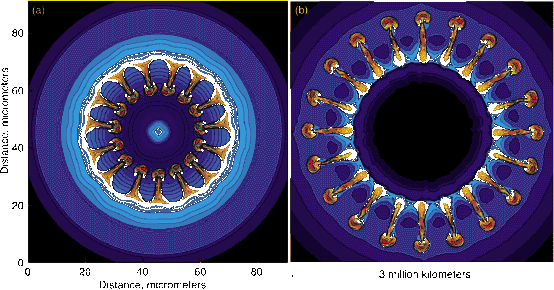
\includegraphics[width=0.55\linewidth]{Figures/ICF.png} %Implosion in ICF, core collapse in supernova
\hspace{1cm} 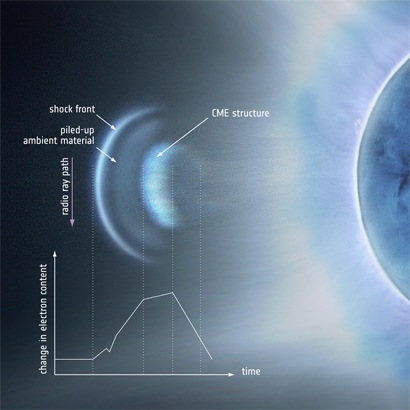
\includegraphics[width=0.32\linewidth]{Figures/cmesketch.jpg} \\ 
\centering 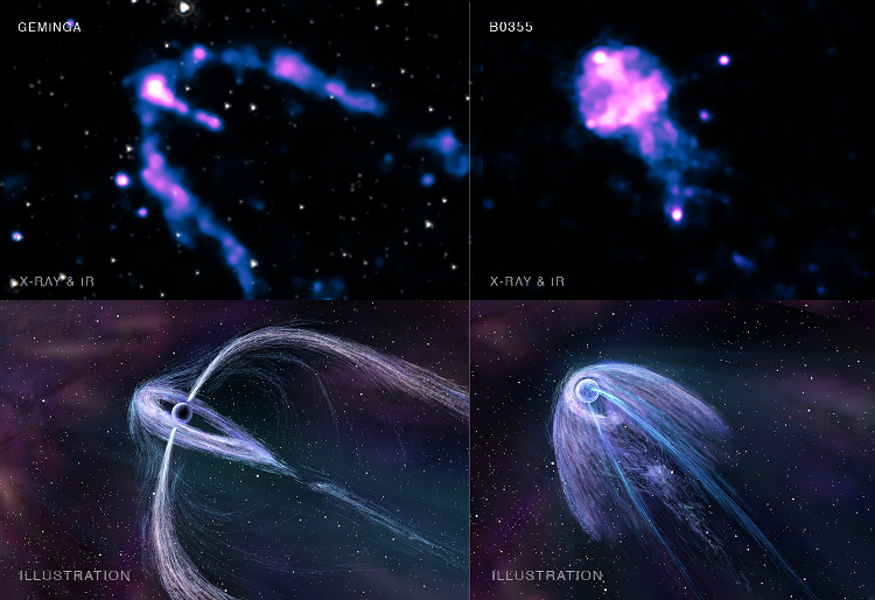
\includegraphics[width=0.32\linewidth]{Figures/pulsarwinds_chandra.jpg} \hspace{2cm}
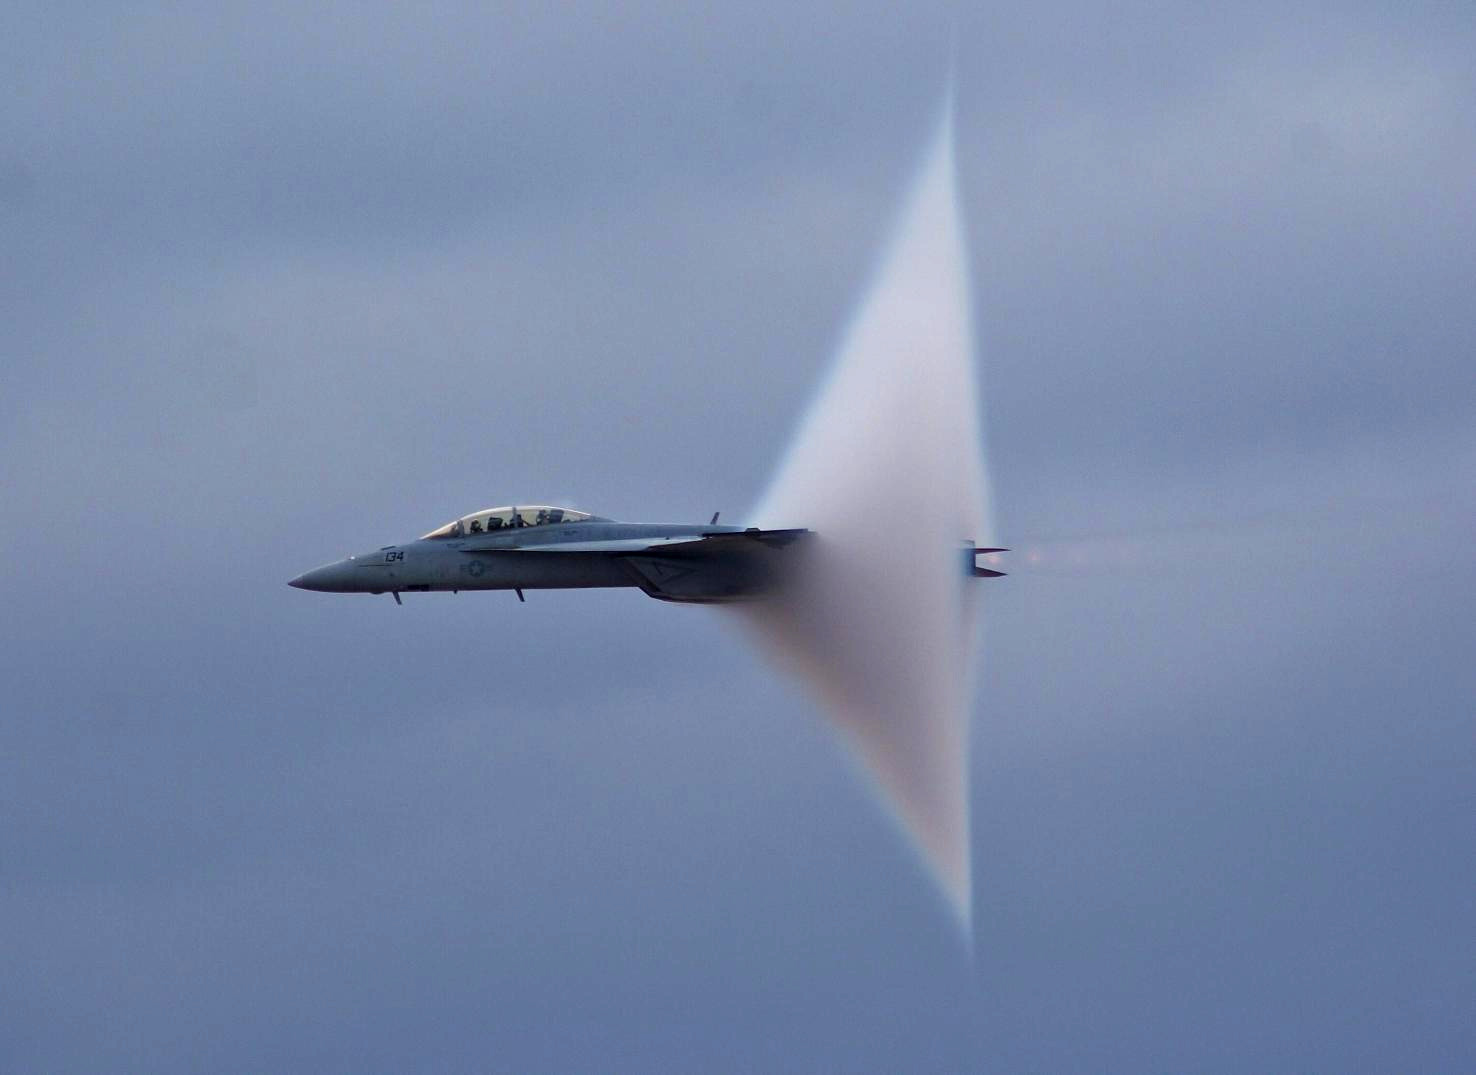
\includegraphics[width=0.32\linewidth]{Figures/FA-18_going_transonic.jpeg}
\end{frame}

% \begin{frame}{Solar Atmosphere - heating mechanisms}
% \begin{itemize}
%     \item AC vs DC
% \end{itemize}
% \end{frame}

% \begin{frame}{Shocks and heating}
% \begin{itemize}
%     \item Intrinsically linked to heating
%     \item Adiabatic (compression) and non-adiabatic (dissipative heating)
% \end{itemize}
% \end{frame}

\begin{frame}{Solar Atmosphere}
\begin{columns}
\begin{column}{0.55\textwidth}
%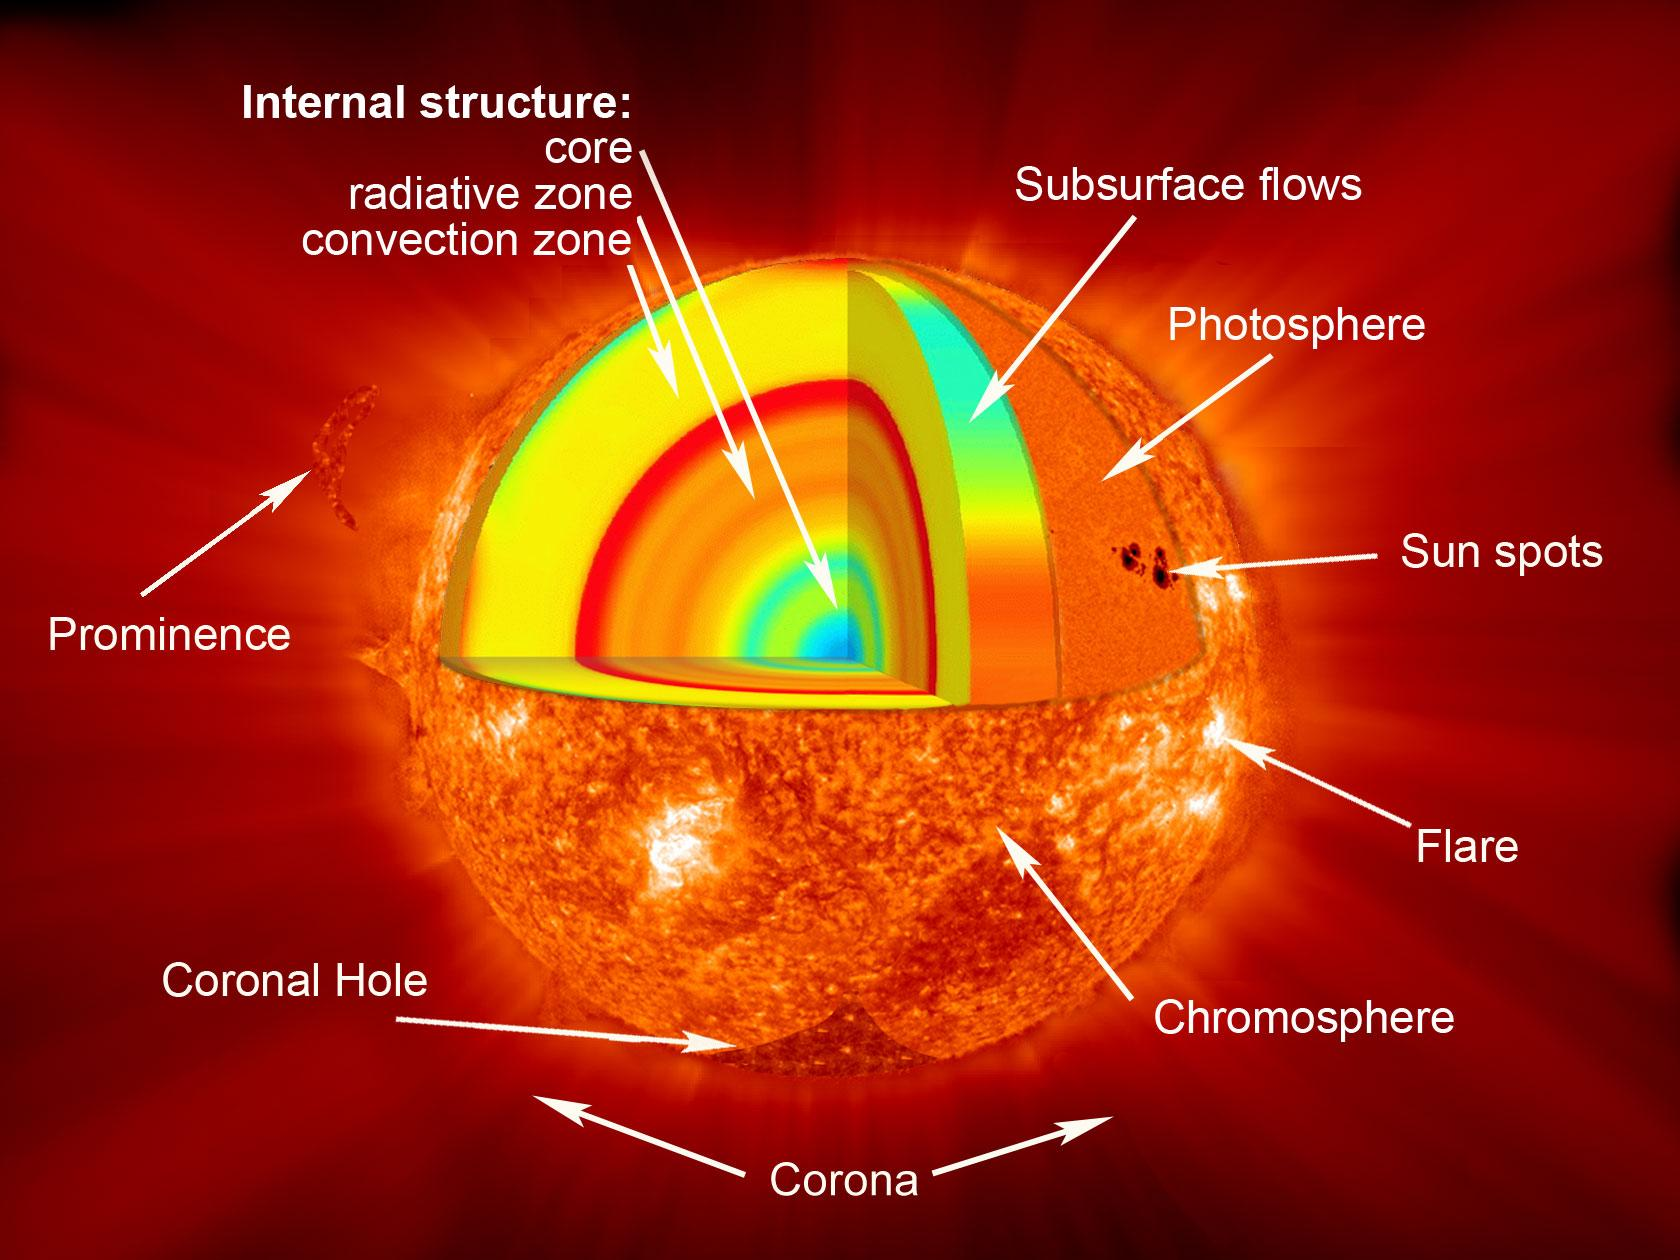
\includegraphics[width=0.9\textwidth]{2023StAndrewsAstro/Figures/462977main_sun_layers_full.jpg}
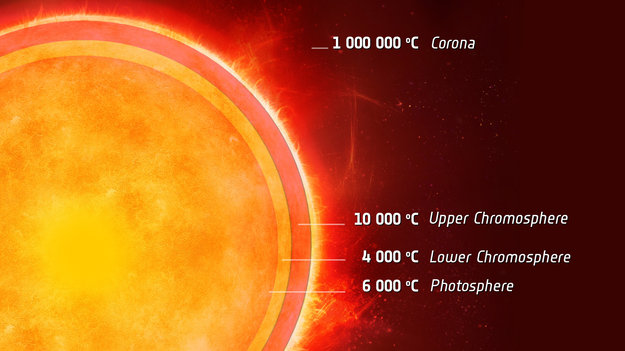
\includegraphics[width=0.9\textwidth]{2023StAndrewsAstro/Figures/sun2.jpg}
\end{column}
\begin{column}{0.45\textwidth}
\begin{itemize}
    \item $R_e \approx 10^4-10^9$ $R_m \approx 10^9-10^{12}$
    \item Chromosphere bridges fluid-dominated surface and magnetic-dominated corona
    \item \textbf{Big problem - heating}. How is the high temperature maintained against the strong radiative losses
    \item Shocks seen as contributor towards heating (adiabatic, non-adiabatic)
\end{itemize}
\end{column}
\end{columns}
\end{frame}

\begin{frame}{Solar Chromosphere}
\begin{columns}
\begin{column}{0.45\textwidth}
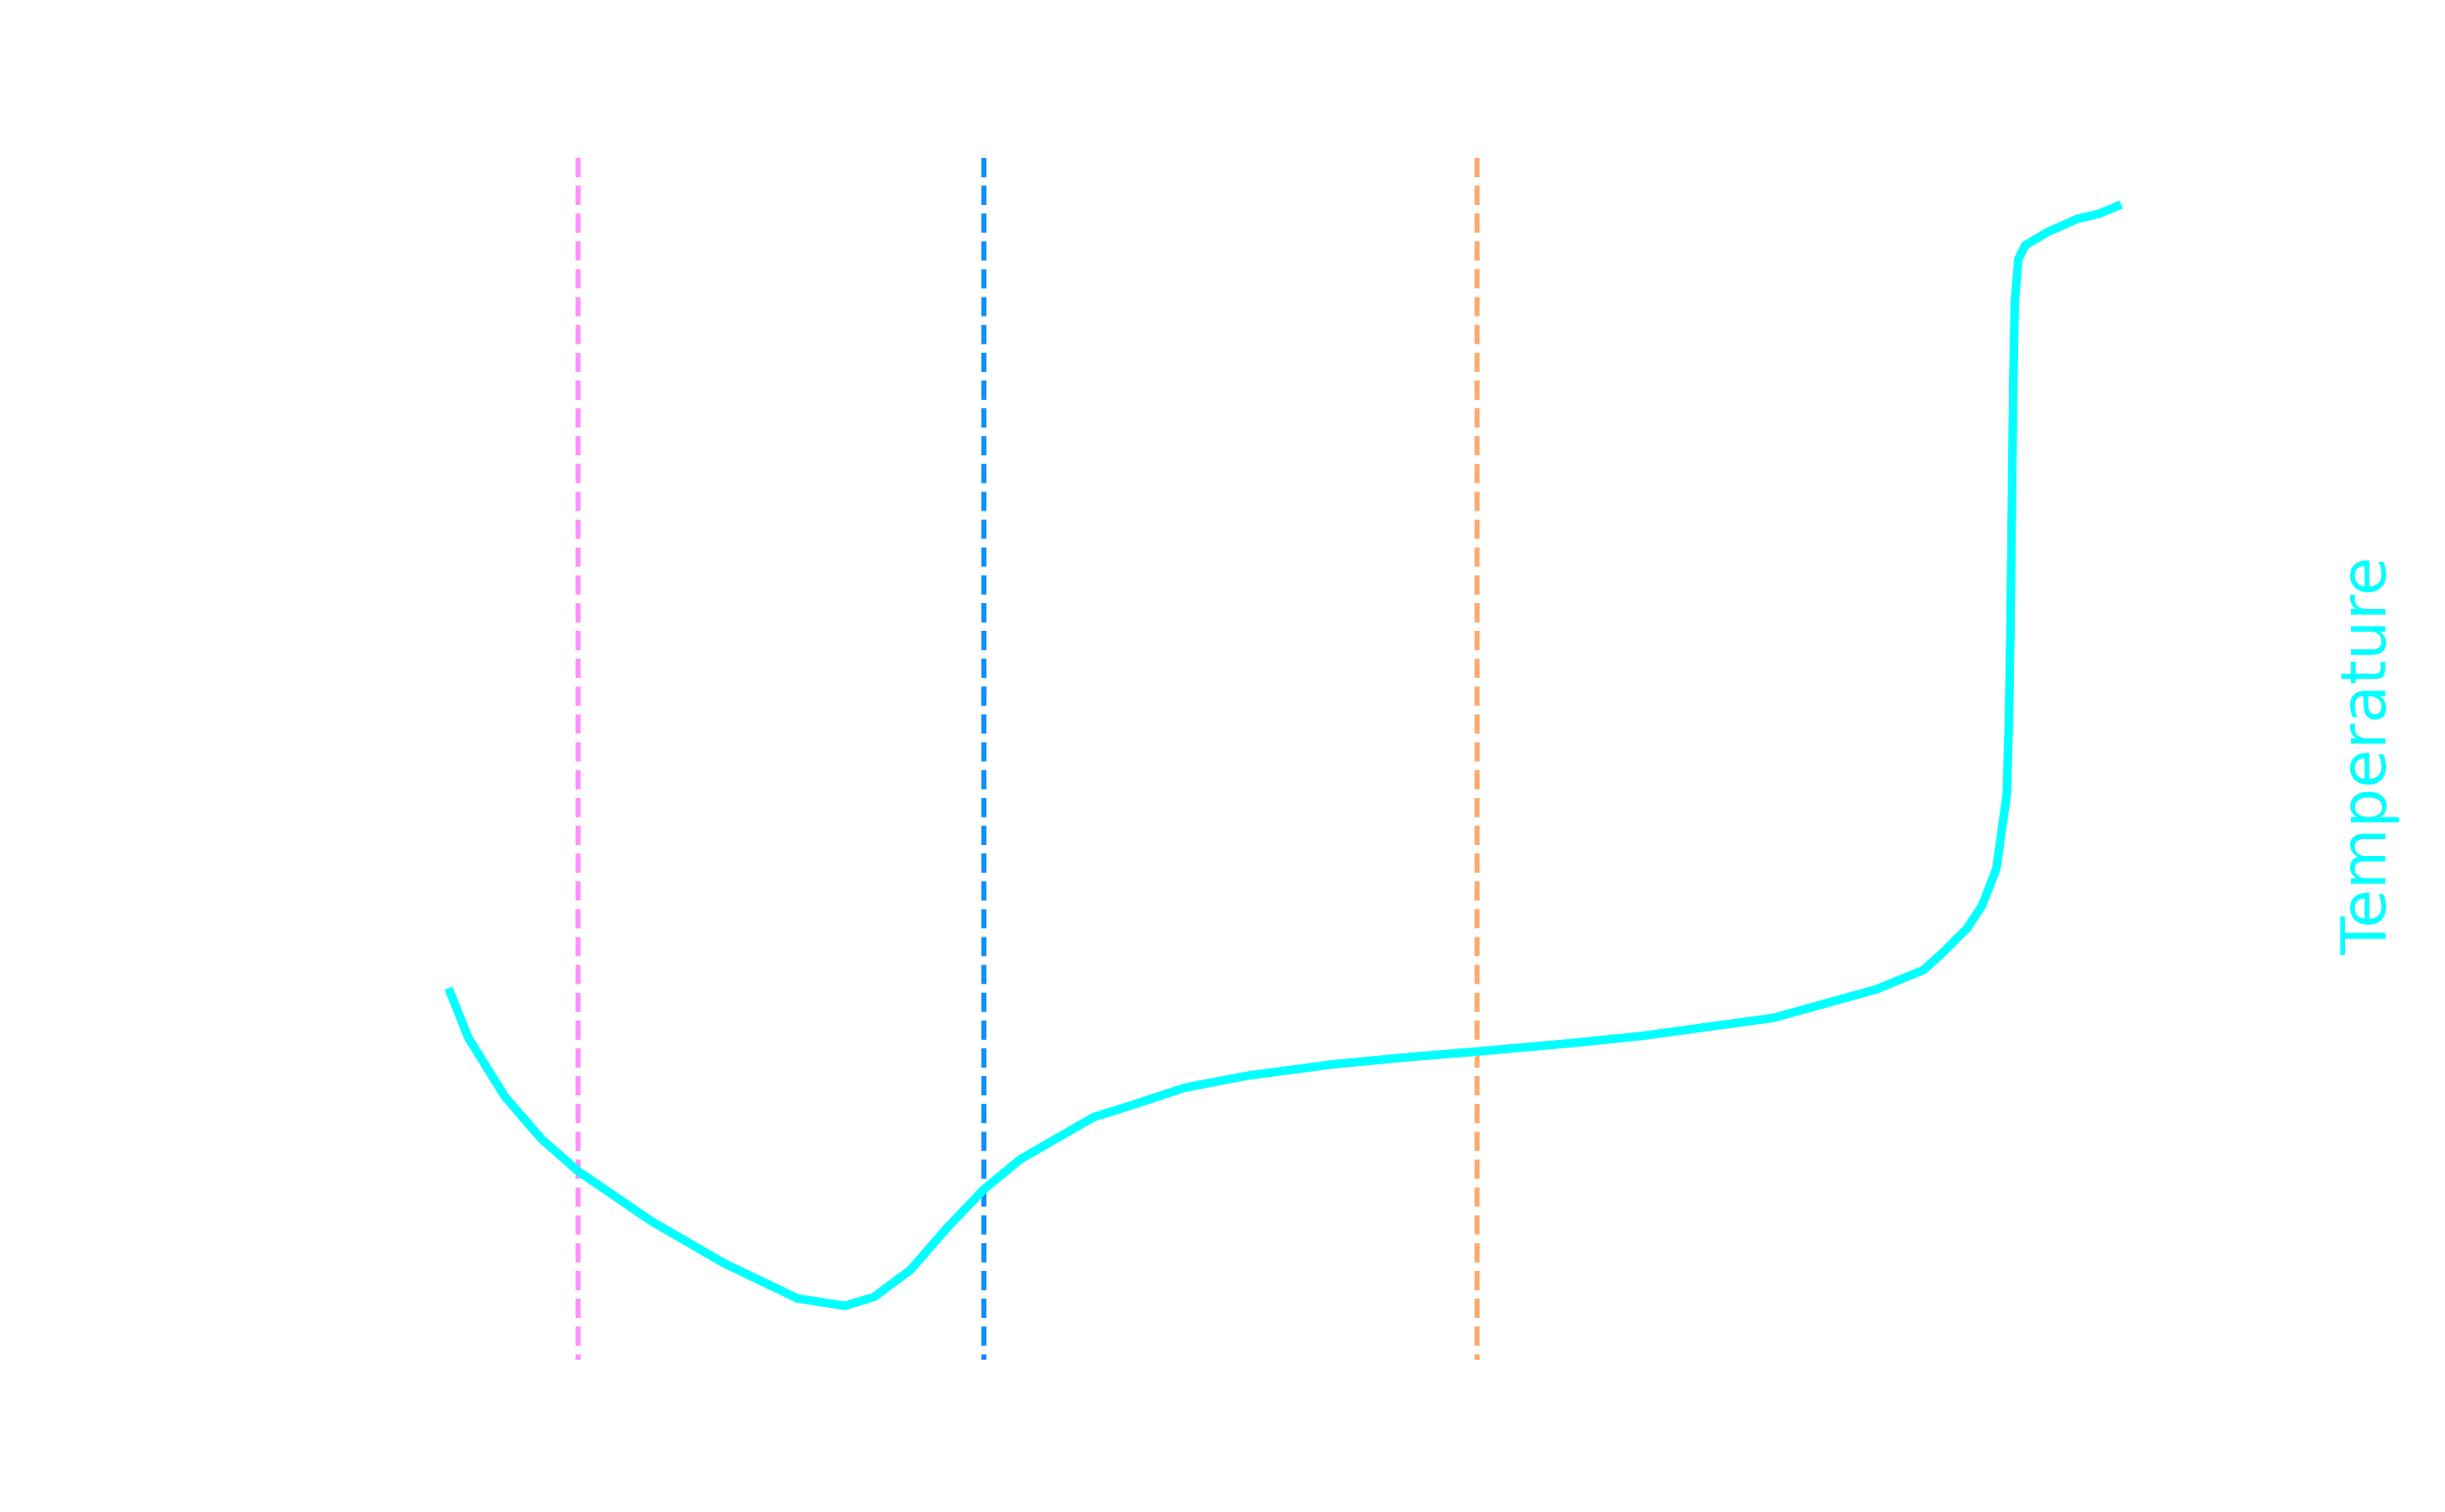
\includegraphics[width=0.95\linewidth]{2023StAndrewsAstro/Figures/saha2_plot.png}
\end{column}
\begin{column}{0.55\textwidth}
\begin{itemize}
    \item Chromosphere is partially ionised - consists of both ionised and neutral species
    \item Interactions between ions and neutral leads to heating, enhanced reconnection rates, changes stability critera....
    \item Shocks regularly observed.
\end{itemize}
\end{column}
\end{columns}
\begin{itemize}
    \item My research aim - role of partially-ionised shocks in heating
    \item Consistent comment from referees - should link to C-, J-shocks in ISM, etc.,
\end{itemize}
\end{frame}

\begin{frame}{Seminar Outline}
\begin{itemize}
    \item Shocks in MHD - ideal solution and limitations
    \item Shocks in partial ionised plasma - the 'standard' model
    \item Comprehensive treatment of partially-ionised plasma
    \item Thermal contribution of partially-ionised shocks
    \item Relating this to astronomical systems
%    \item Substructure possible.
\end{itemize}
\end{frame}

%%%%%%%%%%%%%%%%%%%%%%%%%%%%%%%%%%%%%%%%%%%%%%%%%%%%%%%%%%%%%%%%%%%%%%%%%

\begin{frame}{Ideal MHD Equations}
\footnotesize
\begin{gather}
\frac{\partial \rho}{\partial t} + \nabla \cdot (\rho \textbf{v}) = 0 \\
\frac{\partial}{\partial t} (\rho \textbf{v})+ \nabla \cdot \left( \rho \textbf{v} \textbf{v} + P \textbf{I} - \textbf{B B} + \frac{\textbf{B}^2}{2} \textbf{I} \right) = 0\\
\frac{\partial}{\partial t} \left( e + \frac{\textbf{B}^2}{2} \right) + \nabla \cdot \left[ \textbf{v} ( e + P) -  (\textbf{v} \times \textbf{B}) \times \textbf{B} \right]  =  0 \\
\frac{\partial \textbf{B}}{\partial t} - \nabla \times (\textbf{v} \times \textbf{B}) = 0 \\
\nabla \cdot \textbf{B} =0.
%e_{\text{p}} = \frac{P_{\text{p}}}{\gamma -1} + \frac{1}{2} \rho _{\text{p}} v_{\text{p}} ^2, \\
%\nabla \cdot \textbf{B} = 0,\label{eqn:plasma2}
\end{gather}
\end{frame}

\begin{frame}{Ideal MHD shock jumps}
\begin{columns}
\begin{column}{0.45\textwidth}
\begin{gather}
    \left[\rho v_x  \right]^u _d = 0,  \\
    \left[\rho v_x^2 +P +\frac{B_y^2}{2} \right]^u _d = 0, \\
    \left[\rho v_x v_y -B_x B_y \right]^u _d = 0, \\
    \left[ v_{x} \left( \frac{\gamma}{\gamma -1} P + \frac{1}{2} \rho v^2 \right) \right]^u _d =0, \\
    \left[B_x \right]^u _d = 0, \\
    \left[v_x B_y -v_y B_x   \right]^u _d = 0, 
\end{gather}
% where
% \begin{gather}
%     \left[ Q \right]^u _d \equiv Q^u - Q^d,
% \end{gather}
\end{column}
\begin{column}{0.55\textwidth}
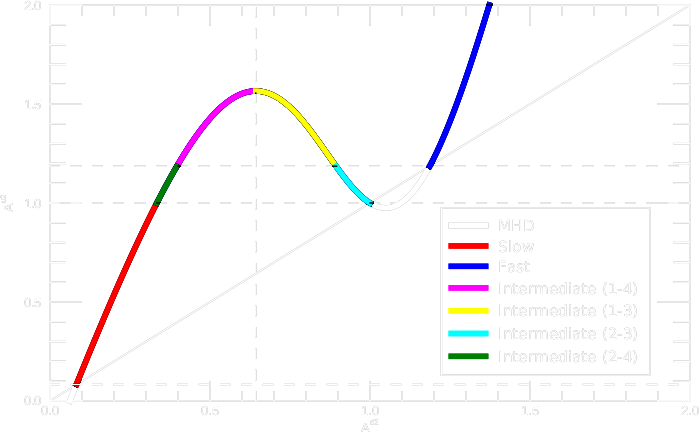
\includegraphics[width=0.95\linewidth]{2023NAM/Figures/shockjumps_0.125pi.png}
\end{column}
\end{columns}
\begin{gather}
    A_\perp ^{\text{u}2} = \frac{ A_\perp ^{\text{d}2} \left( \frac{\gamma-1}{\gamma} \left( \frac{\gamma+1}{\gamma -1} -\tan ^2 \theta \right) \left(A_\perp ^{\text{d}2} -1 \right) ^2 + \tan ^2 \theta  \left( \frac{\gamma-1}{\gamma} A_\perp ^{\text{d}2} -1 \right) \left(A_\perp ^{\text{d}2} -2 \right) \right) - \frac{\beta }{ \cos ^2 \theta } \left( A_\perp ^{\text{d}2} -1 \right) ^2 } { \frac{\gamma -1}{\gamma} \frac{\left( A_\perp ^{\text{d}2}-1 \right) ^2}{ \cos ^2 \theta ^{\text{u}}} - A_ \perp ^{\text{d}2} \tan ^2 \theta ^{\text{u}} \left( \frac{\gamma -1}{\gamma} A_\perp ^{\text{d}2} -1 \right) } \label{eqn:hau}
\end{gather}
\begin{flushright}
{\small Hau+1989}
\end{flushright}
\end{frame}

% \begin{frame}{Partial ionisation}
% \begin{itemize}
%     \item Coupling time-scales in solar atmosphere
% \end{itemize}
% \end{frame}

%%%%%%%%%%%%%%%%%%%%%%%%%%%%%%%%%%%%%%%%%%%%%%%%%%%%%%%%%%%%%%%%%%%%%%%%%
% \begin{frame}{Science Highlight - Shocks in partially ionised plasmas}
% \begin{columns}
% \begin{column}{0.5\textwidth}
% \begin{itemize}
%     \item Big problem - how is the temperature of the solar atmosphere maintained against the strong losses?
%     \item Shocks are regularly observed in the solar atmosphere and are seen as a contributor to heating.
%     \item Adiabatic (compression) \& non-adiabatic (dissipative)
%     \item But is this really whats going on?
%     %\item But it is not this simple, most magnetic energy is in the potential field component, so how do we get free magnetic energy into the corona?
% \end{itemize}
% \end{column}
% \begin{column}{0.5\textwidth}
% %\includegraphics[width=0.32\linewidth]{Figures/Crab_Nebula.jpeg}
% 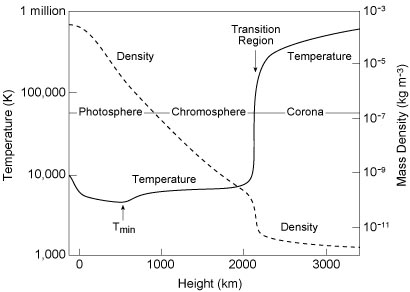
\includegraphics[width=0.95\linewidth]{2023Dundee/Figures/valc.png}
% %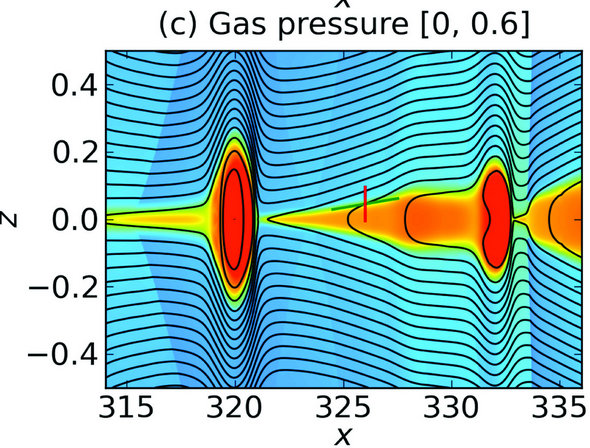
\includegraphics[width=0.95\linewidth]{2023RAS/Figures/shibyama.png}
% %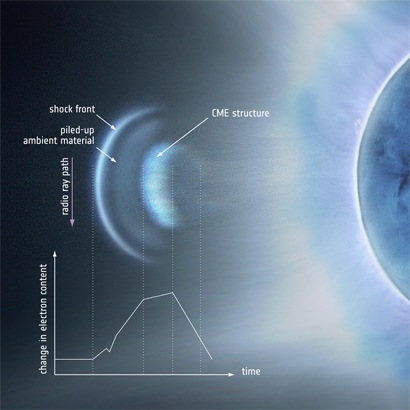
\includegraphics[width=0.32\linewidth]{Figures/cmesketch.jpg}
% \end{column}
% \end{columns}
% \end{frame}

% \begin{frame}{MHD (conservative)}
% \begin{columns}
% \begin{column}{0.4\textwidth}
% \begin{itemize}
%     \item Stable shock solutions can be analytically determined by the upstream plasma-$\beta$, angle of magnetic field $\theta$, and Alfven Mach numbers.
%     \item Shocks heat!
%     \item True for any conservative set of MHD equations
%     \item But are these the correct set of equations to use for the solar atmosphere?
% \end{itemize}
% \end{column}
% \begin{column}{0.6\textwidth}
% %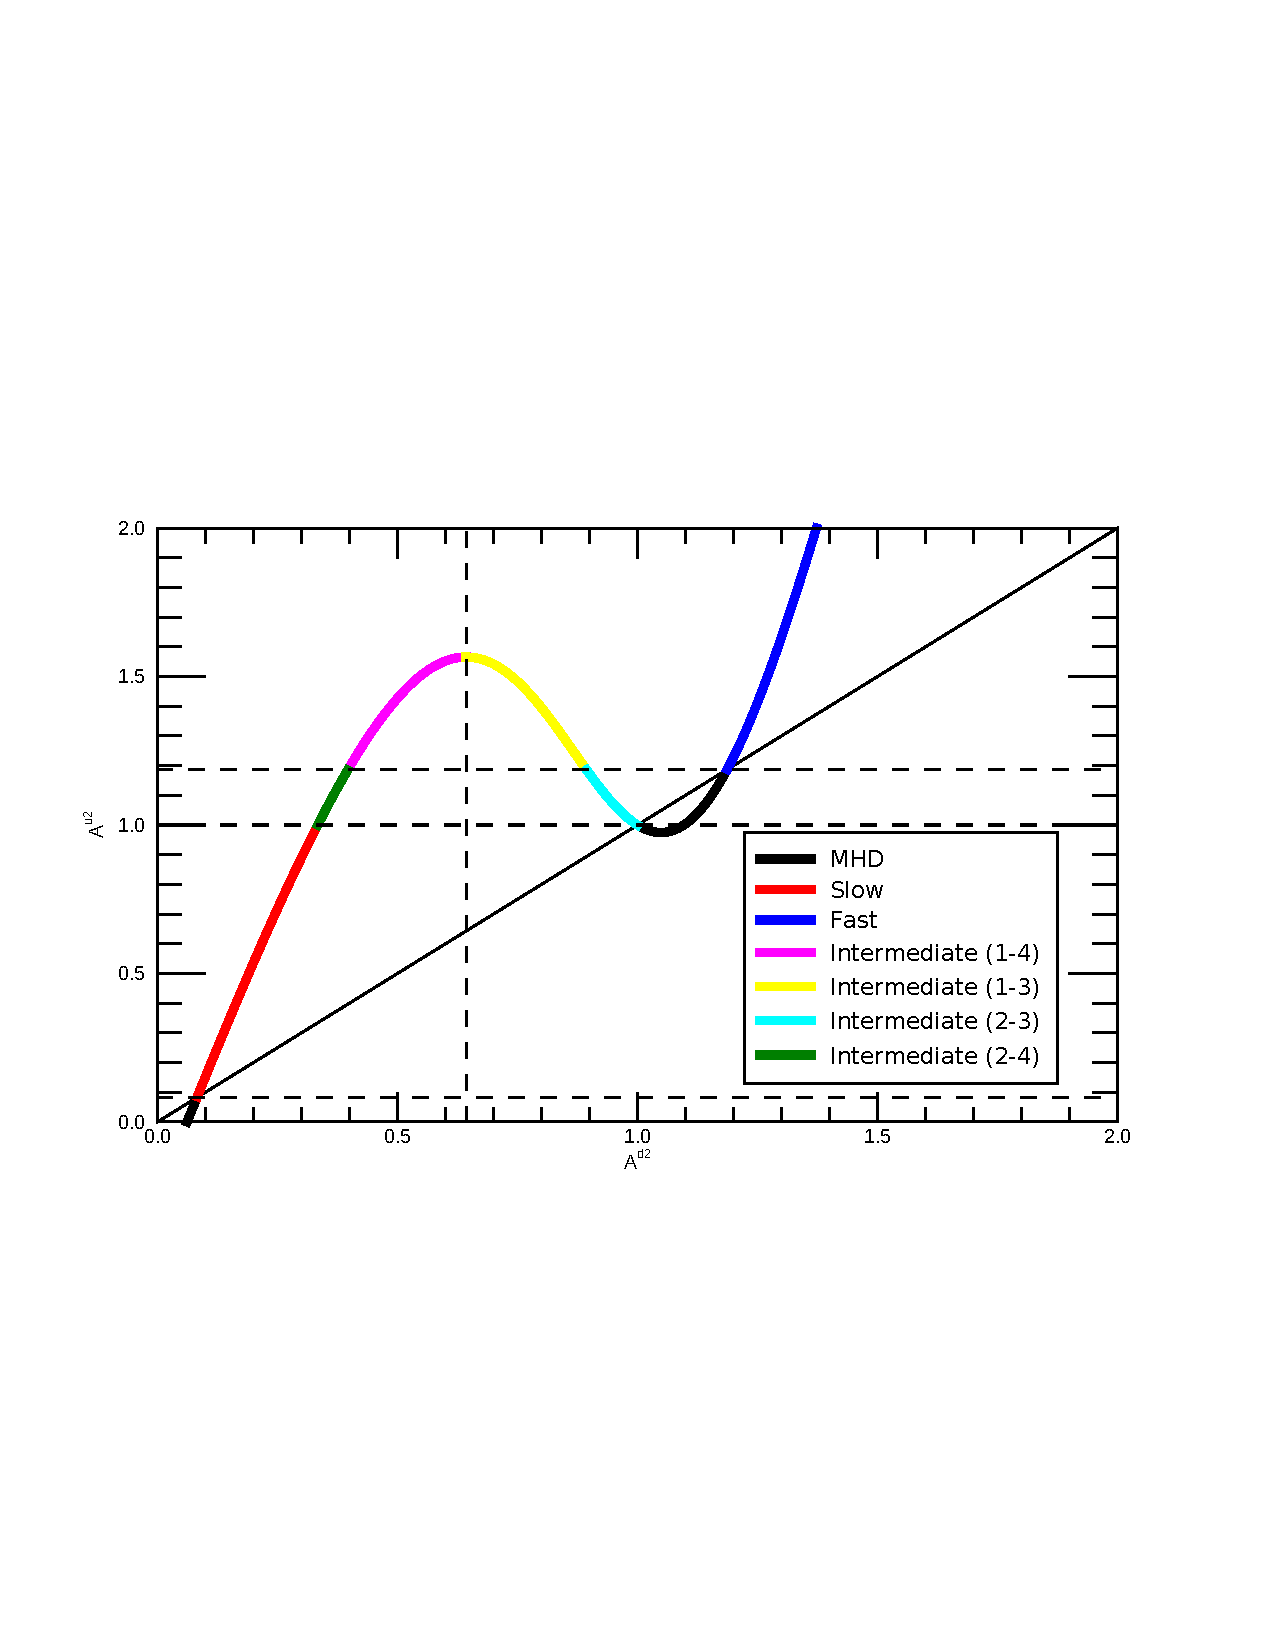
\includegraphics[width=0.95\linewidth,clip=true,trim=1.0cm 8.0cm 2.5cm 8.5cm]{2023NAM/Figures/shockjumps_0.125pi.pdf}
% 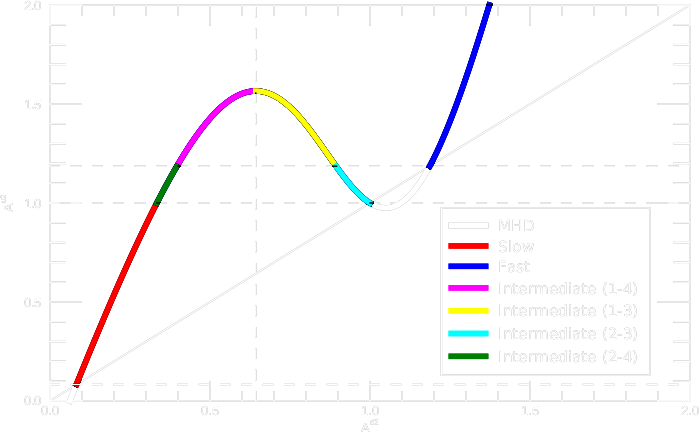
\includegraphics[width=0.95\linewidth]{2023NAM/Figures/shockjumps_0.125pi.png}
% \end{column}
% \end{columns}
% \begin{gather}
%     A_\perp ^{\text{u}2} = \frac{ A_\perp ^{\text{d}2} \left( \frac{\gamma-1}{\gamma} \left( \frac{\gamma+1}{\gamma -1} -\tan ^2 \theta \right) \left(A_\perp ^{\text{d}2} -1 \right) ^2 + \tan ^2 \theta  \left( \frac{\gamma-1}{\gamma} A_\perp ^{\text{d}2} -1 \right) \left(A_\perp ^{\text{d}2} -2 \right) \right) - \frac{\beta }{ \cos ^2 \theta } \left( A_\perp ^{\text{d}2} -1 \right) ^2 } { \frac{\gamma -1}{\gamma} \frac{\left( A_\perp ^{\text{d}2}-1 \right) ^2}{ \cos ^2 \theta ^{\text{u}}} - A_ \perp ^{\text{d}2} \tan ^2 \theta ^{\text{u}} \left( \frac{\gamma -1}{\gamma} A_\perp ^{\text{d}2} -1 \right) } \label{eqn:hau}
% \end{gather}
% \begin{flushright}
% {\small Hau+1989}
% \end{flushright}
% \end{frame}

\begin{frame}{Partially ionised chromosphere}
\begin{columns}
\begin{column}{0.5\textwidth}
\begin{itemize}
    \item Chromosphere is partially ionised - ions and neutrals follow different equations.
    \item Partial ionisation known to speed up magnetic reconnection, dissipative heating of Alfven waves, affect stability of systems (KHI, RT, corrugation)
    \item Two-fluid shocks not well understood - high frequency events lead to localised decoupling of ions and neutrals
    % \item Missing physics: ionisation/recombination rates increased in shocks, multiple excited neutral hydrogen states, non-equilibrium ionisation, ionisation/excitation cooling, recombination/de-excitation heating..... 
\end{itemize}
\end{column}
\begin{column}{0.5\textwidth}
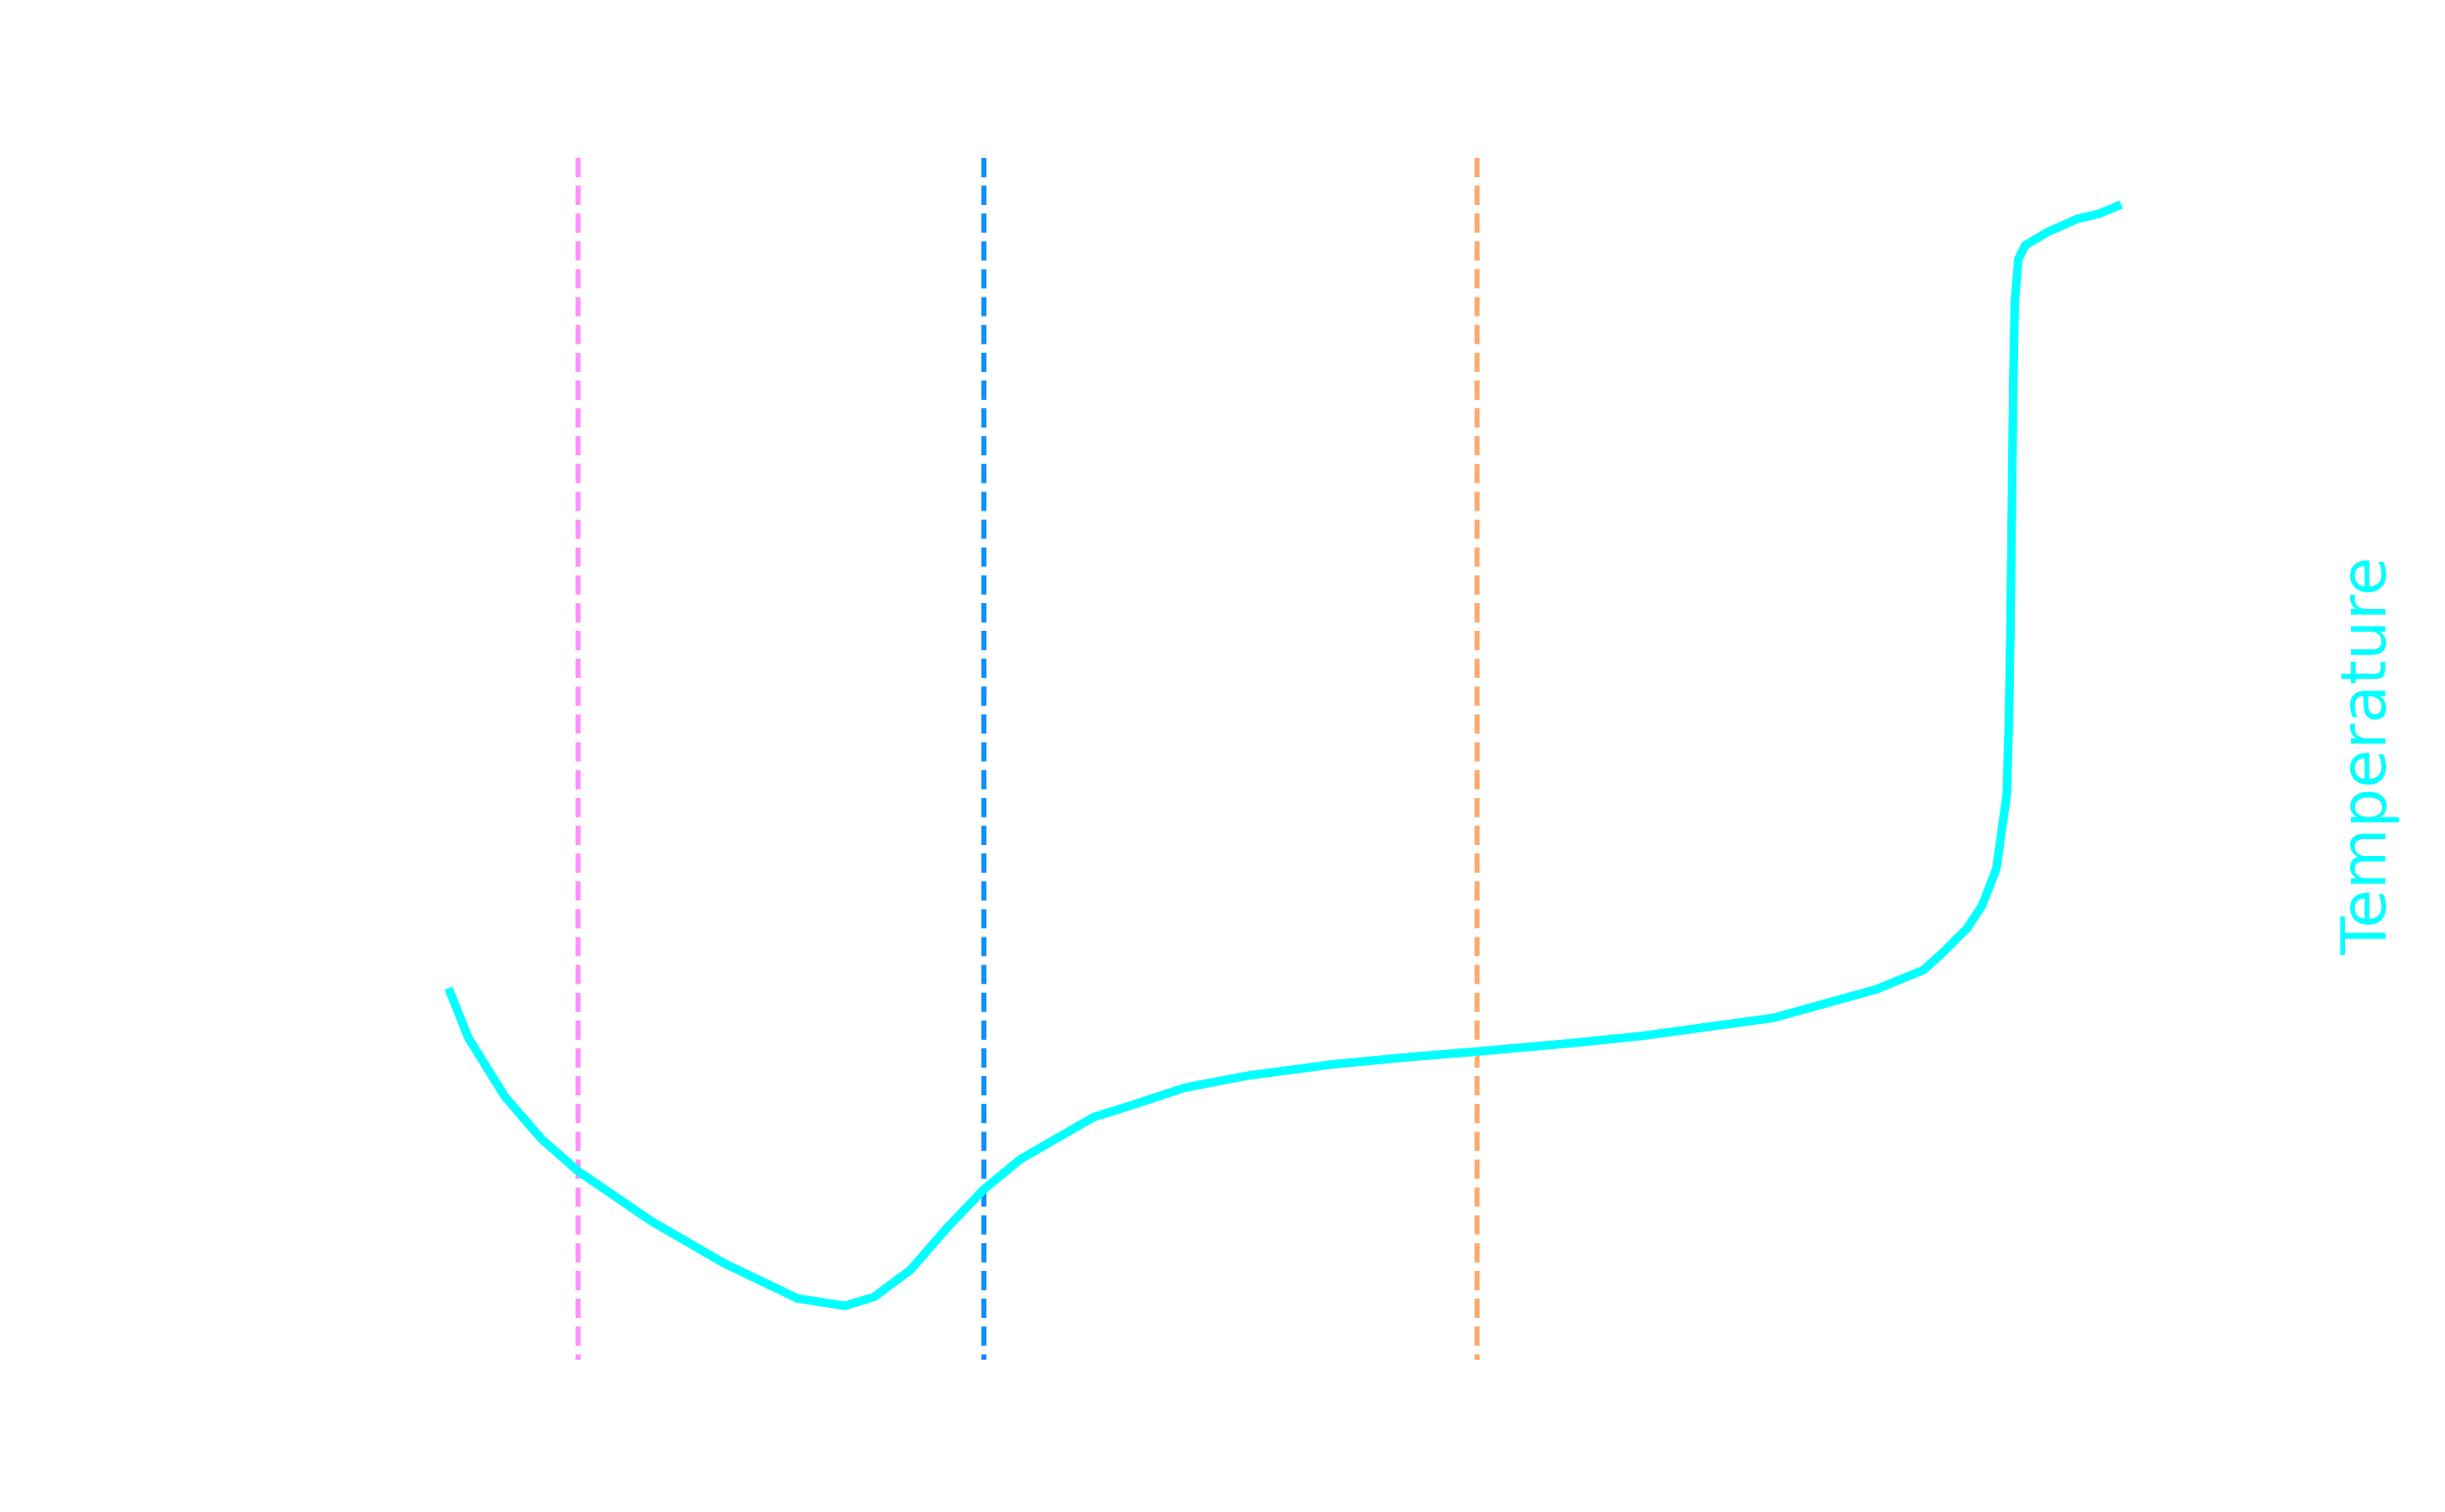
\includegraphics[width=0.9\linewidth]{2023StAndrewsAstro/Figures/saha2_plot.png} \\
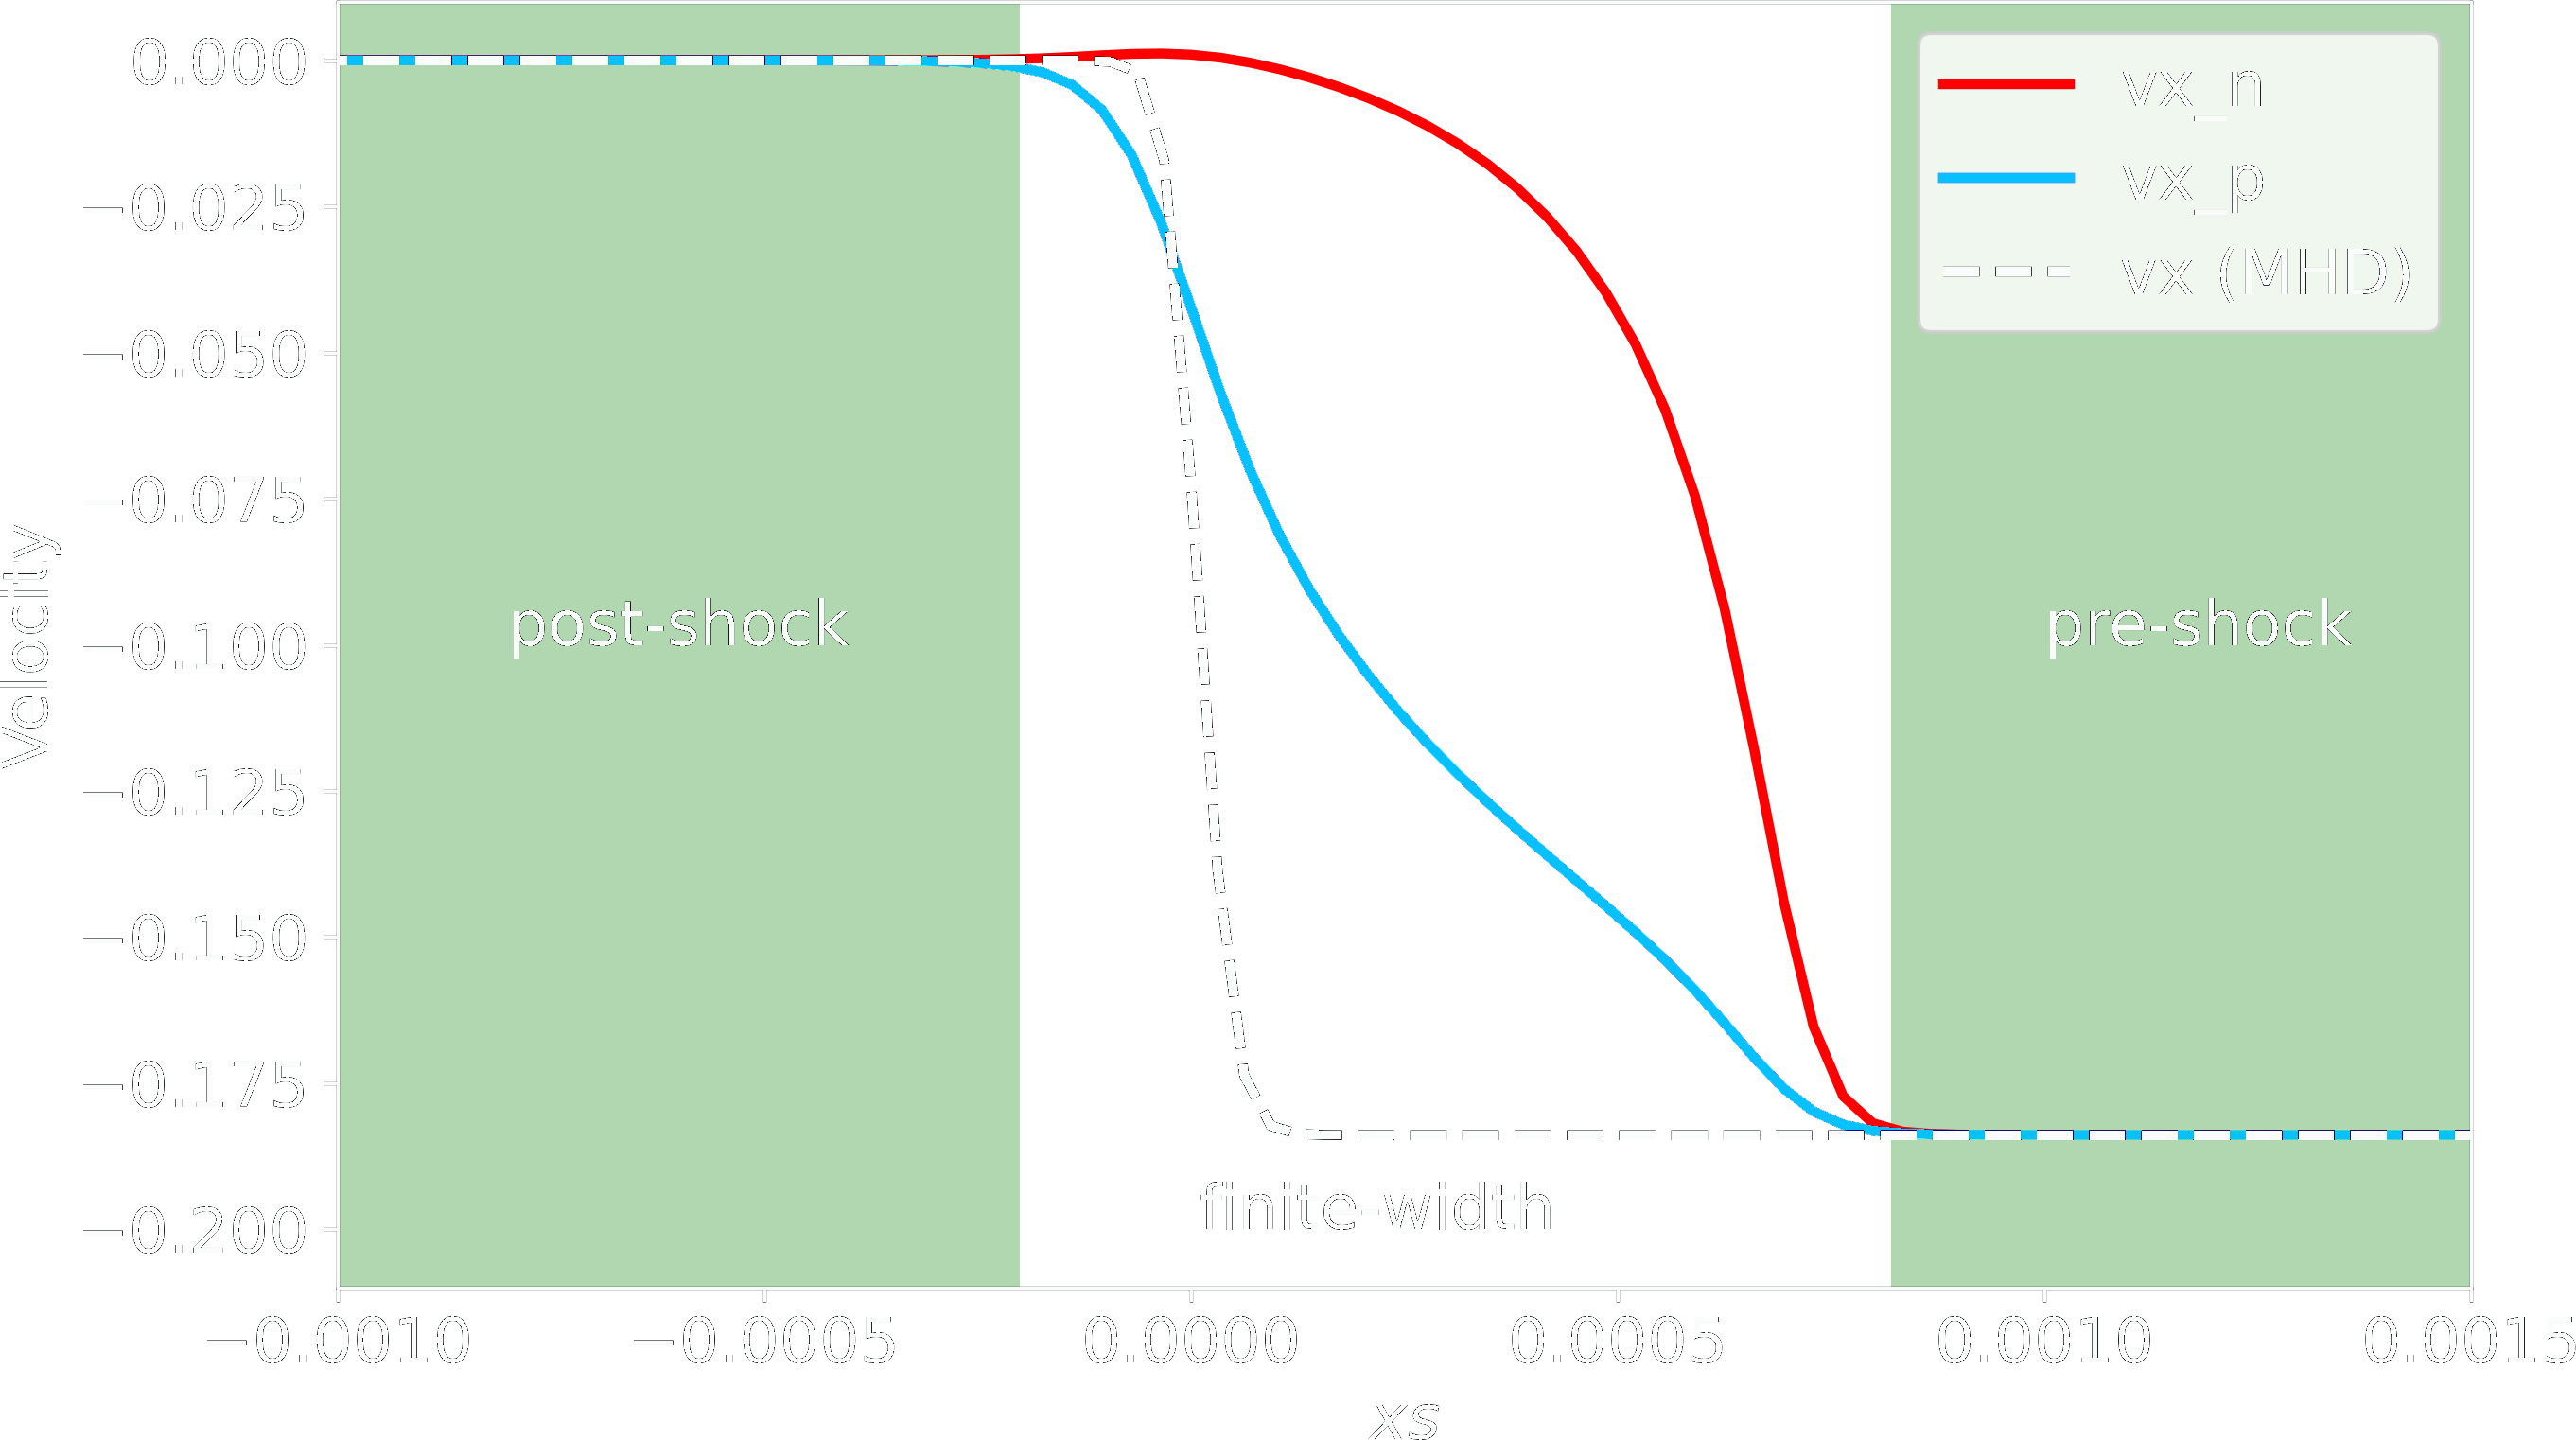
\includegraphics[width=0.95\linewidth]{2023StAndrewsAstro/Figures/shocksub_col.png} \\
%Conservative equations (e.g., two-fluid with thermal collisions) leads to MHD shock jumps, Snow \& Hillier 2019.
\end{column}
\end{columns}
\end{frame}

\begin{frame}{Ionisation, recombination and ionisation potential in two-fluid shocks}
\footnotesize
\begin{gather}
\frac{\partial \rho _{\text{n}}}{\partial t} + \nabla \cdot (\rho _{\text{n}} \textbf{v}_{\text{n}})= \Gamma _{rec} \rho _{\rm p} - \Gamma _{ion} \rho _{\rm n}, \label{eqn:neutral1}\tag{5} \\
\frac{\partial}{\partial t}(\rho _{\text{n}} \textbf{v}_{\text{n}}) + \nabla \cdot (\rho _{\text{n}} \textbf{v}_{\text{n}} \textbf{v}_{\text{n}} + P_{\text{n}} \textbf{I}) = -\alpha _c \rho_{\text{n}} \rho_{\text{p}} (\textbf{v}_{\text{n}}-\textbf{v}_{\text{p}}) + \Gamma _{rec} \rho _{\rm p} \textbf{v}_{\rm p} - \Gamma _{ion} \rho_{\rm n} \textbf{v}_{\rm n}, \tag{6}\\
\frac{\partial e_{\text{n}}}{\partial t} + \nabla \cdot \left[\textbf{v}_{\text{n}} (e_{\text{n}} +P_{\text{n}}) \right] = -\alpha _c \rho _{\text{n}} \rho _{\text{p}} \left[ \frac{1}{2} (\textbf{v}_{\text{n}} ^2 - \textbf{v}_{\text{p}} ^2)+ \frac{3}{2} \left(\frac{P_{\rm n}}{\rho_{\rm n}}-\frac{1}{2}\frac{P_{\rm p}}{\rho_{\rm p}}\right) \right] \nonumber \\ \hspace{0.5cm}+ \frac{1}{2} \left( \Gamma _{rec} \rho _{\rm p} \textbf{v}_{\rm p} ^2 - \Gamma _{ion} \rho _{\rm n} \textbf{v}_{\rm n} ^2 \right) +\frac{1}{ (\gamma-1)} \left( \frac{1}{2} \Gamma _{rec} P_{\rm p} -\Gamma _{ion} P_{\rm n} \right), \tag{7}\\
%e_{\text{n}} = \frac{P_{\text{n}}}{\gamma -1} + \frac{1}{2} \rho _{\text{n}} v_{\text{n}} ^2, \label{eqn:neutral2} \\
\frac{\partial \rho _{\text{p}}}{\partial t} + \nabla \cdot (\rho_{\text{p}} \textbf{v}_{\text{p}}) = - \Gamma _{rec} \rho _{\rm p} + \Gamma _{ion} \rho _{\rm n} \label{eqn:plasma1}\tag{8}\\
\frac{\partial}{\partial t} (\rho_{\text{p}} \textbf{v}_{\text{p}})+ \nabla \cdot \left( \rho_{\text{p}} \textbf{v}_{\text{p}} \textbf{v}_{\text{p}} + P_{\text{p}} \textbf{I} - \textbf{B B} + \frac{\textbf{B}^2}{2} \textbf{I} \right) = \alpha _c \rho_{\text{n}} \rho_{\text{p}}(\textbf{v}_{\text{n}} - \textbf{v}_{\text{p}}) - \Gamma _{rec} \rho _{\rm p} \textbf{v}_{\rm p} + \Gamma _{ion} \rho_{\rm n} \textbf{v}_{\rm n},\tag{9}\\
\frac{\partial}{\partial t} \left( e_{\text{p}} + \frac{\textbf{B}^2}{2} \right) + \nabla \cdot \left[ \textbf{v}_{\text{p}} ( e_{\text{p}} + P_{\text{p}}) -  (\textbf{v}_{\rm p} \times \textbf{B}) \times \textbf{B} \right]  =  \alpha _c \rho _{\text{n}} \rho _{\text{p}} \left[ \frac{1}{2} (\textbf{v}_{\text{n}} ^2 - \textbf{v}_{\text{p}} ^2)+ \frac{3}{2} \left(\frac{P_{\rm n}}{\rho_{\rm n}}-\frac{1}{2}\frac{P_{\rm p}}{\rho_{\rm p}}\right) \right] \nonumber \\ \hspace{0.5cm}- \frac{1}{2} \left( \Gamma _{rec} \rho _{\rm p} \textbf{v}_{\rm p} ^2 - \Gamma _{ion} \rho _{\rm n} \textbf{v}_{\rm n} ^2 \right) {- \phi_I + \phi_{heat}} -\frac{1}{ (\gamma-1)} \left( \frac{1}{2} \Gamma _{rec} P_{\rm p} -\Gamma _{ion} P_{\rm n} \right), \label{eqn:ep}\tag{10} \\
\frac{\partial \textbf{B}}{\partial t} - \nabla \times (\textbf{v}_{\text{p}} \times \textbf{B}) = 0.\tag{11}
%e_{\text{p}} = \frac{P_{\text{p}}}{\gamma -1} + \frac{1}{2} \rho _{\text{p}} v_{\text{p}} ^2, \\
%\nabla \cdot \textbf{B} = 0,\label{eqn:plasma2}
\end{gather}
\end{frame}

\begin{frame}{Ionisation, recombination and ionisation potential in two-fluid shocks}
\vspace{-0.5cm}
\footnotesize
\begin{gather}
\mathcolorbox{VioletRed}{\frac{\partial \rho _{\text{n}}}{\partial t} + \nabla \cdot (\rho _{\text{n}} \textbf{v}_{\text{n}})}= \Gamma _{rec} \rho _{\rm p} - \Gamma _{ion} \rho _{\rm n}, \label{eqn:neutral1}\tag{5} \\
\mathcolorbox{VioletRed}{\frac{\partial}{\partial t}(\rho _{\text{n}} \textbf{v}_{\text{n}}) + \nabla \cdot (\rho _{\text{n}} \textbf{v}_{\text{n}} \textbf{v}_{\text{n}} + P_{\text{n}} \textbf{I})} = -\alpha _c \rho_{\text{n}} \rho_{\text{p}} (\textbf{v}_{\text{n}}-\textbf{v}_{\text{p}}) + \Gamma _{rec} \rho _{\rm p} \textbf{v}_{\rm p} - \Gamma _{ion} \rho_{\rm n} \textbf{v}_{\rm n}, \tag{6}\\
\mathcolorbox{VioletRed}{\frac{\partial e_{\text{n}}}{\partial t} + \nabla \cdot \left[\textbf{v}_{\text{n}} (e_{\text{n}} +P_{\text{n}}) \right]} = -\alpha _c \rho _{\text{n}} \rho _{\text{p}} \left[ \frac{1}{2} (\textbf{v}_{\text{n}} ^2 - \textbf{v}_{\text{p}} ^2)+ \frac{3}{2} \left(\frac{P_{\rm n}}{\rho_{\rm n}}-\frac{1}{2}\frac{P_{\rm p}}{\rho_{\rm p}}\right) \right] \nonumber \\ \hspace{0.5cm}+ \frac{1}{2} \left( \Gamma _{rec} \rho _{\rm p} \textbf{v}_{\rm p} ^2 - \Gamma _{ion} \rho _{\rm n} \textbf{v}_{\rm n} ^2 \right) +\frac{1}{ (\gamma-1)} \left( \frac{1}{2} \Gamma _{rec} P_{\rm p} -\Gamma _{ion} P_{\rm n} \right), \tag{7}\\
%e_{\text{n}} = \frac{P_{\text{n}}}{\gamma -1} + \frac{1}{2} \rho _{\text{n}} v_{\text{n}} ^2, \label{eqn:neutral2} \\
\frac{\partial \rho _{\text{p}}}{\partial t} + \nabla \cdot (\rho_{\text{p}} \textbf{v}_{\text{p}}) = - \Gamma _{rec} \rho _{\rm p} + \Gamma _{ion} \rho _{\rm n} \label{eqn:plasma1}\tag{8}\\
\frac{\partial}{\partial t} (\rho_{\text{p}} \textbf{v}_{\text{p}})+ \nabla \cdot \left( \rho_{\text{p}} \textbf{v}_{\text{p}} \textbf{v}_{\text{p}} + P_{\text{p}} \textbf{I} - \textbf{B B} + \frac{\textbf{B}^2}{2} \textbf{I} \right) = \alpha _c \rho_{\text{n}} \rho_{\text{p}}(\textbf{v}_{\text{n}} - \textbf{v}_{\text{p}}) - \Gamma _{rec} \rho _{\rm p} \textbf{v}_{\rm p} + \Gamma _{ion} \rho_{\rm n} \textbf{v}_{\rm n},\tag{9}\\
\frac{\partial}{\partial t} \left( e_{\text{p}} + \frac{\textbf{B}^2}{2} \right) + \nabla \cdot \left[ \textbf{v}_{\text{p}} ( e_{\text{p}} + P_{\text{p}}) -  (\textbf{v}_{\rm p} \times \textbf{B}) \times \textbf{B} \right]  =  \alpha _c \rho _{\text{n}} \rho _{\text{p}} \left[ \frac{1}{2} (\textbf{v}_{\text{n}} ^2 - \textbf{v}_{\text{p}} ^2)+ \frac{3}{2} \left(\frac{P_{\rm n}}{\rho_{\rm n}}-\frac{1}{2}\frac{P_{\rm p}}{\rho_{\rm p}}\right) \right] \nonumber \\ \hspace{0.5cm}- \frac{1}{2} \left( \Gamma _{rec} \rho _{\rm p} \textbf{v}_{\rm p} ^2 - \Gamma _{ion} \rho _{\rm n} \textbf{v}_{\rm n} ^2 \right) {- \phi_I + \phi_{heat}} -\frac{1}{ (\gamma-1)} \left( \frac{1}{2} \Gamma _{rec} P_{\rm p} -\Gamma _{ion} P_{\rm n} \right), \label{eqn:ep} \tag{10}\\
\frac{\partial \textbf{B}}{\partial t} - \nabla \times (\textbf{v}_{\text{p}} \times \textbf{B}) = 0.\tag{11}
%e_{\text{p}} = \frac{P_{\text{p}}}{\gamma -1} + \frac{1}{2} \rho _{\text{p}} v_{\text{p}} ^2, \\
%\nabla \cdot \textbf{B} = 0,\label{eqn:plasma2}
\end{gather}
\end{frame}

\begin{frame}{Ionisation, recombination and ionisation potential in two-fluid shocks}
\vspace{-0.5cm}
\footnotesize
\begin{gather}
\frac{\partial \rho _{\text{n}}}{\partial t} + \nabla \cdot (\rho _{\text{n}} \textbf{v}_{\text{n}})= \Gamma _{rec} \rho _{\rm p} - \Gamma _{ion} \rho _{\rm n}, \label{eqn:neutral1}\tag{5} \\
\frac{\partial}{\partial t}(\rho _{\text{n}} \textbf{v}_{\text{n}}) + \nabla \cdot (\rho _{\text{n}} \textbf{v}_{\text{n}} \textbf{v}_{\text{n}} + P_{\text{n}} \textbf{I}) = -\alpha _c \rho_{\text{n}} \rho_{\text{p}} (\textbf{v}_{\text{n}}-\textbf{v}_{\text{p}}) + \Gamma _{rec} \rho _{\rm p} \textbf{v}_{\rm p} - \Gamma _{ion} \rho_{\rm n} \textbf{v}_{\rm n}, \tag{6}\\
\frac{\partial e_{\text{n}}}{\partial t} + \nabla \cdot \left[\textbf{v}_{\text{n}} (e_{\text{n}} +P_{\text{n}}) \right] = -\alpha _c \rho _{\text{n}} \rho _{\text{p}} \left[ \frac{1}{2} (\textbf{v}_{\text{n}} ^2 - \textbf{v}_{\text{p}} ^2)+ \frac{3}{2} \left(\frac{P_{\rm n}}{\rho_{\rm n}}-\frac{1}{2}\frac{P_{\rm p}}{\rho_{\rm p}}\right) \right] \nonumber \\ \hspace{0.5cm}+ \frac{1}{2} \left( \Gamma _{rec} \rho _{\rm p} \textbf{v}_{\rm p} ^2 - \Gamma _{ion} \rho _{\rm n} \textbf{v}_{\rm n} ^2 \right) +\frac{1}{ (\gamma-1)} \left( \frac{1}{2} \Gamma _{rec} P_{\rm p} -\Gamma _{ion} P_{\rm n} \right), \tag{7}\\
%e_{\text{n}} = \frac{P_{\text{n}}}{\gamma -1} + \frac{1}{2} \rho _{\text{n}} v_{\text{n}} ^2, \label{eqn:neutral2} \\
\mathcolorbox{BlueGreen}{\frac{\partial \rho _{\text{p}}}{\partial t} + \nabla \cdot (\rho_{\text{p}} \textbf{v}_{\text{p}})} = - \Gamma _{rec} \rho _{\rm p} + \Gamma _{ion} \rho _{\rm n} \label{eqn:plasma1}\tag{8}\\
\mathcolorbox{BlueGreen}{\frac{\partial}{\partial t} (\rho_{\text{p}} \textbf{v}_{\text{p}})+ \nabla \cdot \left( \rho_{\text{p}} \textbf{v}_{\text{p}} \textbf{v}_{\text{p}} + P_{\text{p}} \textbf{I} - \textbf{B B} + \frac{\textbf{B}^2}{2} \textbf{I} \right)} = \alpha _c \rho_{\text{n}} \rho_{\text{p}}(\textbf{v}_{\text{n}} - \textbf{v}_{\text{p}}) - \Gamma _{rec} \rho _{\rm p} \textbf{v}_{\rm p} + \Gamma _{ion} \rho_{\rm n} \textbf{v}_{\rm n},\tag{9}\\
\mathcolorbox{BlueGreen}{\frac{\partial}{\partial t} \left( e_{\text{p}} + \frac{\textbf{B}^2}{2} \right) + \nabla \cdot \left[ \textbf{v}_{\text{p}} ( e_{\text{p}} + P_{\text{p}}) -  (\textbf{v}_{\rm p} \times \textbf{B}) \times \textbf{B} \right] } =  \alpha _c \rho _{\text{n}} \rho _{\text{p}} \left[ \frac{1}{2} (\textbf{v}_{\text{n}} ^2 - \textbf{v}_{\text{p}} ^2)+ \frac{3}{2} \left(\frac{P_{\rm n}}{\rho_{\rm n}}-\frac{1}{2}\frac{P_{\rm p}}{\rho_{\rm p}}\right) \right] \nonumber \\ \hspace{0.5cm}- \frac{1}{2} \left( \Gamma _{rec} \rho _{\rm p} \textbf{v}_{\rm p} ^2 - \Gamma _{ion} \rho _{\rm n} \textbf{v}_{\rm n} ^2 \right) {- \phi_I + \phi_{heat}} -\frac{1}{ (\gamma-1)} \left( \frac{1}{2} \Gamma _{rec} P_{\rm p} -\Gamma _{ion} P_{\rm n} \right), \label{eqn:ep}\tag{10} \\
\mathcolorbox{BlueGreen}{\frac{\partial \textbf{B}}{\partial t} - \nabla \times (\textbf{v}_{\text{p}} \times \textbf{B}) = 0.}\tag{11}
%e_{\text{p}} = \frac{P_{\text{p}}}{\gamma -1} + \frac{1}{2} \rho _{\text{p}} v_{\text{p}} ^2, \\
%\nabla \cdot \textbf{B} = 0,\label{eqn:plasma2}
\end{gather}
\end{frame}

\begin{frame}{Ionisation, recombination and ionisation potential in two-fluid shocks}
\vspace{-0.5cm}
\footnotesize
\begin{gather}
\frac{\partial \rho _{\text{n}}}{\partial t} + \nabla \cdot (\rho _{\text{n}} \textbf{v}_{\text{n}})= \Gamma _{rec} \rho _{\rm p} - \Gamma _{ion} \rho _{\rm n}, \label{eqn:neutral1}\tag{5} \\
\frac{\partial}{\partial t}(\rho _{\text{n}} \textbf{v}_{\text{n}}) + \nabla \cdot (\rho _{\text{n}} \textbf{v}_{\text{n}} \textbf{v}_{\text{n}} + P_{\text{n}} \textbf{I}) =\mathcolorbox{YellowOrange}{ -\alpha _c \rho_{\text{n}} \rho_{\text{p}} (\textbf{v}_{\text{n}}-\textbf{v}_{\text{p}})} + \Gamma _{rec} \rho _{\rm p} \textbf{v}_{\rm p} - \Gamma _{ion} \rho_{\rm n} \textbf{v}_{\rm n}, \tag{6}\\
\frac{\partial e_{\text{n}}}{\partial t} + \nabla \cdot \left[\textbf{v}_{\text{n}} (e_{\text{n}} +P_{\text{n}}) \right] = \mathcolorbox{YellowOrange}{-\alpha _c \rho _{\text{n}} \rho _{\text{p}} \left[ \frac{1}{2} (\textbf{v}_{\text{n}} ^2 - \textbf{v}_{\text{p}} ^2)+ \frac{3}{2} \left(\frac{P_{\rm n}}{\rho_{\rm n}}-\frac{1}{2}\frac{P_{\rm p}}{\rho_{\rm p}}\right) \right]} \nonumber \\ \hspace{0.5cm}+ \frac{1}{2} \left( \Gamma _{rec} \rho _{\rm p} \textbf{v}_{\rm p} ^2 - \Gamma _{ion} \rho _{\rm n} \textbf{v}_{\rm n} ^2 \right) +\frac{1}{ (\gamma-1)} \left( \frac{1}{2} \Gamma _{rec} P_{\rm p} -\Gamma _{ion} P_{\rm n} \right), \tag{7}\\
%e_{\text{n}} = \frac{P_{\text{n}}}{\gamma -1} + \frac{1}{2} \rho _{\text{n}} v_{\text{n}} ^2, \label{eqn:neutral2} \\
\frac{\partial \rho _{\text{p}}}{\partial t} + \nabla \cdot (\rho_{\text{p}} \textbf{v}_{\text{p}}) = - \Gamma _{rec} \rho _{\rm p} + \Gamma _{ion} \rho _{\rm n} \label{eqn:plasma1}\tag{8}\\
\frac{\partial}{\partial t} (\rho_{\text{p}} \textbf{v}_{\text{p}})+ \nabla \cdot \left( \rho_{\text{p}} \textbf{v}_{\text{p}} \textbf{v}_{\text{p}} + P_{\text{p}} \textbf{I} - \textbf{B B} + \frac{\textbf{B}^2}{2} \textbf{I} \right) = \mathcolorbox{YellowOrange}{\alpha _c \rho_{\text{n}} \rho_{\text{p}}(\textbf{v}_{\text{n}} - \textbf{v}_{\text{p}})} - \Gamma _{rec} \rho _{\rm p} \textbf{v}_{\rm p} + \Gamma _{ion} \rho_{\rm n} \textbf{v}_{\rm n},\tag{9}\\
\frac{\partial}{\partial t} \left( e_{\text{p}} + \frac{\textbf{B}^2}{2} \right) + \nabla \cdot \left[ \textbf{v}_{\text{p}} ( e_{\text{p}} + P_{\text{p}}) -  (\textbf{v}_{\rm p} \times \textbf{B}) \times \textbf{B} \right]  = \mathcolorbox{YellowOrange}{ \alpha _c \rho _{\text{n}} \rho _{\text{p}} \left[ \frac{1}{2} (\textbf{v}_{\text{n}} ^2 - \textbf{v}_{\text{p}} ^2)+ \frac{3}{2} \left(\frac{P_{\rm n}}{\rho_{\rm n}}-\frac{1}{2}\frac{P_{\rm p}}{\rho_{\rm p}}\right) \right]} \nonumber \\ \hspace{0.5cm}- \frac{1}{2} \left( \Gamma _{rec} \rho _{\rm p} \textbf{v}_{\rm p} ^2 - \Gamma _{ion} \rho _{\rm n} \textbf{v}_{\rm n} ^2 \right) {- \phi_I + \phi_{heat}} -\frac{1}{ (\gamma-1)} \left( \frac{1}{2} \Gamma _{rec} P_{\rm p} -\Gamma _{ion} P_{\rm n} \right), \label{eqn:ep} \tag{10}\\
\frac{\partial \textbf{B}}{\partial t} - \nabla \times (\textbf{v}_{\text{p}} \times \textbf{B}) = 0.\tag{11}
%e_{\text{p}} = \frac{P_{\text{p}}}{\gamma -1} + \frac{1}{2} \rho _{\text{p}} v_{\text{p}} ^2, \\
%\nabla \cdot \textbf{B} = 0,\label{eqn:plasma2}
\end{gather}
\end{frame}

\begin{frame}{Ionisation, recombination and ionisation potential in two-fluid shocks}
\vspace{-0.5cm}
\footnotesize
\begin{gather}
\frac{\partial \rho _{\text{n}}}{\partial t} + \nabla \cdot (\rho _{\text{n}} \textbf{v}_{\text{n}})= \mathcolorbox{LimeGreen}{\Gamma _{rec} \rho _{\rm p} - \Gamma _{ion} \rho _{\rm n},} \label{eqn:neutral1}\tag{5} \\
\frac{\partial}{\partial t}(\rho _{\text{n}} \textbf{v}_{\text{n}}) + \nabla \cdot (\rho _{\text{n}} \textbf{v}_{\text{n}} \textbf{v}_{\text{n}} + P_{\text{n}} \textbf{I}) = -\alpha _c \rho_{\text{n}} \rho_{\text{p}} (\textbf{v}_{\text{n}}-\textbf{v}_{\text{p}}) + \mathcolorbox{LimeGreen}{\Gamma _{rec} \rho _{\rm p} \textbf{v}_{\rm p} - \Gamma _{ion} \rho_{\rm n} \textbf{v}_{\rm n}}, \tag{6}\\
\frac{\partial e_{\text{n}}}{\partial t} + \nabla \cdot \left[\textbf{v}_{\text{n}} (e_{\text{n}} +P_{\text{n}}) \right] = -\alpha _c \rho _{\text{n}} \rho _{\text{p}} \left[ \frac{1}{2} (\textbf{v}_{\text{n}} ^2 - \textbf{v}_{\text{p}} ^2)+ \frac{3}{2} \left(\frac{P_{\rm n}}{\rho_{\rm n}}-\frac{1}{2}\frac{P_{\rm p}}{\rho_{\rm p}}\right) \right] \nonumber \\ \hspace{0.5cm}+ \mathcolorbox{LimeGreen}{\frac{1}{2} \left( \Gamma _{rec} \rho _{\rm p} \textbf{v}_{\rm p} ^2 - \Gamma _{ion} \rho _{\rm n} \textbf{v}_{\rm n} ^2 \right) +\frac{1}{ (\gamma-1)} \left( \frac{1}{2} \Gamma _{rec} P_{\rm p} -\Gamma _{ion} P_{\rm n} \right),} \tag{7}\\
%e_{\text{n}} = \frac{P_{\text{n}}}{\gamma -1} + \frac{1}{2} \rho _{\text{n}} v_{\text{n}} ^2, \label{eqn:neutral2} \\
\frac{\partial \rho _{\text{p}}}{\partial t} + \nabla \cdot (\rho_{\text{p}} \textbf{v}_{\text{p}}) = \mathcolorbox{LimeGreen}{- \Gamma _{rec} \rho _{\rm p} + \Gamma _{ion} \rho _{\rm n}} \label{eqn:plasma1}\tag{8}\\
\frac{\partial}{\partial t} (\rho_{\text{p}} \textbf{v}_{\text{p}})+ \nabla \cdot \left( \rho_{\text{p}} \textbf{v}_{\text{p}} \textbf{v}_{\text{p}} + P_{\text{p}} \textbf{I} - \textbf{B B} + \frac{\textbf{B}^2}{2} \textbf{I} \right) = \alpha _c \rho_{\text{n}} \rho_{\text{p}}(\textbf{v}_{\text{n}} - \textbf{v}_{\text{p}}) \mathcolorbox{LimeGreen}{- \Gamma _{rec} \rho _{\rm p} \textbf{v}_{\rm p} + \Gamma _{ion} \rho_{\rm n} \textbf{v}_{\rm n},}\tag{9}\\
\frac{\partial}{\partial t} \left( e_{\text{p}} + \frac{\textbf{B}^2}{2} \right) + \nabla \cdot \left[ \textbf{v}_{\text{p}} ( e_{\text{p}} + P_{\text{p}}) -  (\textbf{v}_{\rm p} \times \textbf{B}) \times \textbf{B} \right]  =  \alpha _c \rho _{\text{n}} \rho _{\text{p}} \left[ \frac{1}{2} (\textbf{v}_{\text{n}} ^2 - \textbf{v}_{\text{p}} ^2)+ \frac{3}{2} \left(\frac{P_{\rm n}}{\rho_{\rm n}}-\frac{1}{2}\frac{P_{\rm p}}{\rho_{\rm p}}\right) \right] \nonumber \\ \hspace{0.5cm}\mathcolorbox{LimeGreen}{- \frac{1}{2} \left( \Gamma _{rec} \rho _{\rm p} \textbf{v}_{\rm p} ^2 - \Gamma _{ion} \rho _{\rm n} \textbf{v}_{\rm n} ^2 \right)} {- \phi_I + \phi_{heat}} \mathcolorbox{LimeGreen}{-\frac{1}{ (\gamma-1)} \left( \frac{1}{2} \Gamma _{rec} P_{\rm p} -\Gamma _{ion} P_{\rm n} \right)}, \label{eqn:ep} \tag{10}\\
\frac{\partial \textbf{B}}{\partial t} - \nabla \times (\textbf{v}_{\text{p}} \times \textbf{B}) = 0.\tag{11}
%e_{\text{p}} = \frac{P_{\text{p}}}{\gamma -1} + \frac{1}{2} \rho _{\text{p}} v_{\text{p}} ^2, \\
%\nabla \cdot \textbf{B} = 0,\label{eqn:plasma2}
\end{gather}
\end{frame}

\begin{frame}{Ionisation process}
\begin{columns}
\begin{column}{0.4\textwidth}
\begin{itemize}
    % \item Solar chromosphere is partially ionised.
    % \item Understanding two-fluid shocks is fundamental to understanding energy transfer and heating in the solar chromosphere and corona.
    \item Ionisation is a three-body process
    \item Free electron deposits energy to release bound electron
    \item Net loss of energy from the plasma during ionisation
%    \item Substructure possible.
\end{itemize}
%\includegraphics[width=1.0\textwidth,clip=true,trim=1.0cm 1.0cm 1.0cm 1.0cm]{obs_shockloc_contour.png}
\end{column}
\begin{column}{0.6\textwidth}
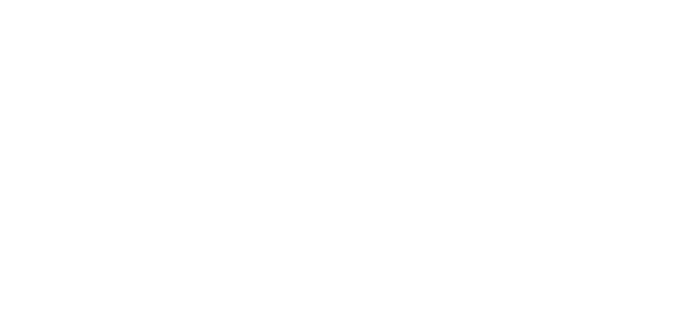
\includegraphics[width=0.95\linewidth]{2023DundeeInterview/Figures/hydrogensketchion_inv.png} 
\end{column}
\end{columns}
\end{frame}

\begin{frame}{Ionisation, recombination and ionisation potential in two-fluid shocks}
\footnotesize
\begin{gather}
\frac{\partial \rho _{\text{n}}}{\partial t} + \nabla \cdot (\rho _{\text{n}} \textbf{v}_{\text{n}})= \Gamma _{rec} \rho _{\rm p} - \Gamma _{ion} \rho _{\rm n}, \label{eqn:neutral1}\tag{5} \\
\frac{\partial}{\partial t}(\rho _{\text{n}} \textbf{v}_{\text{n}}) + \nabla \cdot (\rho _{\text{n}} \textbf{v}_{\text{n}} \textbf{v}_{\text{n}} + P_{\text{n}} \textbf{I}) = -\alpha _c \rho_{\text{n}} \rho_{\text{p}} (\textbf{v}_{\text{n}}-\textbf{v}_{\text{p}}) + \Gamma _{rec} \rho _{\rm p} \textbf{v}_{\rm p} - \Gamma _{ion} \rho_{\rm n} \textbf{v}_{\rm n},\tag{6} \\
\frac{\partial e_{\text{n}}}{\partial t} + \nabla \cdot \left[\textbf{v}_{\text{n}} (e_{\text{n}} +P_{\text{n}}) \right] = -\alpha _c \rho _{\text{n}} \rho _{\text{p}} \left[ \frac{1}{2} (\textbf{v}_{\text{n}} ^2 - \textbf{v}_{\text{p}} ^2)+ \frac{3}{2} \left(\frac{P_{\rm n}}{\rho_{\rm n}}-\frac{1}{2}\frac{P_{\rm p}}{\rho_{\rm p}}\right) \right] \nonumber \\ \hspace{0.5cm}+ \frac{1}{2} \left( \Gamma _{rec} \rho _{\rm p} \textbf{v}_{\rm p} ^2 - \Gamma _{ion} \rho _{\rm n} \textbf{v}_{\rm n} ^2 \right) +\frac{1}{ (\gamma-1)} \left( \frac{1}{2} \Gamma _{rec} P_{\rm p} -\Gamma _{ion} P_{\rm n} \right), \tag{7}\\
%e_{\text{n}} = \frac{P_{\text{n}}}{\gamma -1} + \frac{1}{2} \rho _{\text{n}} v_{\text{n}} ^2, \label{eqn:neutral2} \\
\frac{\partial \rho _{\text{p}}}{\partial t} + \nabla \cdot (\rho_{\text{p}} \textbf{v}_{\text{p}}) = - \Gamma _{rec} \rho _{\rm p} + \Gamma _{ion} \rho _{\rm n} \label{eqn:plasma1}\tag{8}\\
\frac{\partial}{\partial t} (\rho_{\text{p}} \textbf{v}_{\text{p}})+ \nabla \cdot \left( \rho_{\text{p}} \textbf{v}_{\text{p}} \textbf{v}_{\text{p}} + P_{\text{p}} \textbf{I} - \textbf{B B} + \frac{\textbf{B}^2}{2} \textbf{I} \right) = \alpha _c \rho_{\text{n}} \rho_{\text{p}}(\textbf{v}_{\text{n}} - \textbf{v}_{\text{p}}) - \Gamma _{rec} \rho _{\rm p} \textbf{v}_{\rm p} + \Gamma _{ion} \rho_{\rm n} \textbf{v}_{\rm n},\tag{9}\\
\frac{\partial}{\partial t} \left( e_{\text{p}} + \frac{\textbf{B}^2}{2} \right) + \nabla \cdot \left[ \textbf{v}_{\text{p}} ( e_{\text{p}} + P_{\text{p}}) -  (\textbf{v}_{\rm p} \times \textbf{B}) \times \textbf{B} \right]  =  \alpha _c \rho _{\text{n}} \rho _{\text{p}} \left[ \frac{1}{2} (\textbf{v}_{\text{n}} ^2 - \textbf{v}_{\text{p}} ^2)+ \frac{3}{2} \left(\frac{P_{\rm n}}{\rho_{\rm n}}-\frac{1}{2}\frac{P_{\rm p}}{\rho_{\rm p}}\right) \right] \nonumber \\ \hspace{0.5cm}- \frac{1}{2} \left( \Gamma _{rec} \rho _{\rm p} \textbf{v}_{\rm p} ^2 - \Gamma _{ion} \rho _{\rm n} \textbf{v}_{\rm n} ^2 \right) \mathcolorbox{pink}{- \phi_I + \phi_{heat}} -\frac{1}{ (\gamma-1)} \left( \frac{1}{2} \Gamma _{rec} P_{\rm p} -\Gamma _{ion} P_{\rm n} \right), \label{eqn:ep} \tag{10}\\
\frac{\partial \textbf{B}}{\partial t} - \nabla \times (\textbf{v}_{\text{p}} \times \textbf{B}) = 0.\tag{11}
%e_{\text{p}} = \frac{P_{\text{p}}}{\gamma -1} + \frac{1}{2} \rho _{\text{p}} v_{\text{p}} ^2, \\
%\nabla \cdot \textbf{B} = 0,\label{eqn:plasma2}
\end{gather}
\end{frame}

%%%%%%%%%%%%%%%%%%%%%%%%%%%%%%%%%%%%%%%%%%%%%%%%%%%%%%%%%%%%%%%%%%%%%%%%%%%%%%%%%%%%%%%%%%%%%%%%%%%%%%%%%%%%%%%%%%%%%%%
\begin{frame}{Energies of the system}
\begin{columns}
\begin{column}{0.3\textwidth}
\centering
\textbf{Macroscopic fluid energy}
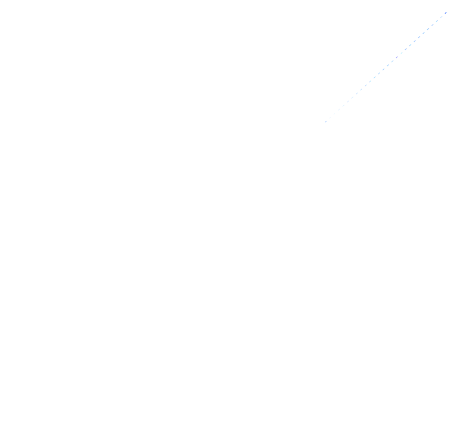
\includegraphics[width=0.9\textwidth]{2023StAndrewsAstro/Figures/fluidelement.png}
\begin{itemize}
    \item Directly modelled
    \item Kinetic, Magnetic, thermal
\end{itemize}
\end{column}
\begin{column}{0.3\textwidth}
\centering
\textbf{Ionisation/excitation energy}
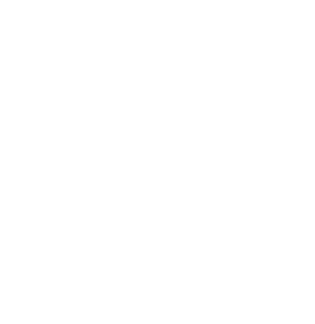
\includegraphics[width=0.8\textwidth]{2023StAndrewsAstro/Figures/ionenergy.png}
\begin{itemize}
    \item Not directly modelled but can be calculated
    \item Non-conservative 
    \item Energy remains 'in the system'.
\end{itemize}
\end{column}
\begin{column}{0.3\textwidth}
\centering
\textbf{Radiative energy}
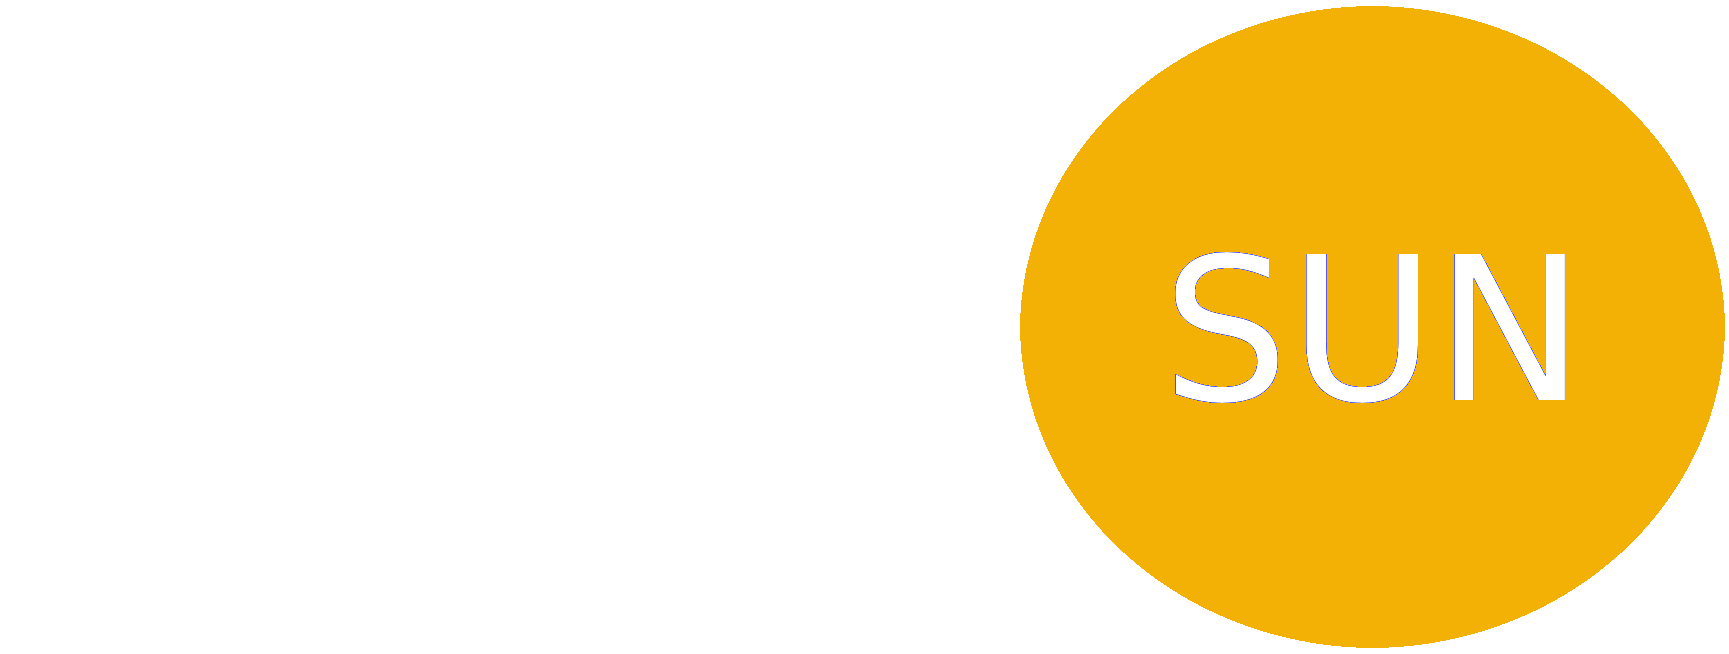
\includegraphics[width=0.8\textwidth]{2023StAndrewsAstro/Figures/radiationenergy.png}
\begin{itemize}
    \item Blackbody radiation field
    \item Not directly modelled/calculable 
    \item Allows energy to leave/enter the system
\end{itemize}
\end{column}
\end{columns}
\end{frame}

\begin{frame}{Collisional ionisation/recombination}
\begin{columns}
\begin{column}{0.4\textwidth}
\begin{enumerate}
\item Collisional ionisation only.
\item Shocks are highly dynamic and can have large temperature jumps.
\item Need to account for ionisation and recombination.
\item Kinetic energy of a free electron used to release a bound electron during ionisation.
\item Broadly used model for ionisation in two-fluid solar codes (AMRVAC, MANCHA, PIP)
\end{enumerate}
\end{column}
\begin{column}{0.6\textwidth}
Empirical rates for hydrogen from Voranov (1997) and Smirnov (2003) in normalised form:
    \begin{gather}
    \Gamma_{rec} = \frac{\rho_{\rm p}}{\sqrt{T_{\rm p}}} \frac{\sqrt{T_f}}{\xi _{{\rm p}0}} \tau _{IR} = F(T) \rho_{\rm p}, \\
    \Gamma_{ion} = \rho_{\rm p} \frac{\mbox{e} ^{-\chi} \chi ^{0.39} }{0.232 + \chi} \frac{\hat{R}}{\xi _{{\rm p}0}} \tau _{IR} = G(T) \rho_{\rm p}, \\
    \chi = 13.6 \frac{T_f}{T_{e0} T_{\rm p}}, \\
    \hat{R} = \frac{2.91 \times 10 ^{-14}}{2.6 \times 10^{-19}} \sqrt{T_{e0}},
    %\\ T_f = \frac{1}{4} \beta \gamma \frac{2 \xi_{p0}}{\xi_{n0} +2 \xi_{p0}}
\end{gather}
\end{column}
\end{columns}
\end{frame}

\begin{frame}{Equilibrium conditions - IRIP model}
\textbf{Ionisation, recombination and ionisation potential equilibrium conditions}
\begin{columns}
\begin{column}{0.45\textwidth}
\begin{figure}
    \centering
    % 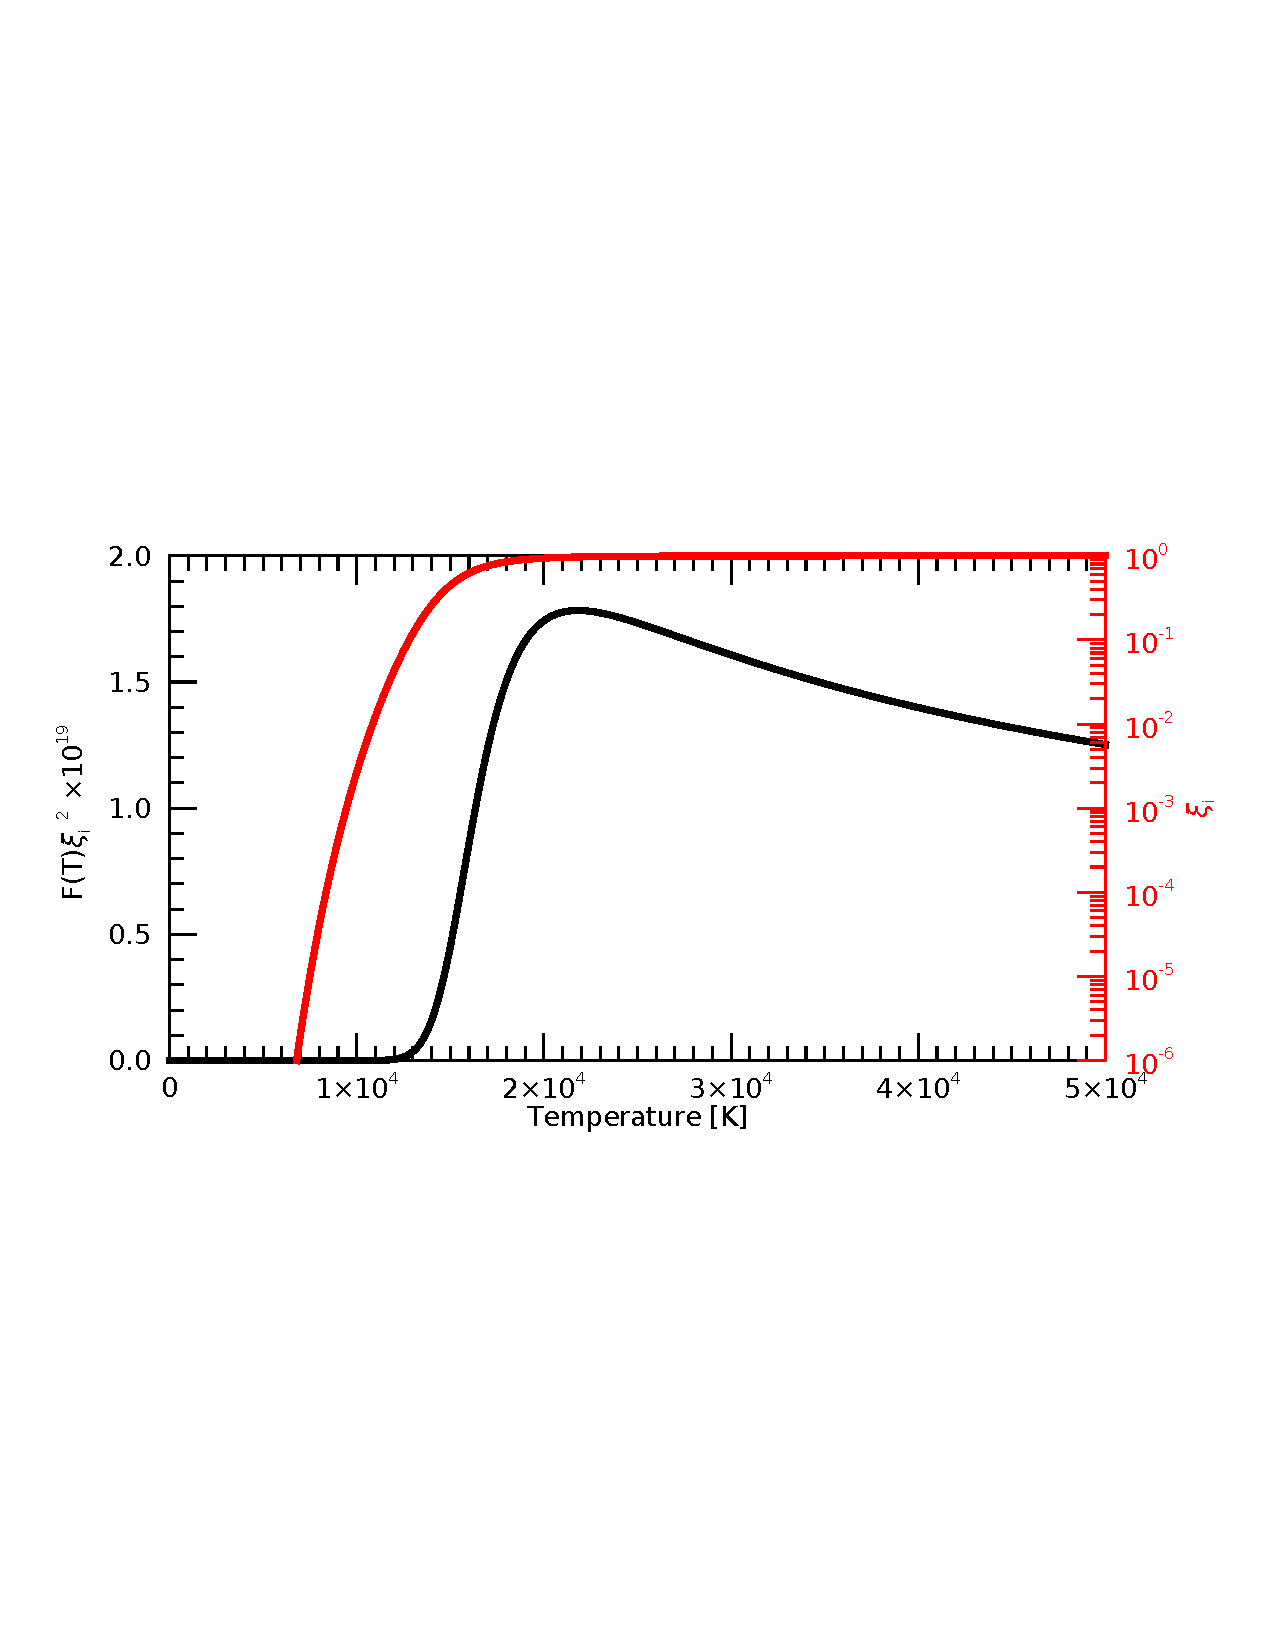
\includegraphics[width=0.95\linewidth,clip=true,trim=0.9cm 8.8cm 0.9cm 8.8cm]{2023StAndrews/Figures/eqltest3.pdf} \\
    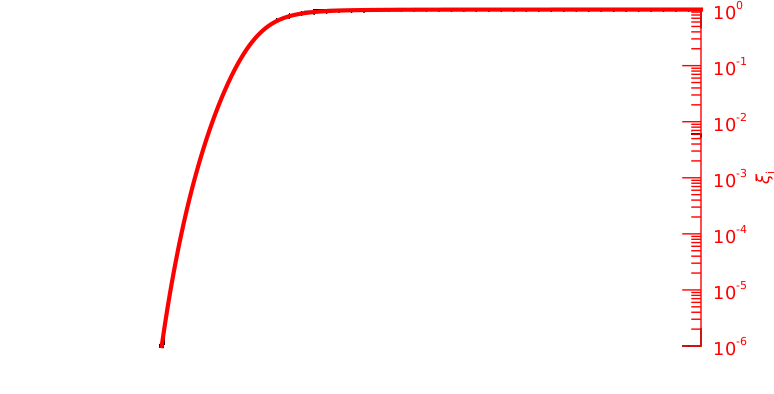
\includegraphics[width=0.95\linewidth]{2023StAndrewsAstro/Figures/eqltest3.png} \\
    % \caption{$F(T) \xi_i^2$ as a function of temperature in dimensional form. Red line shows the ionisation fraction $\xi_i$ for the associated temperature.}
    % \label{fig:eqltest}
    % 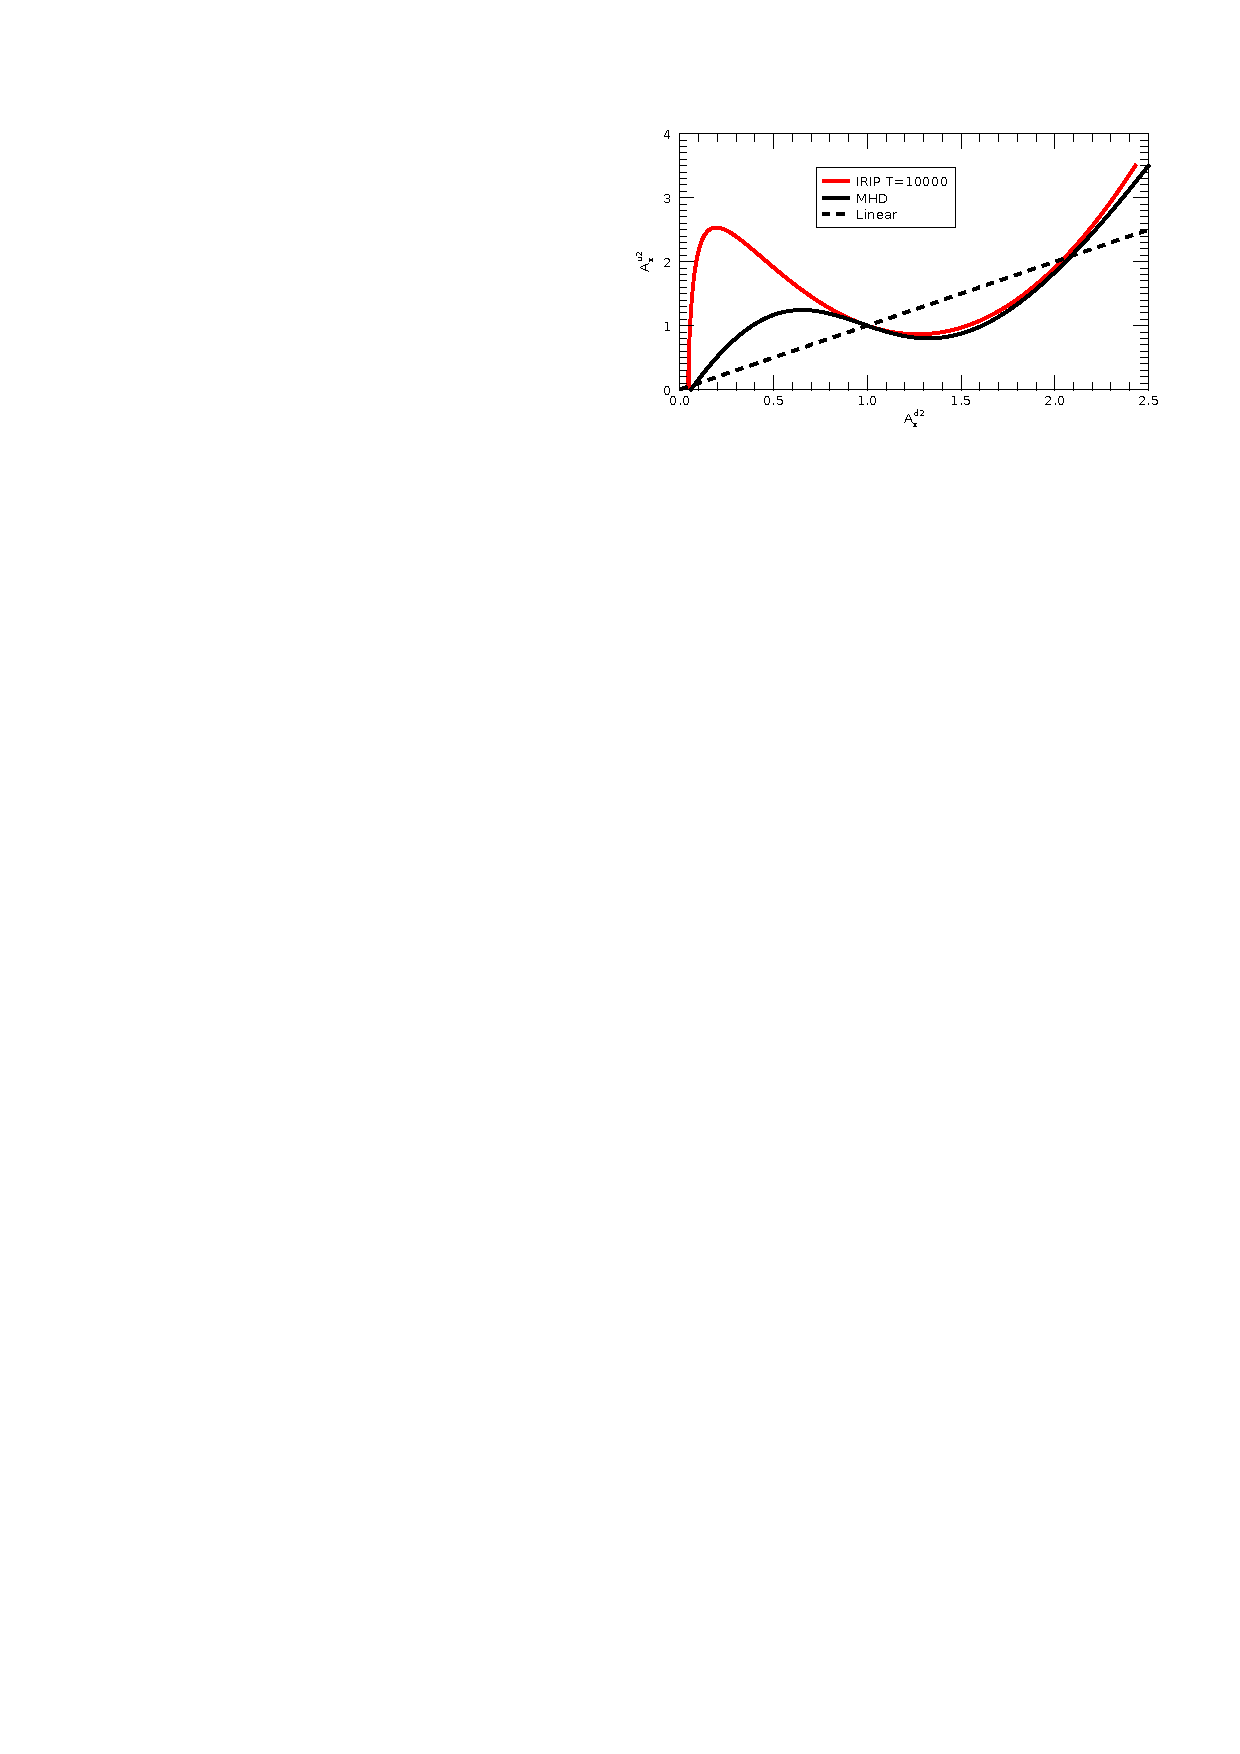
\includegraphics[width=0.95\linewidth]{2023DundeeInterview/Figures/aa39667-20-fig2.pdf}
    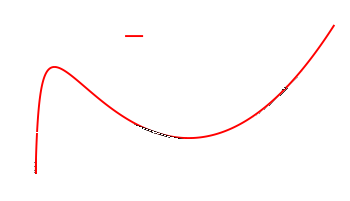
\includegraphics[width=0.95\linewidth]{2023StAndrewsAstro/Figures/aa39667-20-fig2.png}
\end{figure}
\end{column}
\begin{column}{0.55\textwidth}
Including the ionisation potential for an equilibrium, we require that the ionisation potential and heating terms balance:
\begin{gather}
    \hat{\phi} \Gamma _{ion} \rho_{\rm n} = \hat{\phi} \Gamma _{ion} (t=0) \rho _{\rm n} (t=0), \\
    \Gamma _{ion} \rho_{\rm n} = \Gamma _{rec} \rho_{\rm p} = \Gamma _{ion} (t=0) \rho _{\rm n} (t=0) =\mbox{const.} \\
    G(T)\rho_{\rm p} \rho_{\rm n} = F(T) \rho_{\rm p} ^2 = \mbox{const.} \\
    F(T) \xi_i ^2 \rho ^2 = \mbox{const.} \\
     \xi_i=\frac{1}{\frac{F(T)}{G(T)} +1}.
\end{gather}
\textbf{A compressible partially-ionised shock must cool across the interface!}
\end{column}
\end{columns}
\end{frame}

\begin{frame}{IRIP model}
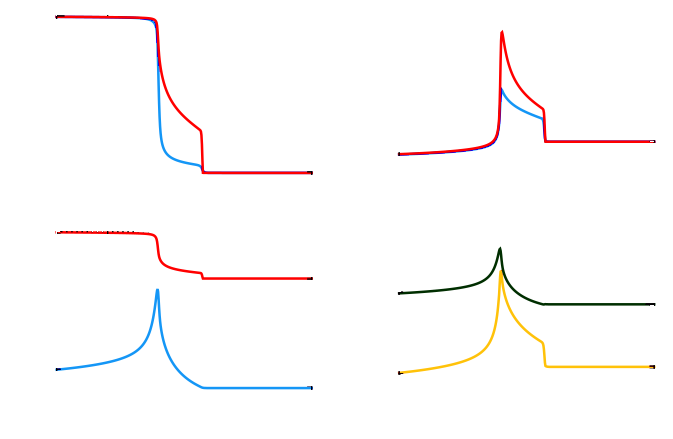
\includegraphics[width=0.85\textwidth]{2023StAndrewsAstro/Figures/irip_shock.png}
\end{frame}

\begin{frame}{Problems}
\begin{columns}
\begin{column}{0.4\textwidth}
\begin{itemize}
%\item Two-fluid model - ion+electron plasma, and bulk neutral fluid.
\item This implies shocks cool rather than heat! (Snow+2021)
\item Similar cooling solutions in corona-like radiative MHD model (Snow2023/2024, in prep)  
\item Empirical rates are fitted to data warmer than the chromosphere
\item No radiation
\item All ionisation comes from ground state
\end{itemize}
\end{column}
\begin{column}{0.6\textwidth}
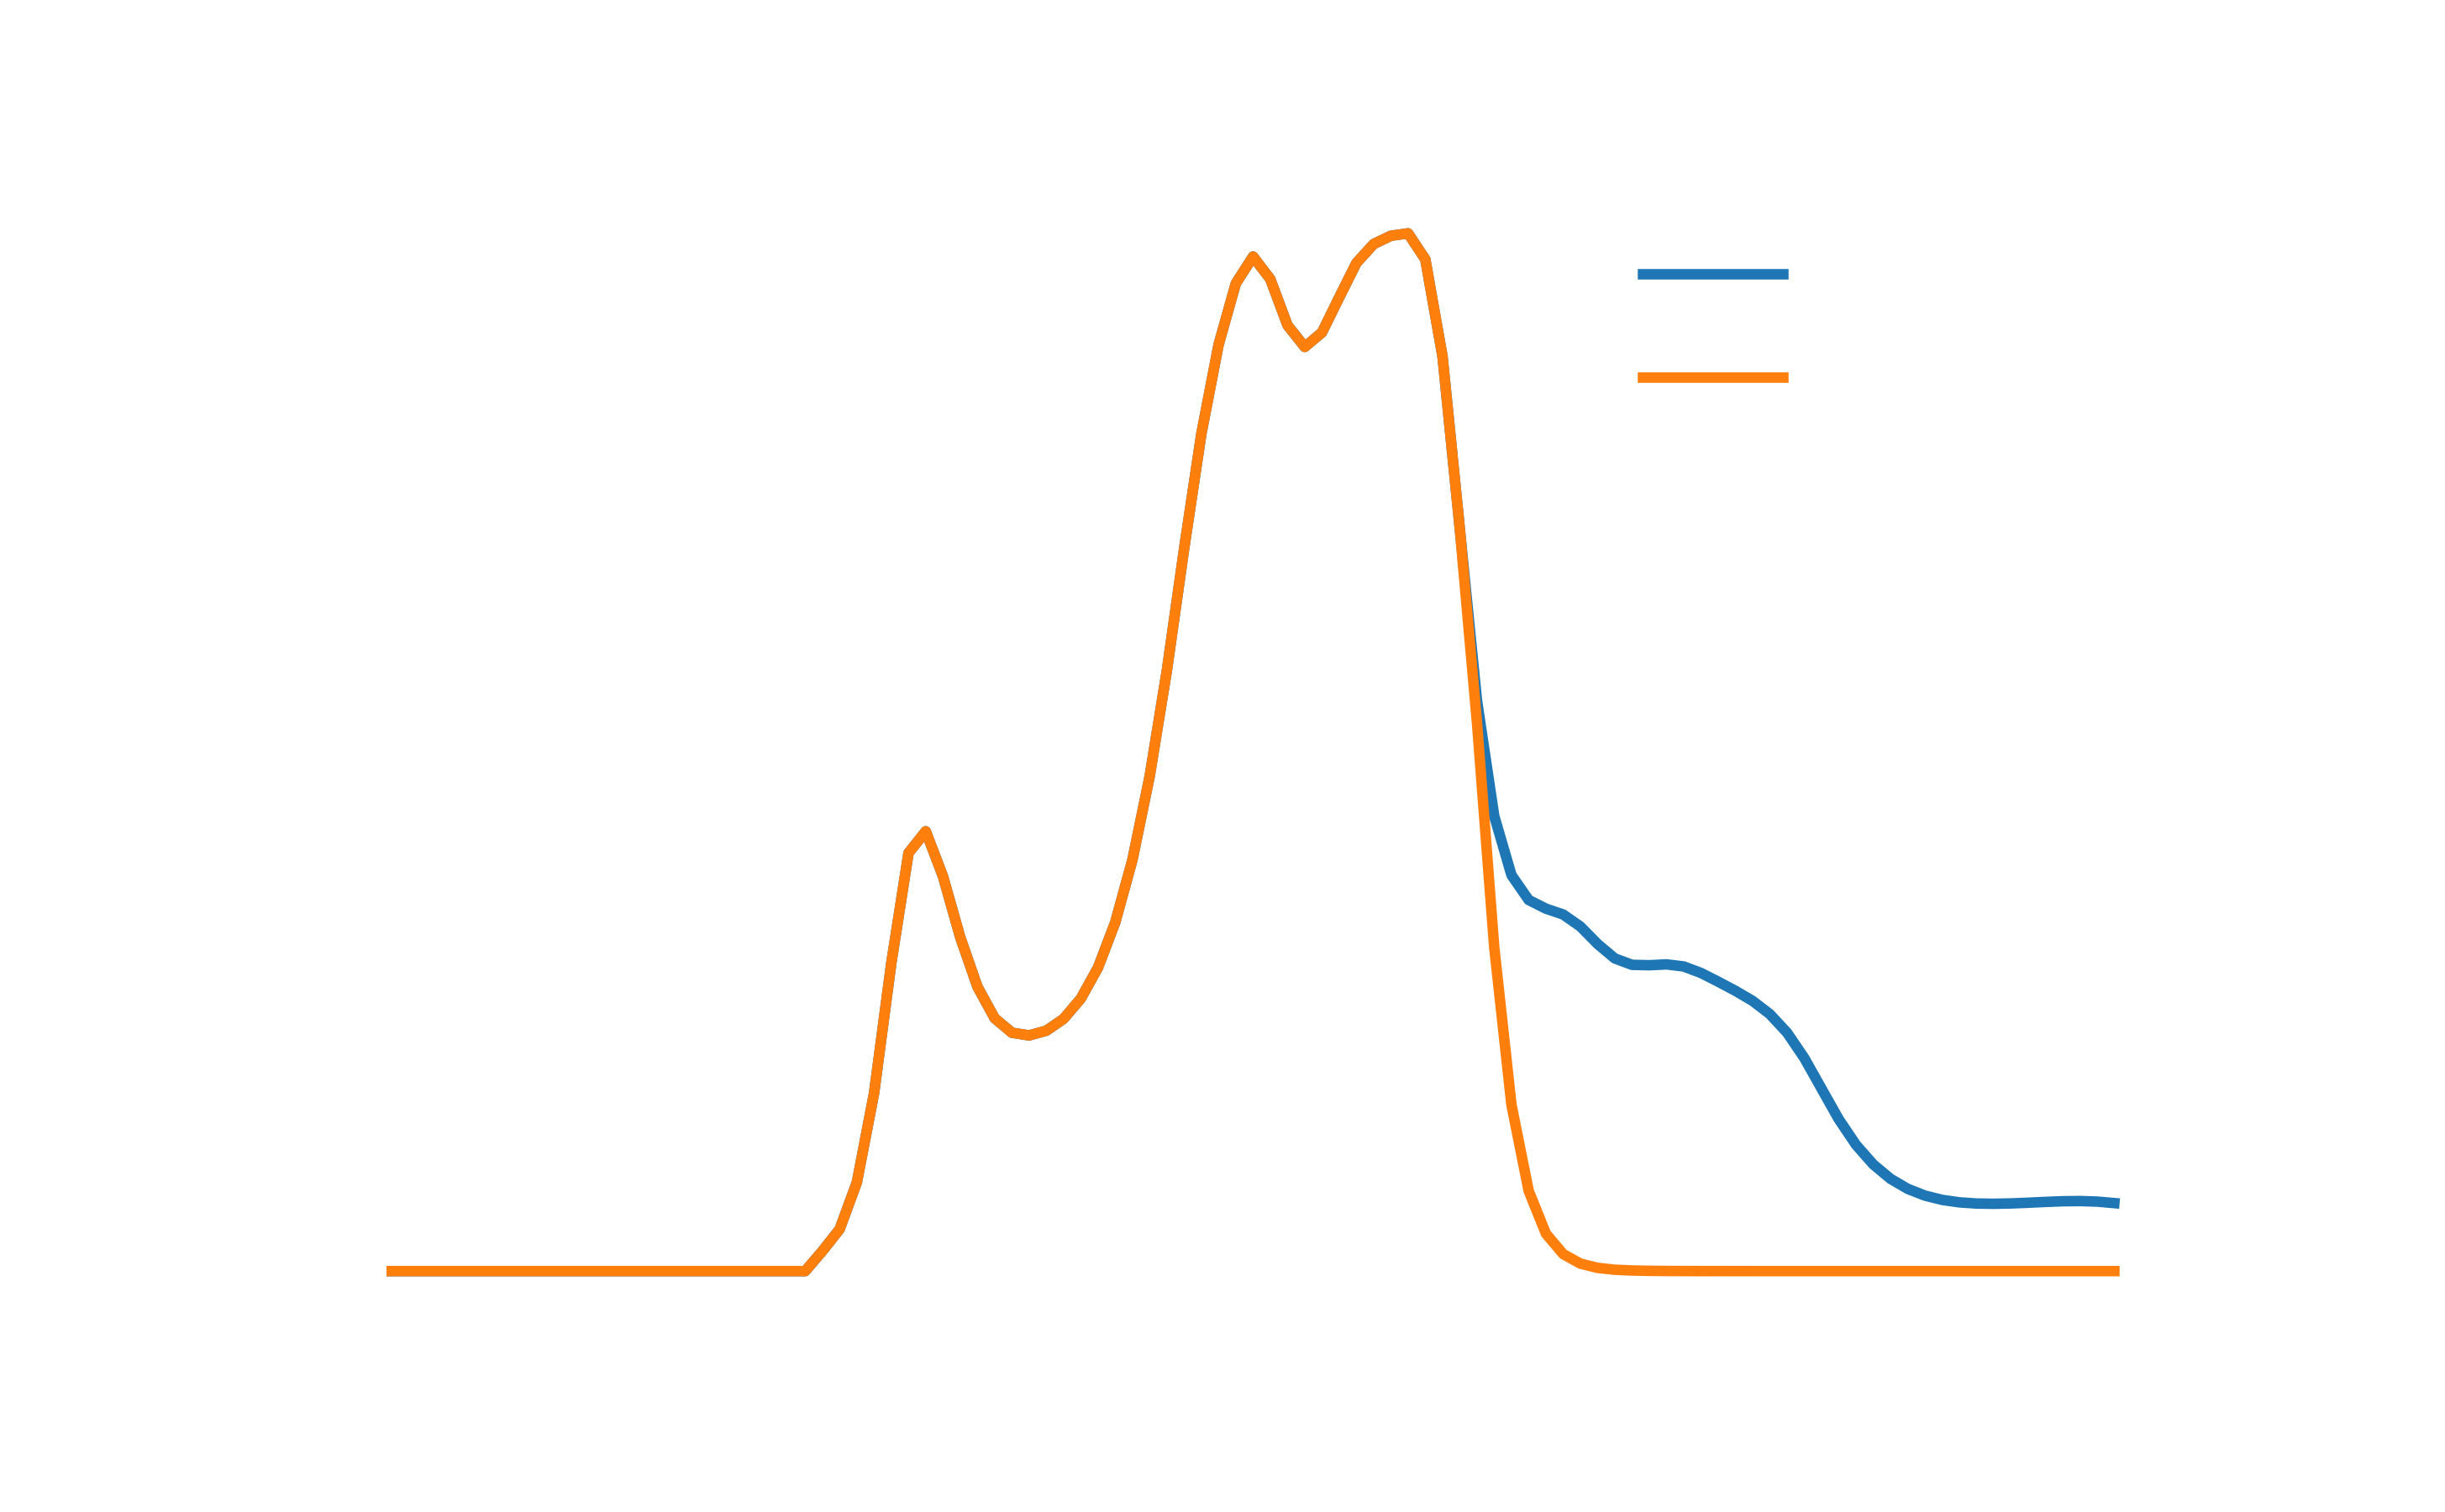
\includegraphics[width=0.9\linewidth]{2023StAndrewsAstro/Figures/KHIrl2D_lossprofile.png}
\begin{itemize}
%\item Two-fluid model - ion+electron plasma, and bulk neutral fluid.
\item Need more comprehensive model! Needs collisional and radiative rates. Self-consistent heating terms, etc.... 
\item Developed multi-level hydrogen model - offers unparalleled treatment of partial ionisation (Snow+2023)
\end{itemize}
\end{column}
\end{columns}
\end{frame}

% \begin{frame}{Partially ionised plasma}
% \begin{columns}
% \begin{column}{0.5\textwidth}
% \begin{itemize}
%     \item State-of-the-art - use empirical models for ionisation/recombination
%     \item Equations become non-conservative
%     \item Allows for (semi-)analytical models for the shock jumps 
% \end{itemize}
% \end{column}
% \begin{column}{0.5\textwidth}
% %\includegraphics[width=0.32\linewidth]{Figures/Crab_Nebula.jpeg}
% %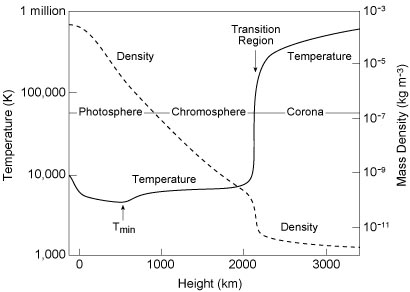
\includegraphics[width=0.95\linewidth]{2023Dundee/Figures/valc.png} \\
% %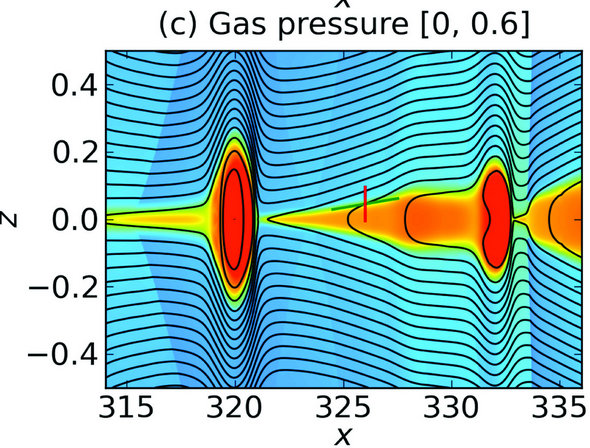
\includegraphics[width=0.95\linewidth]{2023RAS/Figures/shibyama.png}
% %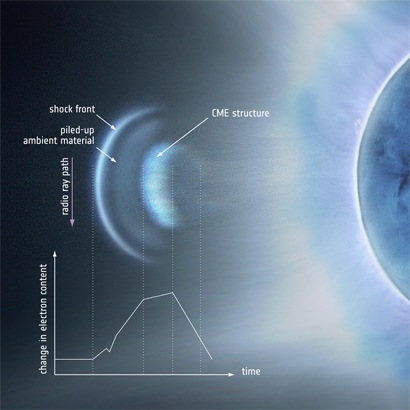
\includegraphics[width=0.32\linewidth]{Figures/cmesketch.jpg}
% \end{column}
% \end{columns}
% \end{frame}

% \begin{frame}{Partially ionised plasma - equilibrium conditions}
% \begin{columns}
% \begin{column}{0.5\textwidth}
% \begin{itemize}
%     \item Shocks (which are compressional) necessarily cool!
%     \item 
% \end{itemize}
% \end{column}
% \begin{column}{0.5\textwidth}
% %\includegraphics[width=0.32\linewidth]{Figures/Crab_Nebula.jpeg}
% %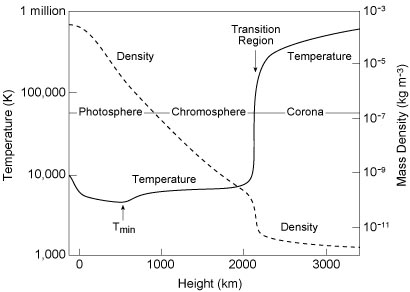
\includegraphics[width=0.95\linewidth]{2023Dundee/Figures/valc.png} \\
% %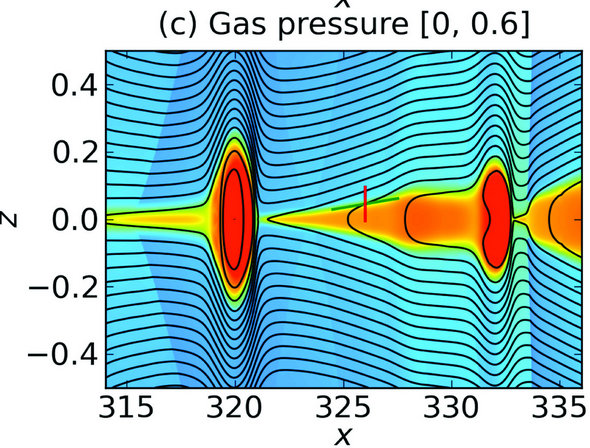
\includegraphics[width=0.95\linewidth]{2023RAS/Figures/shibyama.png}
% %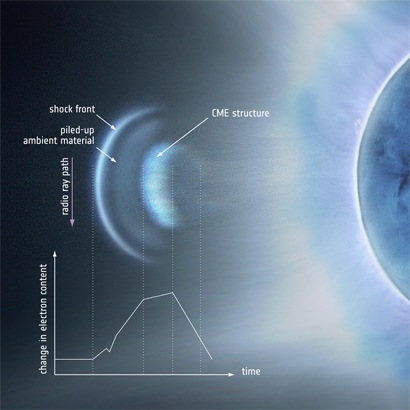
\includegraphics[width=0.32\linewidth]{Figures/cmesketch.jpg}
% \end{column}
% \end{columns}
% \end{frame}

% \begin{frame}{Problem}
% \begin{columns}
% \begin{column}{0.5\textwidth}
% \begin{itemize}
%     \item Ionisation/recombination models are empirical fits to data not in the range (extrapolation)
%     \item Heating term is anomalous 
%     \item Ionisation from ground state - overprediction of losses
%     \item Radiative field
% \end{itemize}
% \end{column}
% \begin{column}{0.5\textwidth}
% %\includegraphics[width=0.32\linewidth]{Figures/Crab_Nebula.jpeg}
% %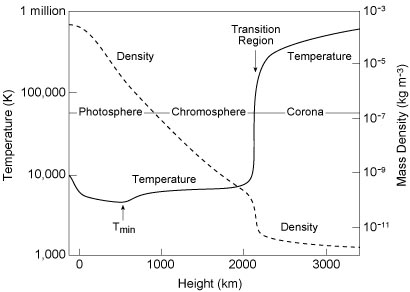
\includegraphics[width=0.95\linewidth]{2023Dundee/Figures/valc.png} \\
% %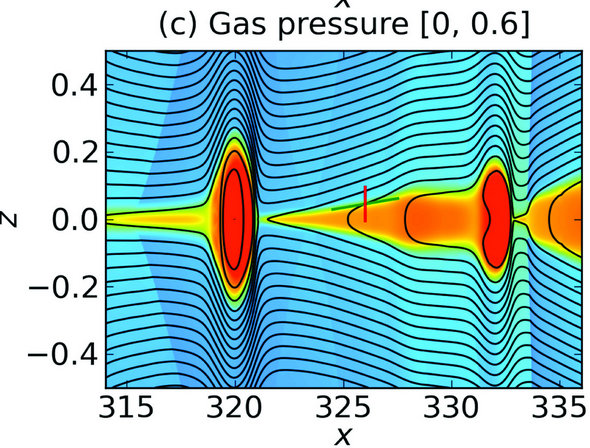
\includegraphics[width=0.95\linewidth]{2023RAS/Figures/shibyama.png}
% %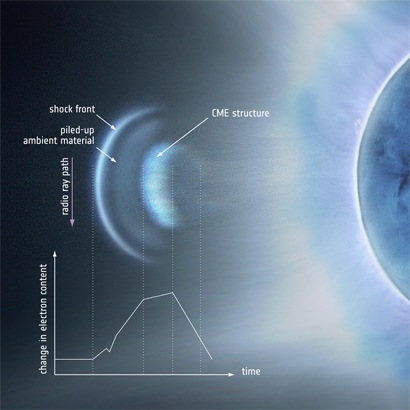
\includegraphics[width=0.32\linewidth]{Figures/cmesketch.jpg}
% \end{column}
% \end{columns}
% \end{frame}

% \begin{frame}{Solutions}
% \begin{columns}
% \begin{column}{0.5\textwidth}
% \begin{itemize}
%     \item Multi-level collisional and radiative two-fluid model
%     \item Self-consistent heating
%     \item What is the thermal contribution of shocks?
% \end{itemize}
% \end{column}
% \begin{column}{0.5\textwidth}
% %\includegraphics[width=0.32\linewidth]{Figures/Crab_Nebula.jpeg}
% %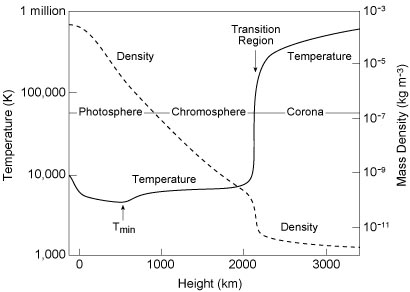
\includegraphics[width=0.95\linewidth]{2023Dundee/Figures/valc.png} \\
% %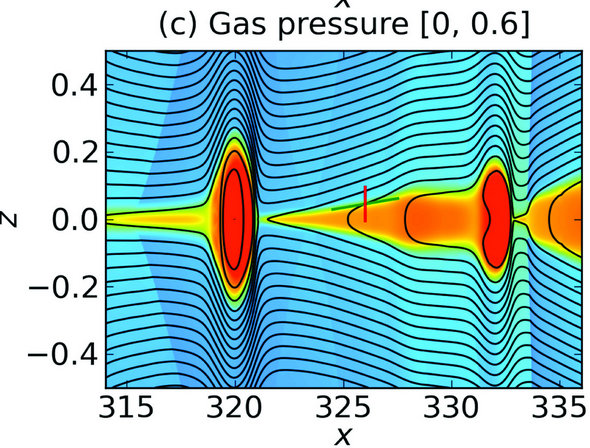
\includegraphics[width=0.95\linewidth]{2023RAS/Figures/shibyama.png}
% %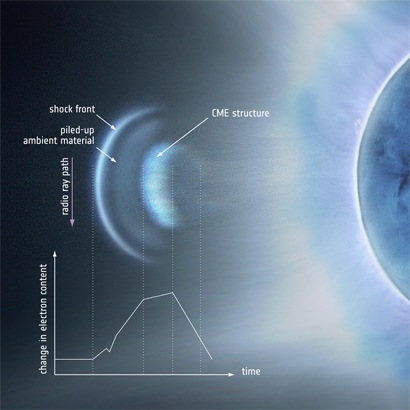
\includegraphics[width=0.32\linewidth]{Figures/cmesketch.jpg}
% \end{column}
% \end{columns}
% \end{frame}

%%%%%%%%%%%%%%%%%%%%%%%%%%%%%%%%%%%%%%%%%%%%%%%%%%%%%%%%%%%%%%%%%%%%%%%%%%%%%%%%%%

% \begin{frame}{Ionisation, recombination and ionisation potential in two-fluid shocks}
% \footnotesize
% \begin{gather}
% \frac{\partial \rho _{\text{n}}}{\partial t} + \nabla \cdot (\rho _{\text{n}} \textbf{v}_{\text{n}})= \Gamma _{rec} \rho _{\rm p} - \Gamma _{ion} \rho _{\rm n}, \label{eqn:neutral1}\tag{5} \\
% \frac{\partial}{\partial t}(\rho _{\text{n}} \textbf{v}_{\text{n}}) + \nabla \cdot (\rho _{\text{n}} \textbf{v}_{\text{n}} \textbf{v}_{\text{n}} + P_{\text{n}} \textbf{I}) = -\alpha _c \rho_{\text{n}} \rho_{\text{p}} (\textbf{v}_{\text{n}}-\textbf{v}_{\text{p}}) + \Gamma _{rec} \rho _{\rm p} \textbf{v}_{\rm p} - \Gamma _{ion} \rho_{\rm n} \textbf{v}_{\rm n}, \tag{6}\\
% \frac{\partial e_{\text{n}}}{\partial t} + \nabla \cdot \left[\textbf{v}_{\text{n}} (e_{\text{n}} +P_{\text{n}}) \right] = -\alpha _c \rho _{\text{n}} \rho _{\text{p}} \left[ \frac{1}{2} (\textbf{v}_{\text{n}} ^2 - \textbf{v}_{\text{p}} ^2)+ \frac{3}{2} \left(\frac{P_{\rm n}}{\rho_{\rm n}}-\frac{1}{2}\frac{P_{\rm p}}{\rho_{\rm p}}\right) \right] \nonumber \\ \hspace{0.5cm}+ \frac{1}{2} \left( \Gamma _{rec} \rho _{\rm p} \textbf{v}_{\rm p} ^2 - \Gamma _{ion} \rho _{\rm n} \textbf{v}_{\rm n} ^2 \right) +\frac{1}{ (\gamma-1)} \left( \frac{1}{2} \Gamma _{rec} P_{\rm p} -\Gamma _{ion} P_{\rm n} \right), \tag{7}\\
% %e_{\text{n}} = \frac{P_{\text{n}}}{\gamma -1} + \frac{1}{2} \rho _{\text{n}} v_{\text{n}} ^2, \label{eqn:neutral2} \\
% \frac{\partial \rho _{\text{p}}}{\partial t} + \nabla \cdot (\rho_{\text{p}} \textbf{v}_{\text{p}}) = - \Gamma _{rec} \rho _{\rm p} + \Gamma _{ion} \rho _{\rm n} \label{eqn:plasma1}\tag{8}\\
% \frac{\partial}{\partial t} (\rho_{\text{p}} \textbf{v}_{\text{p}})+ \nabla \cdot \left( \rho_{\text{p}} \textbf{v}_{\text{p}} \textbf{v}_{\text{p}} + P_{\text{p}} \textbf{I} - \textbf{B B} + \frac{\textbf{B}^2}{2} \textbf{I} \right) = \alpha _c \rho_{\text{n}} \rho_{\text{p}}(\textbf{v}_{\text{n}} - \textbf{v}_{\text{p}}) - \Gamma _{rec} \rho _{\rm p} \textbf{v}_{\rm p} + \Gamma _{ion} \rho_{\rm n} \textbf{v}_{\rm n},\tag{9}\\
% \frac{\partial}{\partial t} \left( e_{\text{p}} + \frac{\textbf{B}^2}{2} \right) + \nabla \cdot \left[ \textbf{v}_{\text{p}} ( e_{\text{p}} + P_{\text{p}}) -  (\textbf{v}_{\rm p} \times \textbf{B}) \times \textbf{B} \right]  =  \alpha _c \rho _{\text{n}} \rho _{\text{p}} \left[ \frac{1}{2} (\textbf{v}_{\text{n}} ^2 - \textbf{v}_{\text{p}} ^2)+ \frac{3}{2} \left(\frac{P_{\rm n}}{\rho_{\rm n}}-\frac{1}{2}\frac{P_{\rm p}}{\rho_{\rm p}}\right) \right] \nonumber \\ \hspace{0.5cm}- \frac{1}{2} \left( \Gamma _{rec} \rho _{\rm p} \textbf{v}_{\rm p} ^2 - \Gamma _{ion} \rho _{\rm n} \textbf{v}_{\rm n} ^2 \right) {- \phi_I + \phi_{heat}} -\frac{1}{ (\gamma-1)} \left( \frac{1}{2} \Gamma _{rec} P_{\rm p} -\Gamma _{ion} P_{\rm n} \right), \label{eqn:ep}\tag{10} \\
% \frac{\partial \textbf{B}}{\partial t} - \nabla \times (\textbf{v}_{\text{p}} \times \textbf{B}) = 0.\tag{11}
% %e_{\text{p}} = \frac{P_{\text{p}}}{\gamma -1} + \frac{1}{2} \rho _{\text{p}} v_{\text{p}} ^2, \\
% %\nabla \cdot \textbf{B} = 0,\label{eqn:plasma2}
% \end{gather}
% \end{frame}

% \begin{frame}{Ionisation, recombination and ionisation potential in two-fluid shocks}
% \vspace{-0.5cm}
% \footnotesize
% \begin{gather}
% \mathcolorbox{VioletRed}{\frac{\partial \rho _{\text{n}}}{\partial t} + \nabla \cdot (\rho _{\text{n}} \textbf{v}_{\text{n}})}= \Gamma _{rec} \rho _{\rm p} - \Gamma _{ion} \rho _{\rm n}, \label{eqn:neutral1}\tag{5} \\
% \mathcolorbox{VioletRed}{\frac{\partial}{\partial t}(\rho _{\text{n}} \textbf{v}_{\text{n}}) + \nabla \cdot (\rho _{\text{n}} \textbf{v}_{\text{n}} \textbf{v}_{\text{n}} + P_{\text{n}} \textbf{I})} = -\alpha _c \rho_{\text{n}} \rho_{\text{p}} (\textbf{v}_{\text{n}}-\textbf{v}_{\text{p}}) + \Gamma _{rec} \rho _{\rm p} \textbf{v}_{\rm p} - \Gamma _{ion} \rho_{\rm n} \textbf{v}_{\rm n}, \tag{6}\\
% \mathcolorbox{VioletRed}{\frac{\partial e_{\text{n}}}{\partial t} + \nabla \cdot \left[\textbf{v}_{\text{n}} (e_{\text{n}} +P_{\text{n}}) \right]} = -\alpha _c \rho _{\text{n}} \rho _{\text{p}} \left[ \frac{1}{2} (\textbf{v}_{\text{n}} ^2 - \textbf{v}_{\text{p}} ^2)+ \frac{3}{2} \left(\frac{P_{\rm n}}{\rho_{\rm n}}-\frac{1}{2}\frac{P_{\rm p}}{\rho_{\rm p}}\right) \right] \nonumber \\ \hspace{0.5cm}+ \frac{1}{2} \left( \Gamma _{rec} \rho _{\rm p} \textbf{v}_{\rm p} ^2 - \Gamma _{ion} \rho _{\rm n} \textbf{v}_{\rm n} ^2 \right) +\frac{1}{ (\gamma-1)} \left( \frac{1}{2} \Gamma _{rec} P_{\rm p} -\Gamma _{ion} P_{\rm n} \right), \tag{7}\\
% %e_{\text{n}} = \frac{P_{\text{n}}}{\gamma -1} + \frac{1}{2} \rho _{\text{n}} v_{\text{n}} ^2, \label{eqn:neutral2} \\
% \frac{\partial \rho _{\text{p}}}{\partial t} + \nabla \cdot (\rho_{\text{p}} \textbf{v}_{\text{p}}) = - \Gamma _{rec} \rho _{\rm p} + \Gamma _{ion} \rho _{\rm n} \label{eqn:plasma1}\tag{8}\\
% \frac{\partial}{\partial t} (\rho_{\text{p}} \textbf{v}_{\text{p}})+ \nabla \cdot \left( \rho_{\text{p}} \textbf{v}_{\text{p}} \textbf{v}_{\text{p}} + P_{\text{p}} \textbf{I} - \textbf{B B} + \frac{\textbf{B}^2}{2} \textbf{I} \right) = \alpha _c \rho_{\text{n}} \rho_{\text{p}}(\textbf{v}_{\text{n}} - \textbf{v}_{\text{p}}) - \Gamma _{rec} \rho _{\rm p} \textbf{v}_{\rm p} + \Gamma _{ion} \rho_{\rm n} \textbf{v}_{\rm n},\tag{9}\\
% \frac{\partial}{\partial t} \left( e_{\text{p}} + \frac{\textbf{B}^2}{2} \right) + \nabla \cdot \left[ \textbf{v}_{\text{p}} ( e_{\text{p}} + P_{\text{p}}) -  (\textbf{v}_{\rm p} \times \textbf{B}) \times \textbf{B} \right]  =  \alpha _c \rho _{\text{n}} \rho _{\text{p}} \left[ \frac{1}{2} (\textbf{v}_{\text{n}} ^2 - \textbf{v}_{\text{p}} ^2)+ \frac{3}{2} \left(\frac{P_{\rm n}}{\rho_{\rm n}}-\frac{1}{2}\frac{P_{\rm p}}{\rho_{\rm p}}\right) \right] \nonumber \\ \hspace{0.5cm}- \frac{1}{2} \left( \Gamma _{rec} \rho _{\rm p} \textbf{v}_{\rm p} ^2 - \Gamma _{ion} \rho _{\rm n} \textbf{v}_{\rm n} ^2 \right) {- \phi_I + \phi_{heat}} -\frac{1}{ (\gamma-1)} \left( \frac{1}{2} \Gamma _{rec} P_{\rm p} -\Gamma _{ion} P_{\rm n} \right), \label{eqn:ep} \tag{10}\\
% \frac{\partial \textbf{B}}{\partial t} - \nabla \times (\textbf{v}_{\text{p}} \times \textbf{B}) = 0.\tag{11}
% %e_{\text{p}} = \frac{P_{\text{p}}}{\gamma -1} + \frac{1}{2} \rho _{\text{p}} v_{\text{p}} ^2, \\
% %\nabla \cdot \textbf{B} = 0,\label{eqn:plasma2}
% \end{gather}
% \end{frame}

% \begin{frame}{Ionisation, recombination and ionisation potential in two-fluid shocks}
% \vspace{-0.5cm}
% \footnotesize
% \begin{gather}
% \frac{\partial \rho _{\text{n}}}{\partial t} + \nabla \cdot (\rho _{\text{n}} \textbf{v}_{\text{n}})= \Gamma _{rec} \rho _{\rm p} - \Gamma _{ion} \rho _{\rm n}, \label{eqn:neutral1}\tag{5} \\
% \frac{\partial}{\partial t}(\rho _{\text{n}} \textbf{v}_{\text{n}}) + \nabla \cdot (\rho _{\text{n}} \textbf{v}_{\text{n}} \textbf{v}_{\text{n}} + P_{\text{n}} \textbf{I}) = -\alpha _c \rho_{\text{n}} \rho_{\text{p}} (\textbf{v}_{\text{n}}-\textbf{v}_{\text{p}}) + \Gamma _{rec} \rho _{\rm p} \textbf{v}_{\rm p} - \Gamma _{ion} \rho_{\rm n} \textbf{v}_{\rm n}, \tag{6}\\
% \frac{\partial e_{\text{n}}}{\partial t} + \nabla \cdot \left[\textbf{v}_{\text{n}} (e_{\text{n}} +P_{\text{n}}) \right] = -\alpha _c \rho _{\text{n}} \rho _{\text{p}} \left[ \frac{1}{2} (\textbf{v}_{\text{n}} ^2 - \textbf{v}_{\text{p}} ^2)+ \frac{3}{2} \left(\frac{P_{\rm n}}{\rho_{\rm n}}-\frac{1}{2}\frac{P_{\rm p}}{\rho_{\rm p}}\right) \right] \nonumber \\ \hspace{0.5cm}+ \frac{1}{2} \left( \Gamma _{rec} \rho _{\rm p} \textbf{v}_{\rm p} ^2 - \Gamma _{ion} \rho _{\rm n} \textbf{v}_{\rm n} ^2 \right) +\frac{1}{ (\gamma-1)} \left( \frac{1}{2} \Gamma _{rec} P_{\rm p} -\Gamma _{ion} P_{\rm n} \right), \tag{7}\\
% %e_{\text{n}} = \frac{P_{\text{n}}}{\gamma -1} + \frac{1}{2} \rho _{\text{n}} v_{\text{n}} ^2, \label{eqn:neutral2} \\
% \mathcolorbox{BlueGreen}{\frac{\partial \rho _{\text{p}}}{\partial t} + \nabla \cdot (\rho_{\text{p}} \textbf{v}_{\text{p}})} = - \Gamma _{rec} \rho _{\rm p} + \Gamma _{ion} \rho _{\rm n} \label{eqn:plasma1}\tag{8}\\
% \mathcolorbox{BlueGreen}{\frac{\partial}{\partial t} (\rho_{\text{p}} \textbf{v}_{\text{p}})+ \nabla \cdot \left( \rho_{\text{p}} \textbf{v}_{\text{p}} \textbf{v}_{\text{p}} + P_{\text{p}} \textbf{I} - \textbf{B B} + \frac{\textbf{B}^2}{2} \textbf{I} \right)} = \alpha _c \rho_{\text{n}} \rho_{\text{p}}(\textbf{v}_{\text{n}} - \textbf{v}_{\text{p}}) - \Gamma _{rec} \rho _{\rm p} \textbf{v}_{\rm p} + \Gamma _{ion} \rho_{\rm n} \textbf{v}_{\rm n},\tag{9}\\
% \mathcolorbox{BlueGreen}{\frac{\partial}{\partial t} \left( e_{\text{p}} + \frac{\textbf{B}^2}{2} \right) + \nabla \cdot \left[ \textbf{v}_{\text{p}} ( e_{\text{p}} + P_{\text{p}}) -  (\textbf{v}_{\rm p} \times \textbf{B}) \times \textbf{B} \right] } =  \alpha _c \rho _{\text{n}} \rho _{\text{p}} \left[ \frac{1}{2} (\textbf{v}_{\text{n}} ^2 - \textbf{v}_{\text{p}} ^2)+ \frac{3}{2} \left(\frac{P_{\rm n}}{\rho_{\rm n}}-\frac{1}{2}\frac{P_{\rm p}}{\rho_{\rm p}}\right) \right] \nonumber \\ \hspace{0.5cm}- \frac{1}{2} \left( \Gamma _{rec} \rho _{\rm p} \textbf{v}_{\rm p} ^2 - \Gamma _{ion} \rho _{\rm n} \textbf{v}_{\rm n} ^2 \right) {- \phi_I + \phi_{heat}} -\frac{1}{ (\gamma-1)} \left( \frac{1}{2} \Gamma _{rec} P_{\rm p} -\Gamma _{ion} P_{\rm n} \right), \label{eqn:ep}\tag{10} \\
% \mathcolorbox{BlueGreen}{\frac{\partial \textbf{B}}{\partial t} - \nabla \times (\textbf{v}_{\text{p}} \times \textbf{B}) = 0.}\tag{11}
% %e_{\text{p}} = \frac{P_{\text{p}}}{\gamma -1} + \frac{1}{2} \rho _{\text{p}} v_{\text{p}} ^2, \\
% %\nabla \cdot \textbf{B} = 0,\label{eqn:plasma2}
% \end{gather}
% \end{frame}

% \begin{frame}{Ionisation, recombination and ionisation potential in two-fluid shocks}
% \vspace{-0.5cm}
% \footnotesize
% \begin{gather}
% \frac{\partial \rho _{\text{n}}}{\partial t} + \nabla \cdot (\rho _{\text{n}} \textbf{v}_{\text{n}})= \Gamma _{rec} \rho _{\rm p} - \Gamma _{ion} \rho _{\rm n}, \label{eqn:neutral1}\tag{5} \\
% \frac{\partial}{\partial t}(\rho _{\text{n}} \textbf{v}_{\text{n}}) + \nabla \cdot (\rho _{\text{n}} \textbf{v}_{\text{n}} \textbf{v}_{\text{n}} + P_{\text{n}} \textbf{I}) =\mathcolorbox{YellowOrange}{ -\alpha _c \rho_{\text{n}} \rho_{\text{p}} (\textbf{v}_{\text{n}}-\textbf{v}_{\text{p}})} + \Gamma _{rec} \rho _{\rm p} \textbf{v}_{\rm p} - \Gamma _{ion} \rho_{\rm n} \textbf{v}_{\rm n}, \tag{6}\\
% \frac{\partial e_{\text{n}}}{\partial t} + \nabla \cdot \left[\textbf{v}_{\text{n}} (e_{\text{n}} +P_{\text{n}}) \right] = \mathcolorbox{YellowOrange}{-\alpha _c \rho _{\text{n}} \rho _{\text{p}} \left[ \frac{1}{2} (\textbf{v}_{\text{n}} ^2 - \textbf{v}_{\text{p}} ^2)+ \frac{3}{2} \left(\frac{P_{\rm n}}{\rho_{\rm n}}-\frac{1}{2}\frac{P_{\rm p}}{\rho_{\rm p}}\right) \right]} \nonumber \\ \hspace{0.5cm}+ \frac{1}{2} \left( \Gamma _{rec} \rho _{\rm p} \textbf{v}_{\rm p} ^2 - \Gamma _{ion} \rho _{\rm n} \textbf{v}_{\rm n} ^2 \right) +\frac{1}{ (\gamma-1)} \left( \frac{1}{2} \Gamma _{rec} P_{\rm p} -\Gamma _{ion} P_{\rm n} \right), \tag{7}\\
% %e_{\text{n}} = \frac{P_{\text{n}}}{\gamma -1} + \frac{1}{2} \rho _{\text{n}} v_{\text{n}} ^2, \label{eqn:neutral2} \\
% \frac{\partial \rho _{\text{p}}}{\partial t} + \nabla \cdot (\rho_{\text{p}} \textbf{v}_{\text{p}}) = - \Gamma _{rec} \rho _{\rm p} + \Gamma _{ion} \rho _{\rm n} \label{eqn:plasma1}\tag{8}\\
% \frac{\partial}{\partial t} (\rho_{\text{p}} \textbf{v}_{\text{p}})+ \nabla \cdot \left( \rho_{\text{p}} \textbf{v}_{\text{p}} \textbf{v}_{\text{p}} + P_{\text{p}} \textbf{I} - \textbf{B B} + \frac{\textbf{B}^2}{2} \textbf{I} \right) = \mathcolorbox{YellowOrange}{\alpha _c \rho_{\text{n}} \rho_{\text{p}}(\textbf{v}_{\text{n}} - \textbf{v}_{\text{p}})} - \Gamma _{rec} \rho _{\rm p} \textbf{v}_{\rm p} + \Gamma _{ion} \rho_{\rm n} \textbf{v}_{\rm n},\tag{9}\\
% \frac{\partial}{\partial t} \left( e_{\text{p}} + \frac{\textbf{B}^2}{2} \right) + \nabla \cdot \left[ \textbf{v}_{\text{p}} ( e_{\text{p}} + P_{\text{p}}) -  (\textbf{v}_{\rm p} \times \textbf{B}) \times \textbf{B} \right]  = \mathcolorbox{YellowOrange}{ \alpha _c \rho _{\text{n}} \rho _{\text{p}} \left[ \frac{1}{2} (\textbf{v}_{\text{n}} ^2 - \textbf{v}_{\text{p}} ^2)+ \frac{3}{2} \left(\frac{P_{\rm n}}{\rho_{\rm n}}-\frac{1}{2}\frac{P_{\rm p}}{\rho_{\rm p}}\right) \right]} \nonumber \\ \hspace{0.5cm}- \frac{1}{2} \left( \Gamma _{rec} \rho _{\rm p} \textbf{v}_{\rm p} ^2 - \Gamma _{ion} \rho _{\rm n} \textbf{v}_{\rm n} ^2 \right) {- \phi_I + \phi_{heat}} -\frac{1}{ (\gamma-1)} \left( \frac{1}{2} \Gamma _{rec} P_{\rm p} -\Gamma _{ion} P_{\rm n} \right), \label{eqn:ep} \tag{10}\\
% \frac{\partial \textbf{B}}{\partial t} - \nabla \times (\textbf{v}_{\text{p}} \times \textbf{B}) = 0.\tag{11}
% %e_{\text{p}} = \frac{P_{\text{p}}}{\gamma -1} + \frac{1}{2} \rho _{\text{p}} v_{\text{p}} ^2, \\
% %\nabla \cdot \textbf{B} = 0,\label{eqn:plasma2}
% \end{gather}
% \end{frame}

% \begin{frame}{Ionisation, recombination and ionisation potential in two-fluid shocks}
% \vspace{-0.5cm}
% \footnotesize
% \begin{gather}
% \frac{\partial \rho _{\text{n}}}{\partial t} + \nabla \cdot (\rho _{\text{n}} \textbf{v}_{\text{n}})= \mathcolorbox{LimeGreen}{\Gamma _{rec} \rho _{\rm p} - \Gamma _{ion} \rho _{\rm n},} \label{eqn:neutral1}\tag{5} \\
% \frac{\partial}{\partial t}(\rho _{\text{n}} \textbf{v}_{\text{n}}) + \nabla \cdot (\rho _{\text{n}} \textbf{v}_{\text{n}} \textbf{v}_{\text{n}} + P_{\text{n}} \textbf{I}) = -\alpha _c \rho_{\text{n}} \rho_{\text{p}} (\textbf{v}_{\text{n}}-\textbf{v}_{\text{p}}) + \mathcolorbox{LimeGreen}{\Gamma _{rec} \rho _{\rm p} \textbf{v}_{\rm p} - \Gamma _{ion} \rho_{\rm n} \textbf{v}_{\rm n}}, \tag{6}\\
% \frac{\partial e_{\text{n}}}{\partial t} + \nabla \cdot \left[\textbf{v}_{\text{n}} (e_{\text{n}} +P_{\text{n}}) \right] = -\alpha _c \rho _{\text{n}} \rho _{\text{p}} \left[ \frac{1}{2} (\textbf{v}_{\text{n}} ^2 - \textbf{v}_{\text{p}} ^2)+ \frac{3}{2} \left(\frac{P_{\rm n}}{\rho_{\rm n}}-\frac{1}{2}\frac{P_{\rm p}}{\rho_{\rm p}}\right) \right] \nonumber \\ \hspace{0.5cm}+ \mathcolorbox{LimeGreen}{\frac{1}{2} \left( \Gamma _{rec} \rho _{\rm p} \textbf{v}_{\rm p} ^2 - \Gamma _{ion} \rho _{\rm n} \textbf{v}_{\rm n} ^2 \right) +\frac{1}{ (\gamma-1)} \left( \frac{1}{2} \Gamma _{rec} P_{\rm p} -\Gamma _{ion} P_{\rm n} \right),} \tag{7}\\
% %e_{\text{n}} = \frac{P_{\text{n}}}{\gamma -1} + \frac{1}{2} \rho _{\text{n}} v_{\text{n}} ^2, \label{eqn:neutral2} \\
% \frac{\partial \rho _{\text{p}}}{\partial t} + \nabla \cdot (\rho_{\text{p}} \textbf{v}_{\text{p}}) = \mathcolorbox{LimeGreen}{- \Gamma _{rec} \rho _{\rm p} + \Gamma _{ion} \rho _{\rm n}} \label{eqn:plasma1}\tag{8}\\
% \frac{\partial}{\partial t} (\rho_{\text{p}} \textbf{v}_{\text{p}})+ \nabla \cdot \left( \rho_{\text{p}} \textbf{v}_{\text{p}} \textbf{v}_{\text{p}} + P_{\text{p}} \textbf{I} - \textbf{B B} + \frac{\textbf{B}^2}{2} \textbf{I} \right) = \alpha _c \rho_{\text{n}} \rho_{\text{p}}(\textbf{v}_{\text{n}} - \textbf{v}_{\text{p}}) \mathcolorbox{LimeGreen}{- \Gamma _{rec} \rho _{\rm p} \textbf{v}_{\rm p} + \Gamma _{ion} \rho_{\rm n} \textbf{v}_{\rm n},}\tag{9}\\
% \frac{\partial}{\partial t} \left( e_{\text{p}} + \frac{\textbf{B}^2}{2} \right) + \nabla \cdot \left[ \textbf{v}_{\text{p}} ( e_{\text{p}} + P_{\text{p}}) -  (\textbf{v}_{\rm p} \times \textbf{B}) \times \textbf{B} \right]  =  \alpha _c \rho _{\text{n}} \rho _{\text{p}} \left[ \frac{1}{2} (\textbf{v}_{\text{n}} ^2 - \textbf{v}_{\text{p}} ^2)+ \frac{3}{2} \left(\frac{P_{\rm n}}{\rho_{\rm n}}-\frac{1}{2}\frac{P_{\rm p}}{\rho_{\rm p}}\right) \right] \nonumber \\ \hspace{0.5cm}\mathcolorbox{LimeGreen}{- \frac{1}{2} \left( \Gamma _{rec} \rho _{\rm p} \textbf{v}_{\rm p} ^2 - \Gamma _{ion} \rho _{\rm n} \textbf{v}_{\rm n} ^2 \right)} {- \phi_I + \phi_{heat}} \mathcolorbox{LimeGreen}{-\frac{1}{ (\gamma-1)} \left( \frac{1}{2} \Gamma _{rec} P_{\rm p} -\Gamma _{ion} P_{\rm n} \right)}, \label{eqn:ep} \tag{10}\\
% \frac{\partial \textbf{B}}{\partial t} - \nabla \times (\textbf{v}_{\text{p}} \times \textbf{B}) = 0.\tag{11}
% %e_{\text{p}} = \frac{P_{\text{p}}}{\gamma -1} + \frac{1}{2} \rho _{\text{p}} v_{\text{p}} ^2, \\
% %\nabla \cdot \textbf{B} = 0,\label{eqn:plasma2}
% \end{gather}
% \end{frame}

\begin{frame}{Ionisation/recombination model}
\begin{columns}
\begin{column}{0.3\textwidth}
\begin{itemize}
%\item Two-fluid model - ion+electron plasma, and bulk neutral fluid.
\item 5 levels of neutral hydrogen + continuum/ionised plasma.
\item Assume all neutral hydrogen levels move as one.
\item Optically thick approximation for Lyman transitions.
\item Leenaarts+2007, Johnson1972, Sollum1999
\end{itemize}
\end{column}
\begin{column}{0.7\textwidth}
\begin{gather}
    % \Gamma_{\rm rec} \rho_{\rm p} = \rho_{\rm p} (C_{\rm{p},1}+C_{\rm{p},2}+C_{\rm{p},3}+C_{\rm{p},4}+C_{\rm{p},5}) \nonumber \\
    %     \hspace{2cm}+ \rho_{\rm{p}} (R_{\rm{p},1}+R_{\rm{p},2}+R_{\rm{p},3}+R_{\rm{p},4}+R_{\rm{p},5}) \\
    %     \hspace{1.4cm} = \rho_p \Gamma_{\rm rec,c} + \rho_p \Gamma_{\rm rec,r}
    \Gamma_{\rm rec} \rho_{\rm p} = \rho_{\rm p} (\hat{C}_{\rm{p},1}+\hat{C}_{\rm{p},2}+\hat{C}_{\rm{p},3}+\hat{C}_{\rm{p},4}+\hat{C}_{\rm{p},5})/\hat{\Gamma} \nonumber \\
        \hspace{1.2cm}+ \rho_{\rm{p}} (\hat{R}_{\rm{p},1}+\hat{R}_{\rm{p},2}+\hat{R}_{\rm{p},3}+\hat{R}_{\rm{p},4}+\hat{R}_{\rm{p},5})/\hat{\Gamma} \nonumber \\
        \hspace{1.2cm} = \rho_{\rm p} (\hat{\Gamma}_{\rm rec,col} + \hat{\Gamma}_{\rm rec,rec})/\hat{\Gamma} \nonumber
\end{gather}
\begin{gather}
    \Gamma_{\rm ion} \rho_{\rm{n}} = (\rho_{\rm{n}1} \hat{C}_{1,\rm{p}}+\rho_{n2}\hat{C}_{2,\rm{p}}+\rho_{\rm{n}3}\hat{C}_{3,\rm{p}}+\rho_{\rm{n}4}\hat{C}_{4,\rm{p}}+\rho_{\rm{n}5}\hat{C}_{5,\rm{p}})/\hat{\Gamma} \nonumber \\  
    \hspace{1cm}+(\rho_{\rm{n}1}\hat{R}_{1,\rm{p}}+\rho_{\rm{n}2}\hat{R}_{2,\rm{p}}+\rho_{\rm{n}3} \hat{R}_{3,\rm{p}}+\rho_{\rm{n}4}\hat{R}_{4,\rm{p}}+\rho_{\rm{n}5}\hat{R}_{5,\rm{p}})/\hat{\Gamma}  \nonumber\\
    \hspace{1cm} = \rho_{\rm{n}} (\hat{\Gamma}_{\rm ion,col} + \hat{\Gamma}_{\rm ion,rad})/\hat{\Gamma} \nonumber
\end{gather}
\end{column}
\end{columns}
\end{frame}

% \begin{frame}{Ionisation, recombination and ionisation potential in two-fluid shocks}
% \footnotesize
% \begin{gather}
% \frac{\partial \rho _{\text{n}}}{\partial t} + \nabla \cdot (\rho _{\text{n}} \textbf{v}_{\text{n}})= \Gamma _{rec} \rho _{\rm p} - \Gamma _{ion} \rho _{\rm n}, \label{eqn:neutral1}\tag{5} \\
% \frac{\partial}{\partial t}(\rho _{\text{n}} \textbf{v}_{\text{n}}) + \nabla \cdot (\rho _{\text{n}} \textbf{v}_{\text{n}} \textbf{v}_{\text{n}} + P_{\text{n}} \textbf{I}) = -\alpha _c \rho_{\text{n}} \rho_{\text{p}} (\textbf{v}_{\text{n}}-\textbf{v}_{\text{p}}) + \Gamma _{rec} \rho _{\rm p} \textbf{v}_{\rm p} - \Gamma _{ion} \rho_{\rm n} \textbf{v}_{\rm n},\tag{6} \\
% \frac{\partial e_{\text{n}}}{\partial t} + \nabla \cdot \left[\textbf{v}_{\text{n}} (e_{\text{n}} +P_{\text{n}}) \right] = -\alpha _c \rho _{\text{n}} \rho _{\text{p}} \left[ \frac{1}{2} (\textbf{v}_{\text{n}} ^2 - \textbf{v}_{\text{p}} ^2)+ \frac{3}{2} \left(\frac{P_{\rm n}}{\rho_{\rm n}}-\frac{1}{2}\frac{P_{\rm p}}{\rho_{\rm p}}\right) \right] \nonumber \\ \hspace{0.5cm}+ \frac{1}{2} \left( \Gamma _{rec} \rho _{\rm p} \textbf{v}_{\rm p} ^2 - \Gamma _{ion} \rho _{\rm n} \textbf{v}_{\rm n} ^2 \right) +\frac{1}{ (\gamma-1)} \left( \frac{1}{2} \Gamma _{rec} P_{\rm p} -\Gamma _{ion} P_{\rm n} \right), \tag{7}\\
% %e_{\text{n}} = \frac{P_{\text{n}}}{\gamma -1} + \frac{1}{2} \rho _{\text{n}} v_{\text{n}} ^2, \label{eqn:neutral2} \\
% \frac{\partial \rho _{\text{p}}}{\partial t} + \nabla \cdot (\rho_{\text{p}} \textbf{v}_{\text{p}}) = - \Gamma _{rec} \rho _{\rm p} + \Gamma _{ion} \rho _{\rm n} \label{eqn:plasma1}\tag{8}\\
% \frac{\partial}{\partial t} (\rho_{\text{p}} \textbf{v}_{\text{p}})+ \nabla \cdot \left( \rho_{\text{p}} \textbf{v}_{\text{p}} \textbf{v}_{\text{p}} + P_{\text{p}} \textbf{I} - \textbf{B B} + \frac{\textbf{B}^2}{2} \textbf{I} \right) = \alpha _c \rho_{\text{n}} \rho_{\text{p}}(\textbf{v}_{\text{n}} - \textbf{v}_{\text{p}}) - \Gamma _{rec} \rho _{\rm p} \textbf{v}_{\rm p} + \Gamma _{ion} \rho_{\rm n} \textbf{v}_{\rm n},\tag{9}\\
% \frac{\partial}{\partial t} \left( e_{\text{p}} + \frac{\textbf{B}^2}{2} \right) + \nabla \cdot \left[ \textbf{v}_{\text{p}} ( e_{\text{p}} + P_{\text{p}}) -  (\textbf{v}_{\rm p} \times \textbf{B}) \times \textbf{B} \right]  =  \alpha _c \rho _{\text{n}} \rho _{\text{p}} \left[ \frac{1}{2} (\textbf{v}_{\text{n}} ^2 - \textbf{v}_{\text{p}} ^2)+ \frac{3}{2} \left(\frac{P_{\rm n}}{\rho_{\rm n}}-\frac{1}{2}\frac{P_{\rm p}}{\rho_{\rm p}}\right) \right] \nonumber \\ \hspace{0.5cm}- \frac{1}{2} \left( \Gamma _{rec} \rho _{\rm p} \textbf{v}_{\rm p} ^2 - \Gamma _{ion} \rho _{\rm n} \textbf{v}_{\rm n} ^2 \right) \mathcolorbox{pink}{- \phi_I + \phi_{heat}} -\frac{1}{ (\gamma-1)} \left( \frac{1}{2} \Gamma _{rec} P_{\rm p} -\Gamma _{ion} P_{\rm n} \right), \label{eqn:ep} \tag{10}\\
% \frac{\partial \textbf{B}}{\partial t} - \nabla \times (\textbf{v}_{\text{p}} \times \textbf{B}) = 0.\tag{11}
% %e_{\text{p}} = \frac{P_{\text{p}}}{\gamma -1} + \frac{1}{2} \rho _{\text{p}} v_{\text{p}} ^2, \\
% %\nabla \cdot \textbf{B} = 0,\label{eqn:plasma2}
% \end{gather}
% \end{frame}


%%%%%%%%%%%%%%%%%%%%%%%%%%%%%%%%%%%%%%%%%%%%%%%%%%%%%%%%%%%%%%%%%%%%%%%%%%%%%%%%%%%%%%%%%%%%%%%%%%%%%%%%%%%%%%%%%%%%%%%
\begin{frame}{Energies of the system}
\begin{columns}
\begin{column}{0.3\textwidth}
\centering
\textbf{Macroscopic fluid energy}
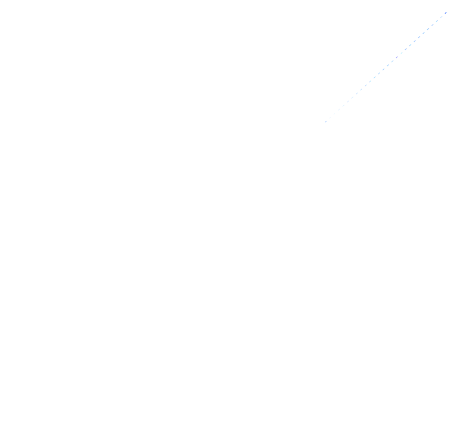
\includegraphics[width=0.9\textwidth]{2023StAndrewsAstro/Figures/fluidelement.png}
\begin{itemize}
    \item Directly modelled
    \item Kinetic, Magnetic, thermal
\end{itemize}
\end{column}
\begin{column}{0.3\textwidth}
\centering
\textbf{Ionisation/excitation energy}
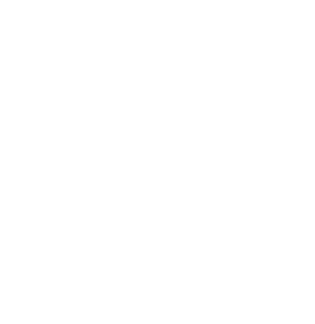
\includegraphics[width=0.8\textwidth]{2023StAndrewsAstro/Figures/ionenergy.png}
\begin{itemize}
    \item Not directly modelled but can be calculated
    \item Non-conservative 
    \item Energy remains 'in the system'.
\end{itemize}
\end{column}
\begin{column}{0.3\textwidth}
\centering
\textbf{Radiative energy}
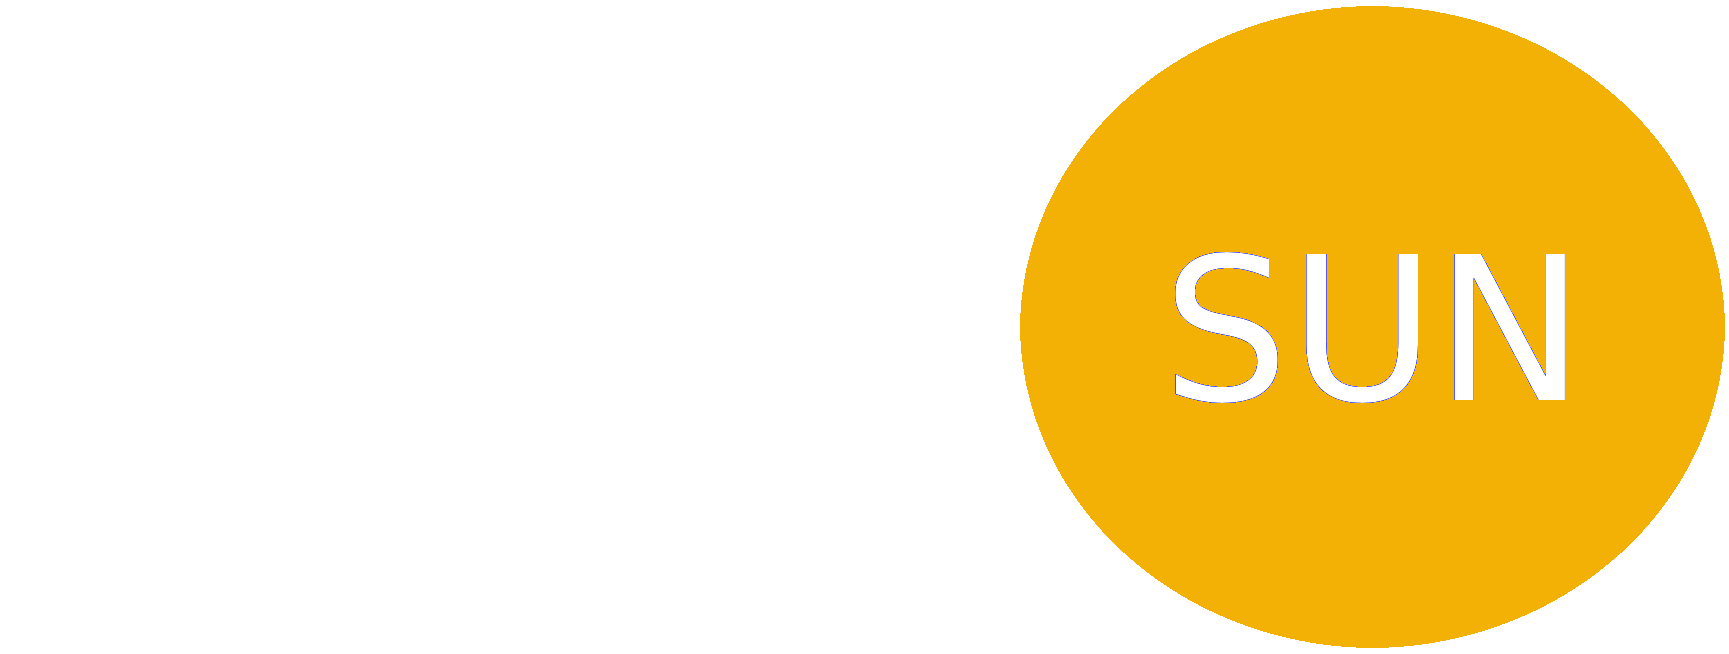
\includegraphics[width=0.8\textwidth]{2023StAndrewsAstro/Figures/radiationenergy.png}
\begin{itemize}
    \item Blackbody radiation field
    \item Not directly modelled/calculable 
    \item Allows energy to leave/enter the system
\end{itemize}
\end{column}
\end{columns}
\end{frame}

% \begin{frame}{Ionisation energy losses and recombination energy gains}
% \begin{columns}
% \begin{column}{0.4\textwidth}
% \begin{itemize}
%     \item Ionisation potential term: macroscopic energy lost during collisional ionisation. %Requires a heating term to balance.
%     \item Similar heating during collisional recombination.
%     \item Self-consistent heating/cooling mechanism.
%     \item Neutral level populations solved at each time step using excitation/de-excitation rates.
% %    \item We perform 1D two-fluid simulations of ionisation, recombination and ionisation potential terms in a slow-mode shock.
% \end{itemize}
% \end{column}
% \begin{column}{0.6\textwidth}
% \begin{gather}
%     \hat{I}_{\rm ion}= \Sigma \hat{n}_i \hat{C}_{i{\rm p}} E_i \\
%     \hat{I}_{\rm exc}= \Sigma \hat{n}_1 \hat{C}_{1u} (E_u-E_1) + \Sigma \hat{n}_2 \hat{C}_{2u} (E_u-E_2) \nonumber \\
%     \hspace{1cm} + \Sigma \hat{n}_3 \hat{C}_{3u} (E_u-E_3) + \hat{n}_4 \hat{C}_{4,5} (E_5-E_4)  \\
%     \phi_{I}=(\hat{I}_{\rm{ion}}+\hat{I}_{\rm{exc}})/\hat{\phi} 
% \end{gather}
% \begin{gather}
%     \hat{R}_{\rm rec}= \Sigma \hat{n}_{\rm p} \hat{C}_{{\rm p}i} E_i \\
%     \hat{R}_{\rm dex}= \Sigma \hat{n}_5 \hat{C}_{5l} (E_l-E_5) + \Sigma \hat{n}_4 \hat{C}_{l4} (E_l-E_4)  \nonumber \\
%     \hspace{1cm} + \Sigma \hat{n}_3 \hat{C}_{l3} (E_3-E_l) + \hat{n}_2 \hat{C}_{2,1} (E_1-E_2)  \\
%     \phi_{R}=(\hat{R}_{\rm rec}+\hat{R}_{\rm dex})/\hat{\phi} 
% \end{gather}
% \end{column}
% \end{columns}
% \end{frame}


\begin{frame}{Numerical model}
\begin{columns}
\begin{column}{0.5\textwidth}
\begin{enumerate}
\item 1D shocks in two-fluid partially-ionised plasma using (P\underline{I}P) code.
\item Investigate shock substructure.
\item Initial conditions produce switch-off slow-mode shock.
\item Initial level populations determined by reference electron number density and temperature
\item Equilibrium recombination timescale set to $10^{-5}$ of collisional timestep.
\item 512000 grid cells, 1st order HLLD solver, explicit integration of source terms.
\end{enumerate}
\end{column}
\begin{column}{0.5\textwidth}
\begin{eqnarray}
B_x &=& 0.1  \nonumber\\
B_y &=& -1.0 (x>0), 1.0 (x<0) \nonumber \\
\rho _n &=& \xi _n \rho _{tot} \nonumber \\
\rho _p &=& \xi _i \rho _{tot} = (1- \xi _n) \rho _{tot} \nonumber \\
P_n &=& \frac{\xi _n}{\xi_n + 2 \xi _i} P_{tot} =  \frac{\xi _n}{\xi_n + 2 \xi _i} \beta \frac{B_0 ^2}{2} \nonumber \\
P_p &=& \frac{2 \xi _i}{\xi_n + 2 \xi _i} P_{tot} =  \frac{2 \xi _i}{\xi_n + 2 \xi _i} \beta \frac{B_0 ^2}{2} \nonumber
\end{eqnarray}
\end{column}
\end{columns}
\end{frame}

\begin{frame}{Numerical simulation - upper chromosphere}
\begin{columns}
\begin{column}{0.8\textwidth}
\begin{figure}
    %\centering
    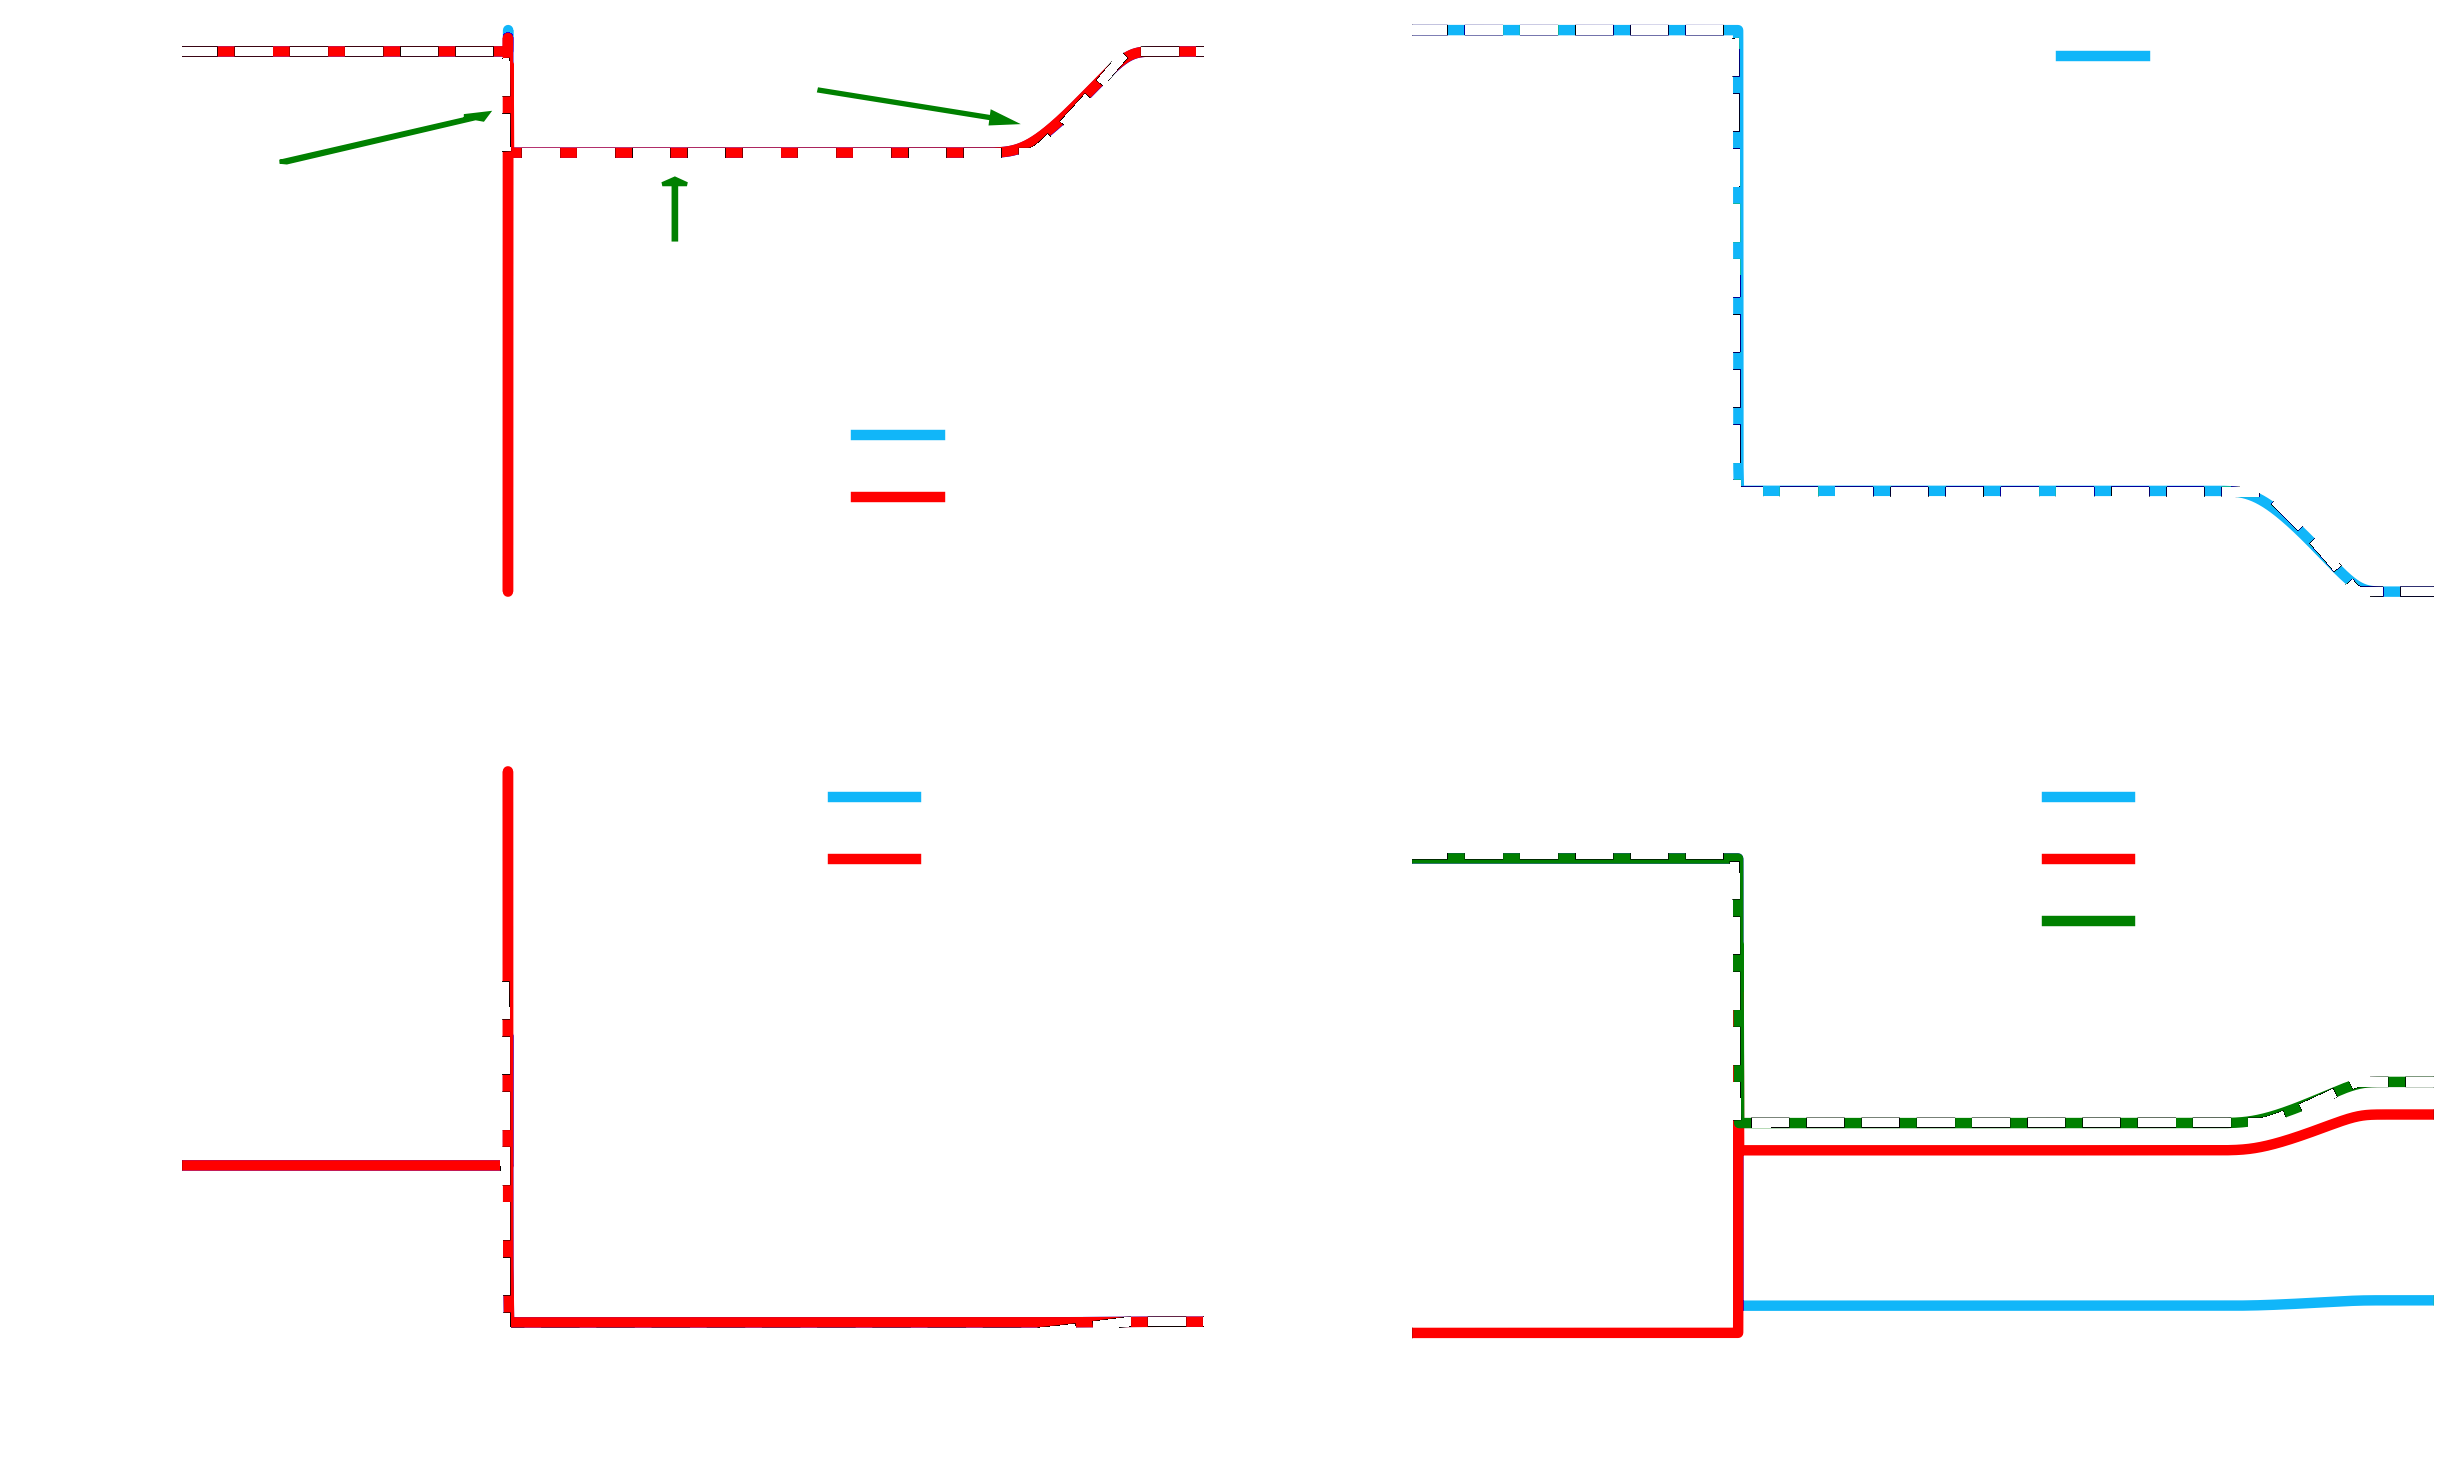
\includegraphics[width=0.95\linewidth]{2023StAndrewsAstro/Figures/context_upc_corrected.png}
    %\caption{Upper-chromosphere case showing the $v_x$ velocity (top left), $B_y$ magnetic field (top right), temperature (lower left) and density (lower right). For panel c, the reference temperature $T_0=6220$.}
    \label{fig:upperchromocontext}
\end{figure}
\end{column}
\begin{column}{0.2\textwidth}
%\begin{itemize}
    $T_0=6120$, $n_e=7.5\times 10^{16}$, $\xi_n=0.87$
%\end{itemize}
\end{column}
\end{columns}
\end{frame}

\begin{frame}{Numerical simulation - upper chromosphere}
\begin{columns}
\begin{column}{0.8\textwidth}
\begin{figure}
    %\centering
    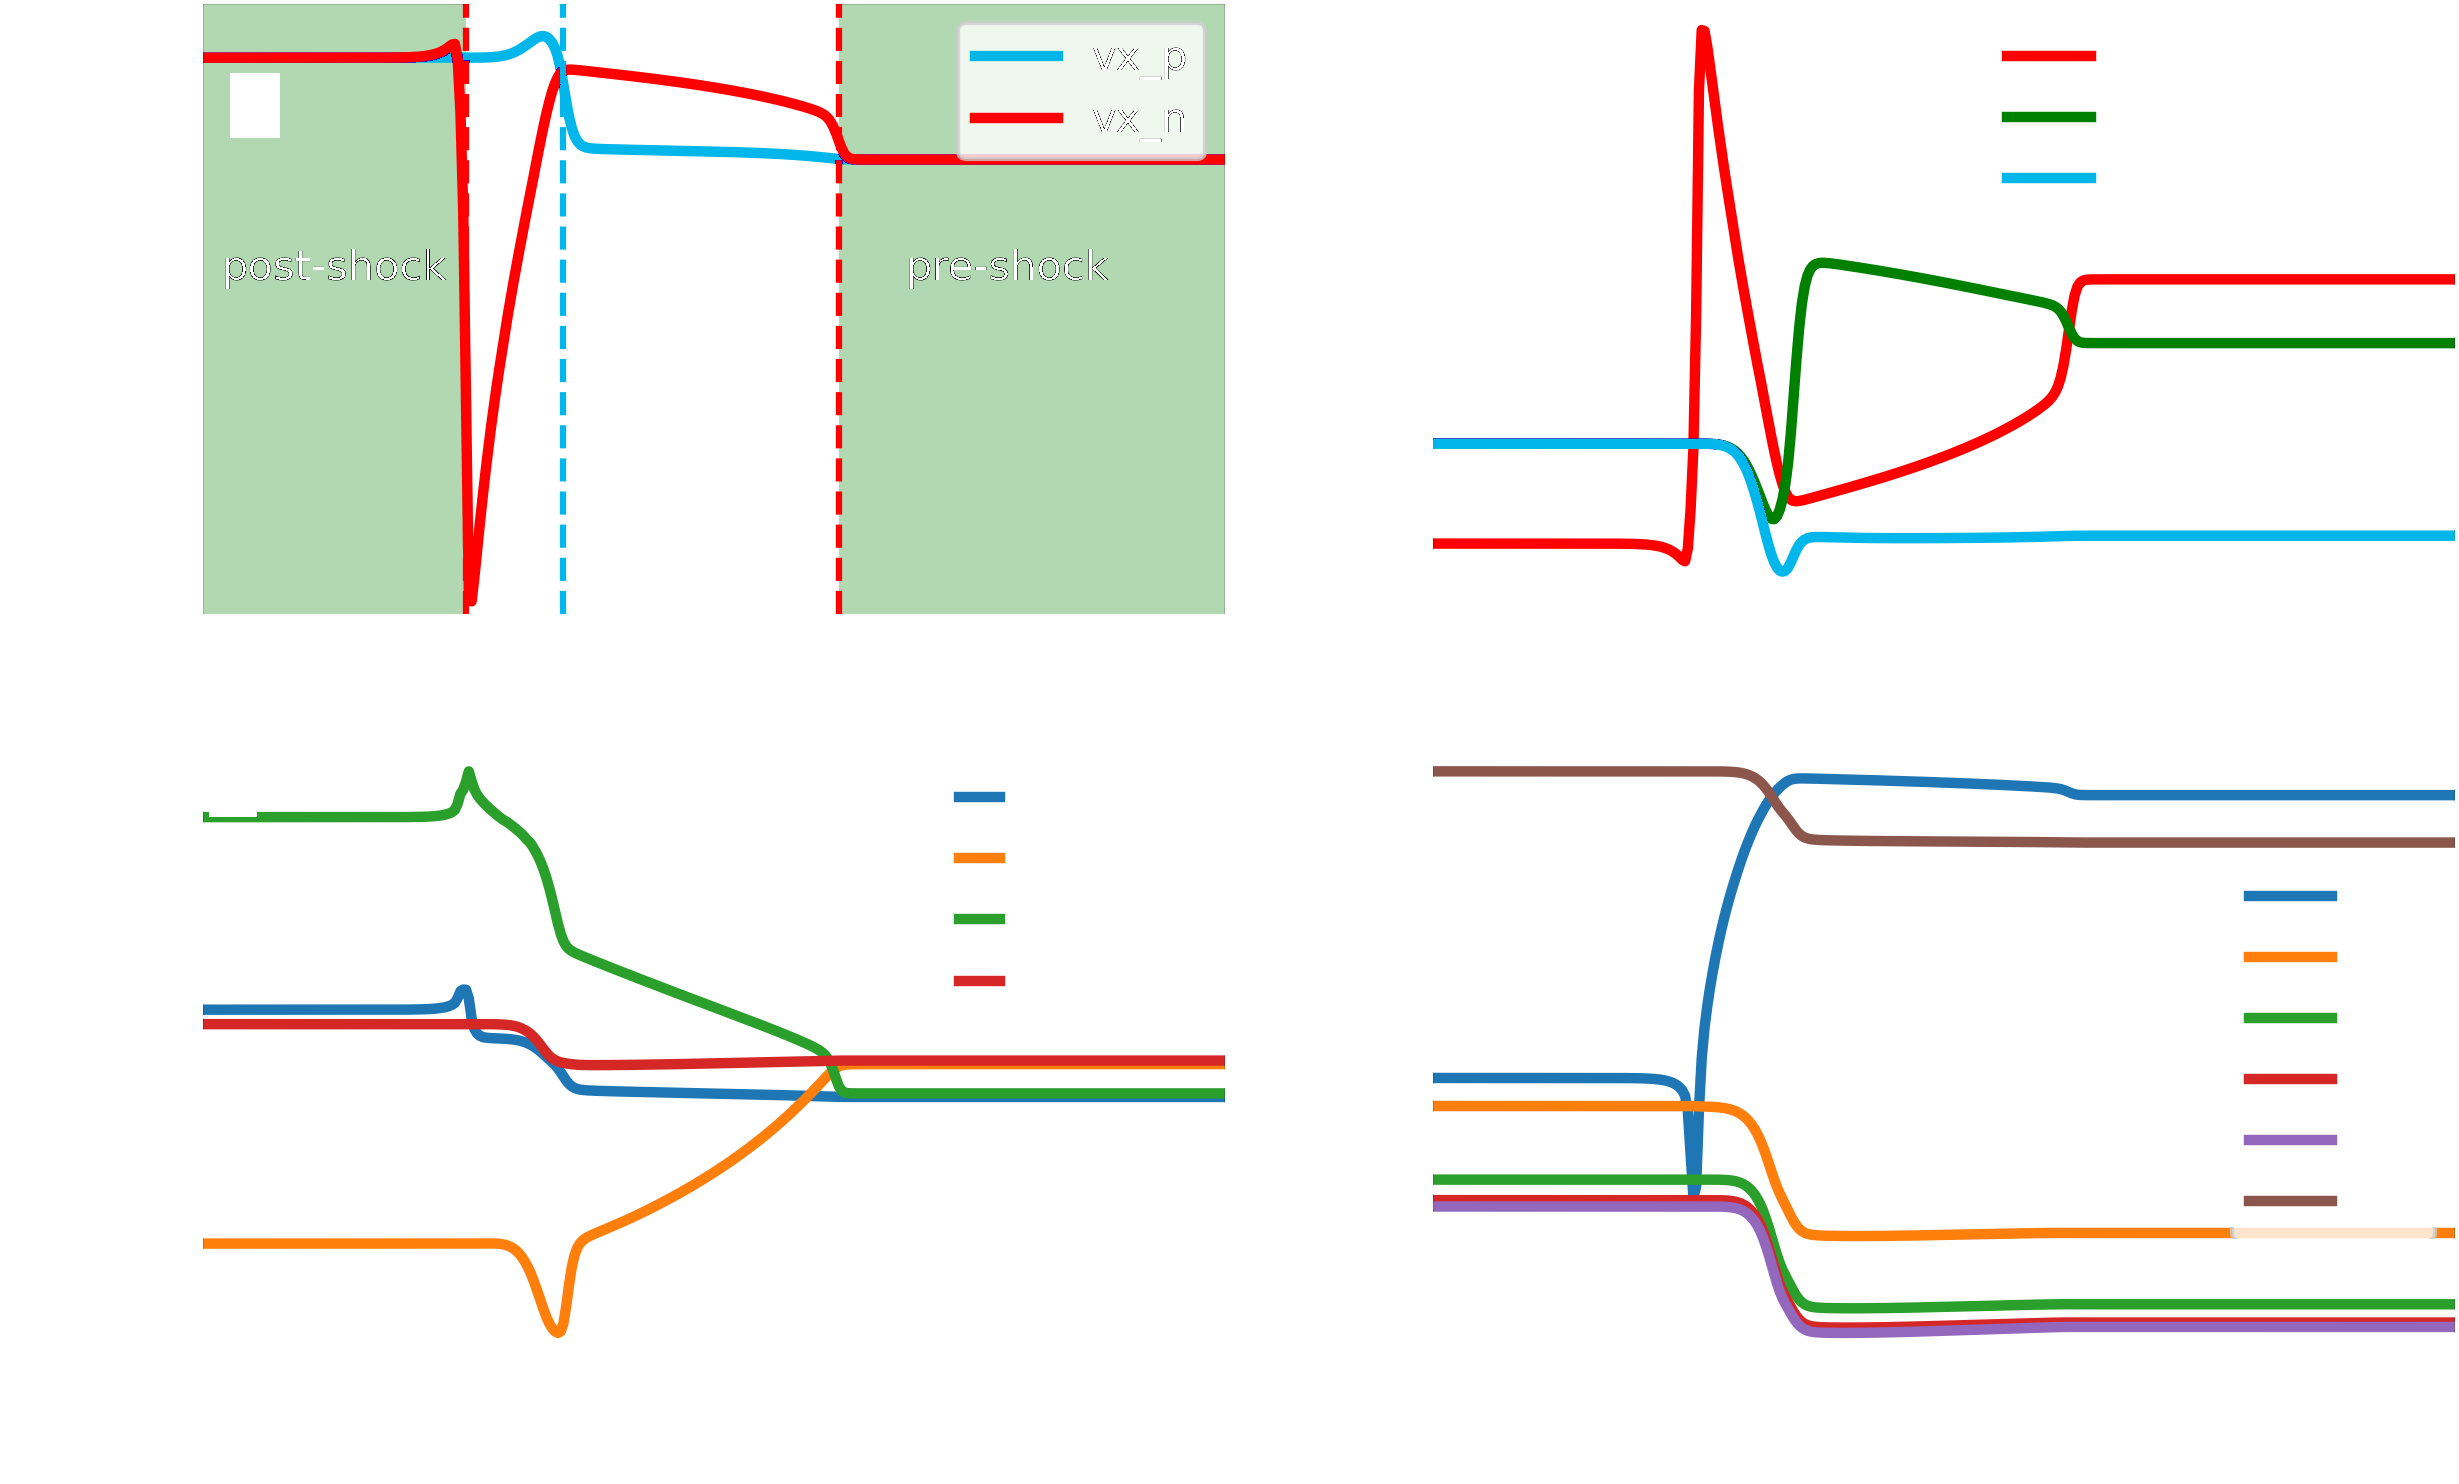
\includegraphics[width=0.95\linewidth]{2023StAndrewsAstro/Figures/shocksub2_plot_upc_corrected.png}
    %\caption{Upper-chromosphere case showing the $v_x$ velocity (top left), $B_y$ magnetic field (top right), temperature (lower left) and density (lower right). For panel c, the reference temperature $T_0=6220$.}
    \label{fig:upperchromocontext}
\end{figure}
\end{column}
\begin{column}{0.2\textwidth}
%\begin{itemize}
    $T_0=6120$, $n_e=7.5\times 10^{16}$, $\xi_n=0.87$
%\end{itemize}
\end{column}
\end{columns}
\end{frame}

\begin{frame}{Temperature thought experiment}
\begin{gather}
    T_n=\frac{\gamma P_n}{\rho_n} \mbox{\hspace{5cm}}
    T_e=\frac{\gamma P_p}{2 \rho_p} \nonumber
\end{gather}
\begin{itemize}
    \item Consider an initially neutral fluid that is spontaneously radiatively ionised
    \item Treated as energy-neutral process here, resulting in free electron with zero thermal energy (i.e., total internal energy conserved)
    \item Mass and pressure conserved but thermal energy is now shared between proton and electron
    \item Assume even split of thermal energy between proton and electron
    \item Temperature is now half the initial value
\end{itemize}
\end{frame}

\begin{frame}{Numerical simulation - mid chromosphere}
\begin{columns}
\begin{column}{0.8\textwidth}
\begin{figure}
    %\centering
    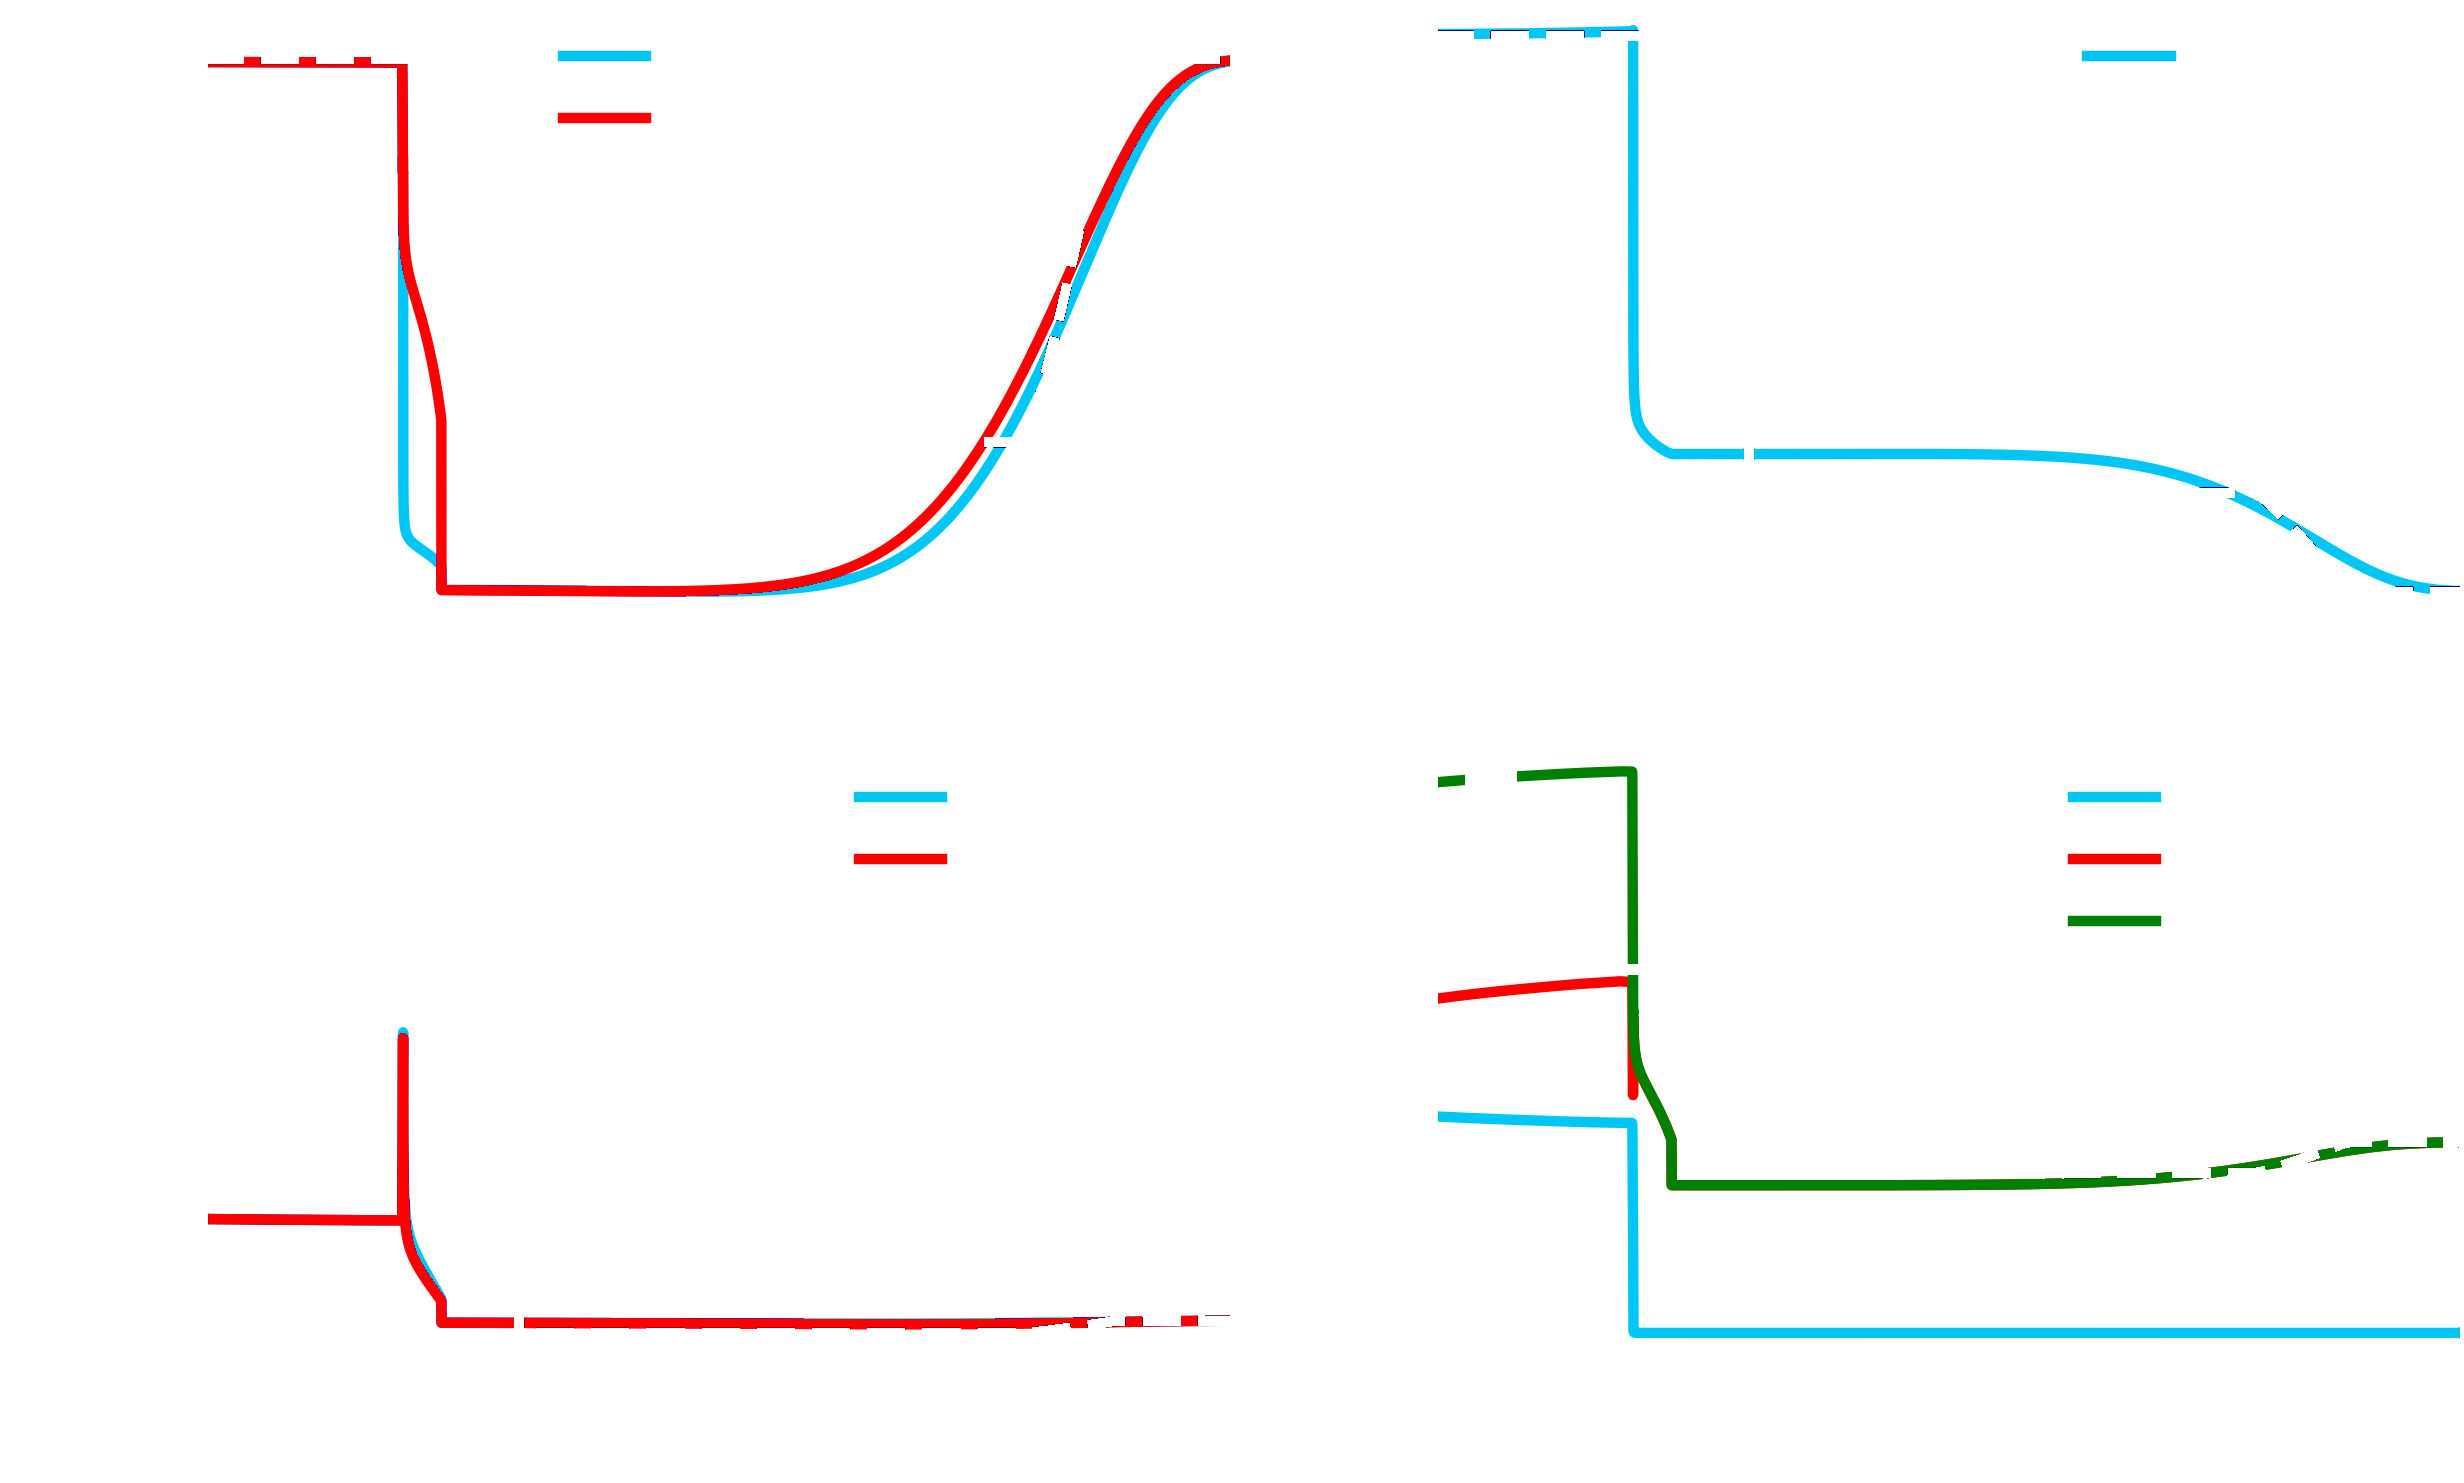
\includegraphics[width=0.95\linewidth]{2023StAndrewsAstro/Figures/context_midc_corrected.png}
    %\caption{Upper-chromosphere case showing the $v_x$ velocity (top left), $B_y$ magnetic field (top right), temperature (lower left) and density (lower right). For panel c, the reference temperature $T_0=6220$.}
    \label{fig:upperchromocontext}
\end{figure}
\end{column}
\begin{column}{0.2\textwidth}
%\begin{itemize}
    $T_0=5180$, $n_e=7.5\times 10^{16}$, $\xi_n=0.9997$
%\end{itemize}
\end{column}
\end{columns}
\end{frame}

% \begin{frame}{Numerical simulation - upper chromosphere}
% \begin{columns}
% \begin{column}{0.8\textwidth}
% \begin{figure}
%     %\centering
%     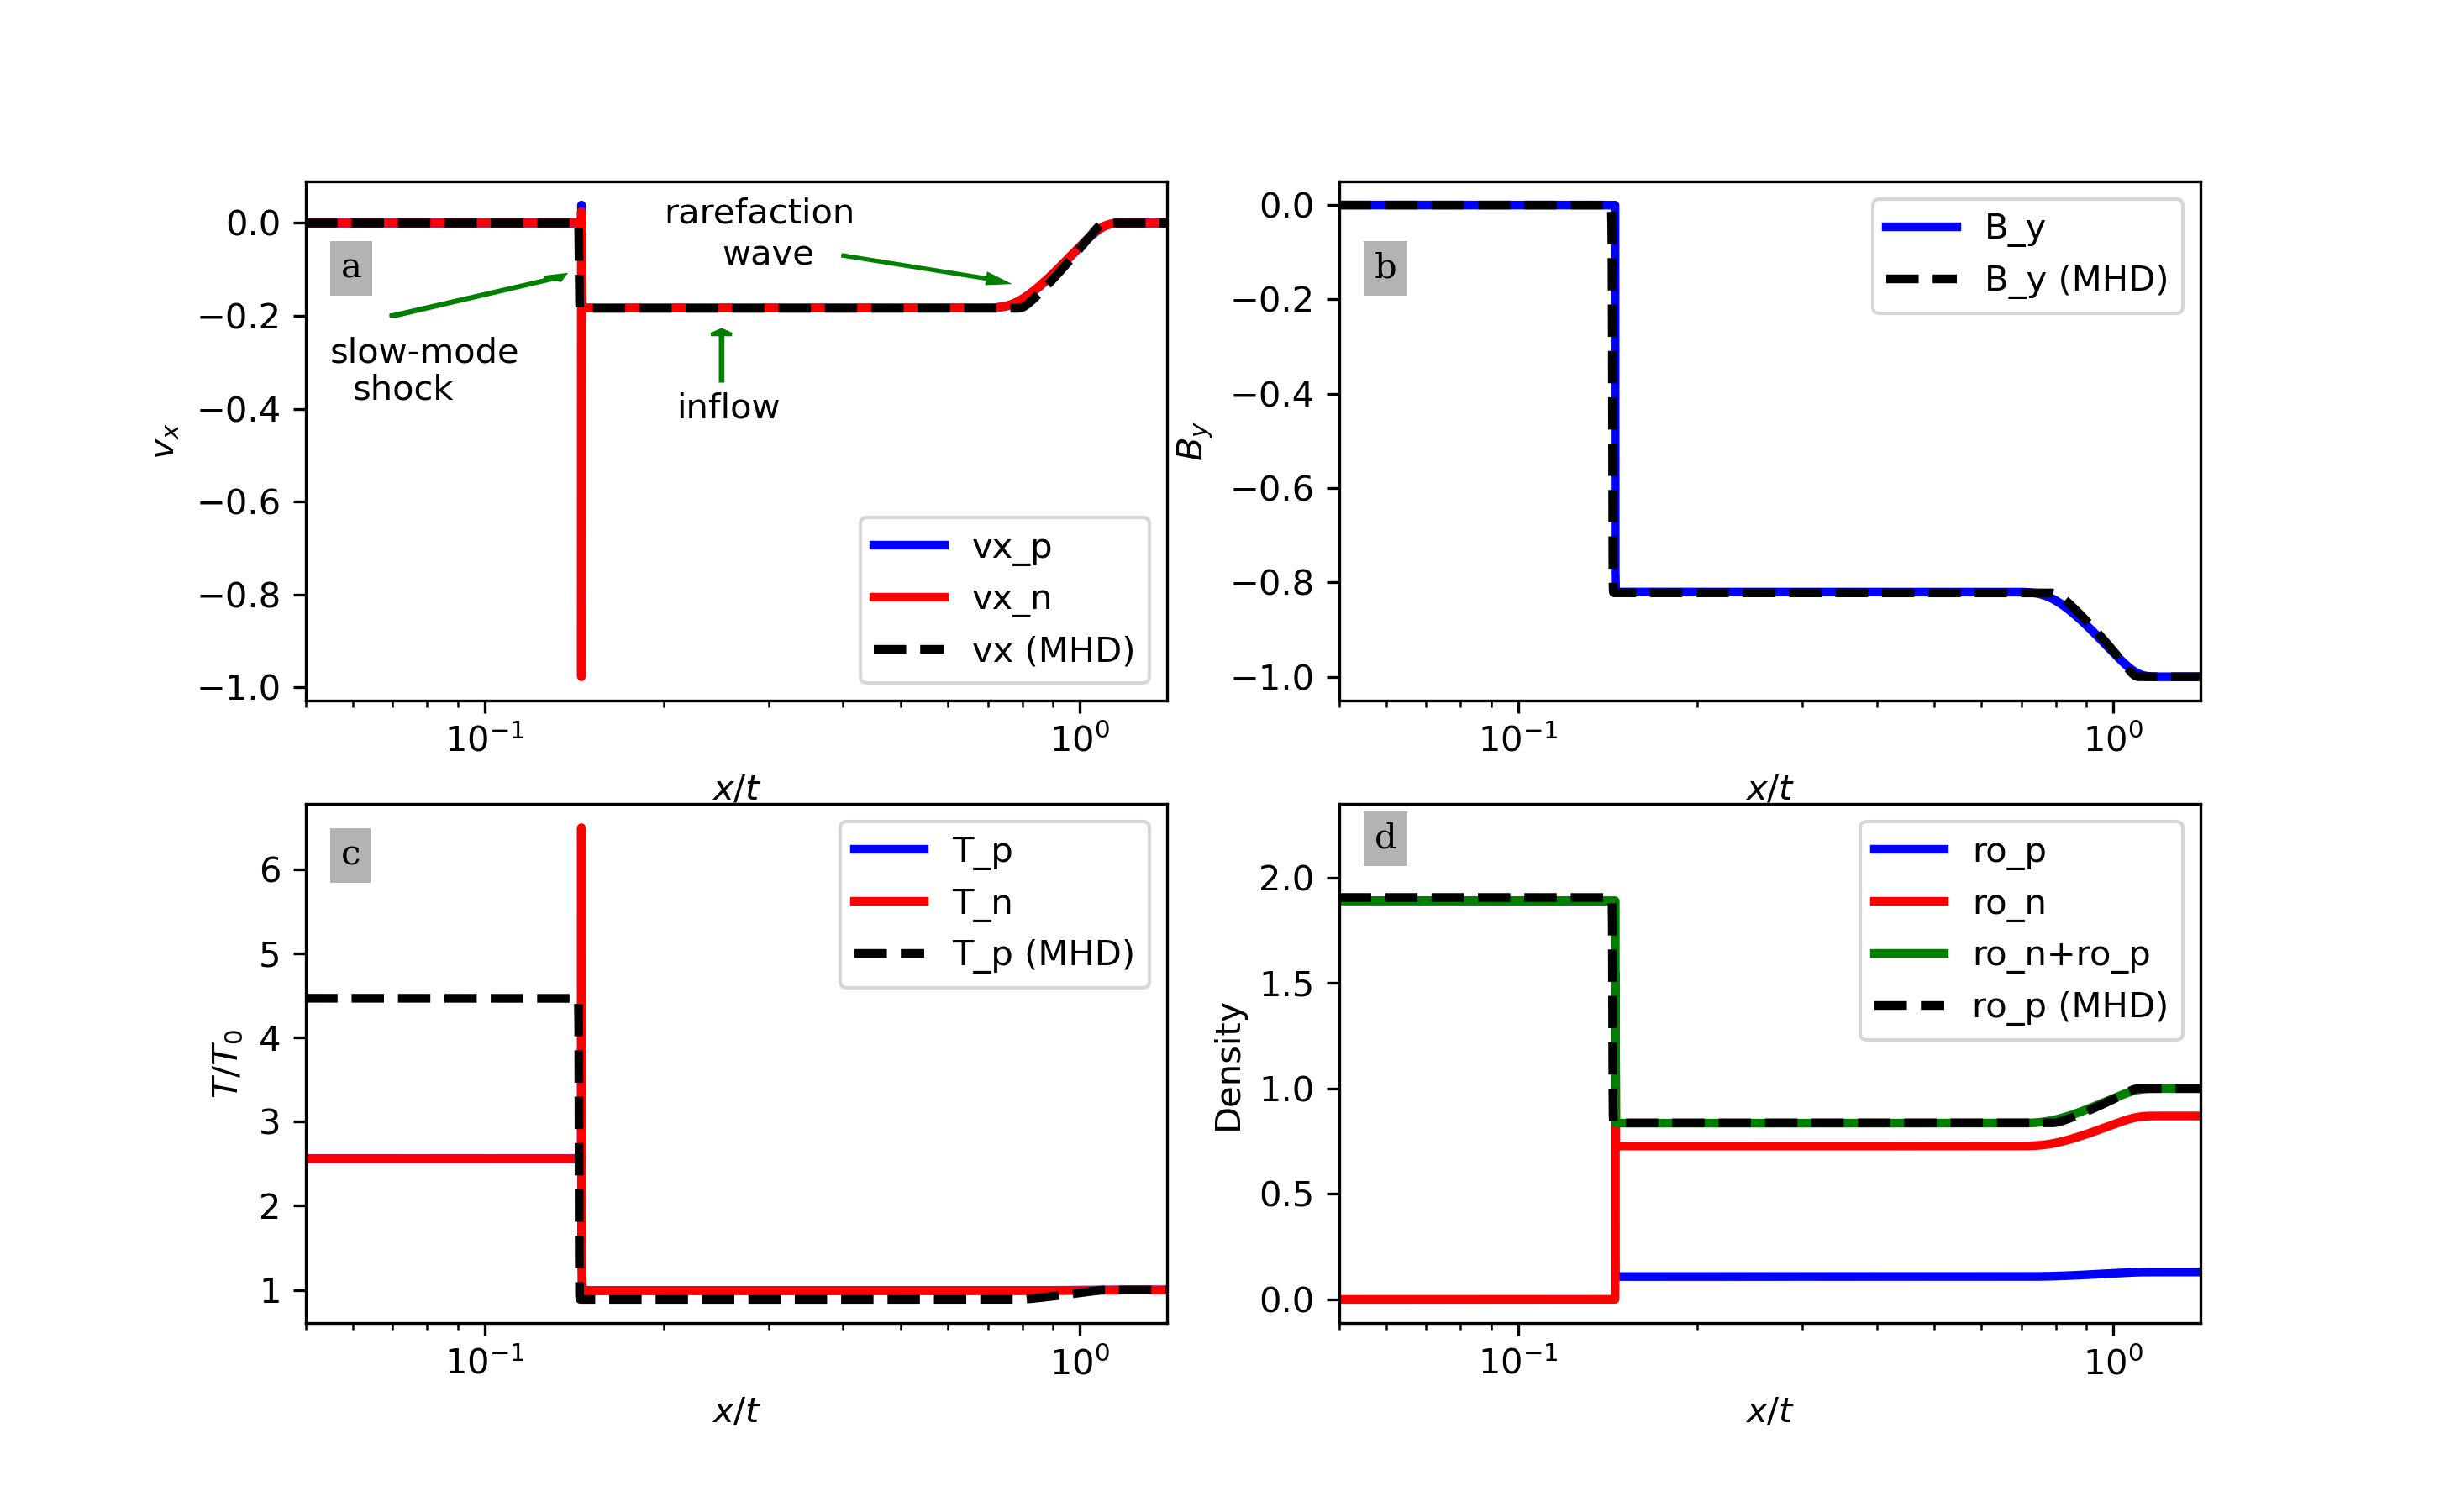
\includegraphics[width=0.95\linewidth,clip=true,trim=0.9cm 0.8cm 0.9cm 0.8cm]{2023ECRW/Figures/context_upc_corrected.png}
%     %\caption{Upper-chromosphere case showing the $v_x$ velocity (top left), $B_y$ magnetic field (top right), temperature (lower left) and density (lower right). For panel c, the reference temperature $T_0=6220$.}
%     \label{fig:upperchromocontext}
% \end{figure}
% \end{column}
% \begin{column}{0.2\textwidth}
% %\begin{itemize}
%     $T_0=6120$, $n_e=7.5\times 10^{16}$, $\xi_n=0.87$
% %\end{itemize}
% \end{column}
% \end{columns}
% \end{frame}

\begin{frame}{Shock substructure - mid chromosphere}
\begin{columns}
\begin{column}{0.8\textwidth}
\begin{figure}
    %\centering
    \includegraphics[width=0.95\linewidth]{2023StAndrewsAstro/Figures/shocksub2_plot_midc_corrected.png}
    %\caption{Upper-chromosphere case showing the $v_x$ velocity (top left), $B_y$ magnetic field (top right), temperature (lower left) and density (lower right). For panel c, the reference temperature $T_0=6220$.}
    \label{fig:upperchromocontext}
\end{figure}
\end{column}
\begin{column}{0.2\textwidth}
%\begin{itemize}
    $T_0=5180$, $n_e=7.5\times 10^{16}$, $\xi_n=0.9997$
%\end{itemize}
\end{column}
\end{columns}
\end{frame}

%%%%%%%%%%%%%%%%%%%%%%%%%%%%%%%%%%%%%%%%%%%%%%%%%%%%%%%%%%%%%%%%%%%%%%%%%%%%%%%%

\begin{frame}{Cooling through the shock}
\begin{columns}
\begin{column}{0.5\textwidth}
\begin{figure}
    \centering
    \includegraphics[width=0.95\linewidth]{2023StAndrewsAstro/Figures/tcompcor_plot.png} \\
    %\includegraphics[width=0.95\linewidth,clip=true,trim=0.4cm 0.3cm 0.1cm 1.8cm]{2023ECRW/Figures/tcompcor_ion_plot.png}
\end{figure}
\end{column}
\begin{column}{0.42\textwidth}
%\includegraphics[width=0.95\linewidth,clip=true,trim=0.2cm 0.3cm 0.0cm 1.6cm]{2023ECRW/Figures/tcomploss_plot.png}
\begin{itemize}
    %\item Constant reference electron number density
    \item Temperature increase much less than predicted by MHD
    \item Density increase much greater than MHD
    \item Rankine-Hugoniot jump conditions may not apply to lower atmosphere shocks
    %\item Observational consequences?
\end{itemize}
\end{column}
\end{columns}
\end{frame}

%%%%%%%%%%%%%%%%%%%%%%%%%%%%%%%%%%%%%%%%%%%%%%%%%%%%%%%%%%%%%%%%%%%%%%%%%
\begin{frame}{Conclusion}
\begin{itemize}
    \item Partially-ionised shocks are far from understood. 
    \item When we include the relevant physics, shocks heat much less than expected! Cooling solutions possible.
    \item Explain solar observations - DKIST (French+2023)
    \item Connection to astrophysics - partially-ionised shocks non-unique to solar atmosphere
    \item Approach here is for arbitrary hydrogen plasma.
\end{itemize}
\end{frame}

%%%%%%%%%%%%%%%%%%%%%%%%%%%%%%%%%%%%%%%%%%%%%%%%%%%%%%%%%%%%%%%%%%%%%%%%%
% \begin{frame}{Connections to astrophysics}
% \begin{itemize}
%     \item Partially-ionised shocks are not unique to the solar atmosphere.
%     \item Modelling approach is for an arbitrary hydrogen plasma.
% \end{itemize}
% \end{frame}


%%%%%%%%%%%%%%%%%%%%%%%%%%%%%%%%%%%%%%%%%%%%%%%%%%%%%%%%%%%%%%%%%%%%%%%%%
% \begin{frame}{Future research}
% \begin{itemize}
%     \item Reconnection studies- ongoing
%     \item ERF proposal - adapt for Leverhulme, etc.
%     \item Explain observations
%     \item Fits within the MHD group at Dundee MAKE STRONGER
% \end{itemize}
% \end{frame}

%%%%%%%%%%%%%%%%%%%%%%%%%%%%%%%%%%%%%%%%%%%%%%%%%%%%%%%%%%%%%%%%%%%%%%%%%
% \begin{frame}{How this fits into Dundee's existing group}

% \end{frame}

\end{document}
